\begin{document}

\author{Prof.~G.~Averkov\\{\small Institut für Mathematik, Fakultät 1}\\{\small Fachgebiet Algorithmische Mathematik}\\{\small Brandenburgische Technische Universität Cottbus}}
\title{\Huge{\sc{Mathematik IT-3}}\\ \Large{\sc{Mathematik für Informatik-Studiengänge}: Analysis}}
\date{\today}

%\frontmatter
\mainmatter
%\maketitle
\thispagestyle{empty}
\begin{center}
	\Huge{\sc{Mathematik IT-1}}\\ \Large{\sc{Diskrete Mathematik für Informatik-Studiengänge}}
	\\ \normalsize{\today}
	\\ {\ }
	\\ \large{Prof.~G.~Averkov} 
	\\{\small Institut für Mathematik, Fakultät 1}\\{\small Fachgebiet Algorithmische Mathematik}\\{\small Brandenburgische Technische Universität Cottbus-Senftenberg}
\end{center} 

\tableofcontents

\chapter*{Organisatorisches} 

\begin{bem}[Vorlesung] {\ } 
	\begin{enuma} 
		\item In Präsenz, digitale Mitschrift im Moodle, bei Bedarf Aufzeichnungen 
		\item In der Vorlesung geht es um die Theorie und Ihre Rolle bei der Lösung von Aufgaben. 
		\item  Theorie ist ein Werkzeug zur Lösung von Problemen und Aufgaben.
	\end{enuma}
\end{bem} 


\begin{bem}[Übung]{\ } 
	\begin{enuma} 
		\item Zwei Übungstermine pro Woche.
		\item Eine synchron und eine asynchron über BigBlueButton
		\item Die Teilnehmer werden \underline{nicht} in zwei Übungsgruppen eingeteilt. Jede Woche kann eine der beiden Übungen frei gewählt werden. 
		\item Aufgabenblatt Nummer $x$ (mit $x \ge 1$) wird in der Vorlesungswoche $x+1$ diskutiert und zum Ende der Woche $x$ abgegeben. 
		\item Abgabe der Blätter digital über Moodle. 
		\item Blatt Nummer $0$ wird in der ersten Woche diskutiert und wird nicht abgegeben. 
	\end{enuma} 
\end{bem} 


\begin{bem}[Prüfung]{ \ } 
	\begin{enuma} 
		\item Zulassung zur Klausur bei mind. $50\%$ aller Punkte für die Aufgabenblätter 
		\item Bei mind. $75\%$ aller Punkte für die Aufgabenblätter gibt es einen $10\%$ Bonus in der Klausur
		\item Keine Rechengeräte in der Klausur zugelassen
	\end{enuma} 
\end{bem} 

\chapter*{Einleitung}

\section{Wissenschaftliche Prinzipien}

\begin{bem}\ 
\begin{itemize}
	\item Möglichst wenig Annahmen, insb. keine überflüssigen Annahmen. 
	\item Überprüfung von Behauptungen : Beobachtungen, Experimente, Argumente. 
	\begin{itemize}
		\item Schwerpunkt bei Mathe: Argumente 
		\item Experimente bei Mathe meistens billig: Beispiele, Skizzen 
	\end{itemize} 
	\item Die Autorität zählt nicht (``Aber mein Lehrer hat gesagt, dass das so richtig ist''), es zählen validierte Behauptungen. 
	\item Begriffe/Bezeichnungen werden möglichst eindeutig festgelegt (bei Mathe - extrem eindeutig),  so dass man möglichst keinen Spielraum für eine Interpretation haben soll. (``War das die wahre Liebe?'' - kann man die Liebe eindeutig definieren? Wenn nicht, dann kann man so eine Art Frage endlos diskutieren, ohne Ergebnis. ). ``Die Erde ist rund'' - was heißt genau ``die Erde''? Was heißt genau ``rund''? Begriffsklärung sehr wichtig. 
	\item Naturwissenschaften (Reale Welt und Modelle dazu) und  Strukturwissenschaften (Modelle). 
	\item Grundlagenwissenschaften: wenn man oft genug ``Warum?'' fragt, kommt man zu grundlegenden Fragen, deren Antworten einen bleibenden Wert und -- auf Dauer -- breite Anwendungsmöglichkeiten haben. Wichtige Frage: Warum? Warum gibt uns die $pq$-Formel das richtige Ergebnis? Die Antwort ist für die Mathe-Gemeinschaft interessanter als die Formel selbst. Das Interessante in der Mathematik ist genau das, was man in den Formeltafeln nicht findet. 
\end{itemize} 
\end{bem}


\section{Mathematische Prinzipien} 

\begin{bem}\ 
\begin{itemize}
		\item Für eine mathematische Theorie legt man Grundbegriffe und Grundbezeichnungen (eindeutig) fest. 
		\item Auf der Basis der bereits vorhandenen Begriffen und Bezeichnungen führt man immer neue Begriffe und Bezeichnungen (eindeutig) ein. 
		\item Mit Hilfe von vorhandenen Begriffen und Bezeichnungen werden Aussagen formuliert, die dann durch Argumentation bestätigt ($=$ bewiesen) oder widerlegt werden. 
		\item Wahre mathematische Beweise sind widerspruchsfrei und vollständig. 
		\item In der Theorie interessiert man sich vor allem für noch offene Aussagen, die aktuell weder bestätigt noch widerlegt worden sind. 
		\item Mathematik $\ne$ Rechnen. Rechnen, ohne dass man versteht, was die Rechenschritte bedeuten, ist keine mathematische Tätigkeit. Wichtig ist der Sinn hinter den Rechenschritten. Erkennt man beim Rechnen den Sinn nicht, dann ist man ein menschlicher Computer (echte Computer machen weniger Fehler und sind etwas schneller beim Rechnen :)) 
\end{itemize} 
\end{bem} 

\chapter{Mathematische Grundlagen}

\section{Aussagen und logische Verknüpfungen}


\begin{defn}
Eine Aussage ist ein Satz (eine Folge von Zeichen mit mathematischer Bedeutung), die einen eindeutigen Wahrheitswert (entweder falsch oder wahr) hat. Den Wahrheitswert kodiert man oft mit Zahlen $0$ (falsch) und $1$ (wahr). 
\end{defn} 


\begin{bsp}\ 
\begin{itemize}
	\item $ 2 < 1 $ (falsch)
	\item $ 2 = 1 $ (falsch)
	\item $ 2 > 1 $ (wahr)
	\item $2$ ist eine Primzahl (wahre Aussage, Primzahl definiert). 
	\item $2$ ist eine schöne Zahl (keine Aussage, es sei denn, die Eingeschaft einer Zahl schön zu sein, wurde definiert). 
	\item Es gibt unendlich viele Primzahlen $n$, für welche $n+2$ ebenfalls eine Primzahl ist. (eine Aussage, Wahrheitswert ist noch nicht geklärt). 
	\item Die Gleichung $x^2+1 =0$ hat keine Lösungen. (an sich keine Aussage, es sei denn, ein Kontext war vorher gegeben, in dem die Rolle von $x$ geklärt wuirde.)
	\item Die Gleichung $x^2+1=0$ hat keine reellwertigen Lösungen (wahre Aussage). 
\end{itemize}
\end{bsp} 

\begin{defn}
Seien $ A $ und $ B $ Aussagen. Dann definiert man anhand von $ A $ und $ B $ die folgenden Aussagen:
\begin{itemize}
	\item $ A \wedge B $ Konjunktion (\glqq und\grqq) ist genau dann wahr, wenn $A$ und $B$ beide wahr sind. 
	\item $ A \vee B $ Disjunktion (\glqq oder\grqq) ist genau dann falsch, wenn $A$ und $B$ beide falsch sind. 
	\item $ A \Rightarrow B $ Implikation ist genau dann falsch, wenn $A$ wahr und $B$ falsch ist. 
	\item $ A \Leftrightarrow B $ Äquivalenz ist genau dann wahr, wenn die Wahrheitswerte von $A$ und $B$ gleich sind. 
	\item $ A \:\dot{\vee}\: B $ ausschließende Disjunktion ist genau dann wahr, wenn die Wahrheitswerte von $A$ und $B$ verschieden sind. 
	\item $ \neg A $ (wir auch als $ \bar{A} $ bezeichnet), Negation (Verneinung) ist genau dann wahr, wenn $A$ falsch ist. 
\end{itemize}
\end{defn}


\begin{bsp}\
	\begin{itemize}
		\item Seien $ x,y \in \R$. Dann gilt die Implikation: $x = y \Rightarrow x^2 = y^2 $ (wahr)
		\item Seien $x,y \in \R$. Dann gilt die Implikation $ x,y \in \R, x^2 = y^2 \Rightarrow x = y $ (falsch für $x=1$ und $y=-1$)	
	\end{itemize}
\end{bsp}

\begin{bem}
	Alternativbezeichnungen für $\Rightarrow$ und $\Leftrightarrow$ sind $\rightarrow$ bzw. $\leftrightarrow$. 
\end{bem} 

\begin{bem}
	Wenn man in Mathe-Argumenten eine Folge von Implikationen benutzt, so schreibt man auch oft kurz so etwas wie $A \Rightarrow B \Rightarrow C$. Damit meint man  $(A \Rightarrow B) \wedge (B \Rightarrow C)$, d.h., aus $A$ folgt $B$ und aus $B$ folgt $C$. Das Gleiche auch für $\Leftrightarrow$. 
\end{bem} 


\begin{bem}
	Die Aussagenlogik ist die Studie der logischen Vernknüpfungen von Aussagen. Dabei spielt die Natur in den Formeln verwendeten Aussagen, die man mit Symbolen bezeichnet, etwa $a,b, c, d, \ldots$, an sich keine Rolle. Alles, was zählt, ist der Wahrheitswert. Daher kann man auch $a,b,c,d \ldots$ als Variablen aus $\{0,1\}$ auffassen, ohne dass sich an der Studie was ändert. Mehr über die Aussagenlogik erfahren wir später in diesem Kurs. 
\end{bem} 

\clearpage
\section{Mengen und Mengenoperationen}


\begin{defn}[Intuitive ``Definition'' einer Menge] 
	Eine Menge $X$ ist durch die Eindeutige Angabe definiert, welche Objekte Elemente der Menge sind. Man schreibt in diesem Fall $x \in X$ dafür, dass das Objekt $x$ Element der Menge $X$ ist, und $x \not\in X$ dafür, dass $x$ kein Element der Menge $X$. 
	
	Mit anderen Worten: für die Angabe einer Menge $X$ soll für jedes Objekt $x$ geklärt sein, ob für dieses Objekt $x \in X$ oder $x\not \in X$ gilt. 
\end{defn} 

\begin{bem}[Zur korrekten Definition einer Menge]
	Unsere Definition der Menge ist etwas intuitiv und  somit streng genommen keine echte Definition); sie reicht aber vorerst für unsere Zwecke völlig aus. Die genaue Definition einer Menge ist durch das Axiomensystem von Zermelo-Fraenkel gegeben. Dieses System legt Folgendes fest: 
	\begin{itemize}
		\item die Existenz der leeren Mengen, 
		\item die Bedingung für die Gleichheit von zwei Mengen
		\item die Möglichkeit Mengenfamilien zu vereinigen, 
		\item die Existenz einer sogenannten Potenzmenge für eine beliebige Menge
		\item Fundierungsaxiom (ist etwas technisch)
		\item die Möglichkeit Mengen, durch eine Bedingung zu definieren. 
		\item Ersetzungsaxiom (ist etwas technisch)
	\end{itemize} 
	Zu den obigen Axiomen nimmt man noch zusätzlich das sogenannte Auswahlaxiom dazu. Das Axiomensystem, das auf diese Weise entsteht, wird als ZFC (Zermelo-Fraankel axioms plus Axom of Choice) abgekürzt. 
\end{bem} 


\begin{bsp}[Definition einer Menge durch endliche/unendliche Auflistung] 
Eine Weise, Mengen zu definieren, ist durch die Auflistung ihrer Elemente. Dabei stehen die geschweiften Klammern für Mengen, die drei Punkte bedeuten \glqq usw\grqq.
\begin{itemize}
	\item $ \{1,2,5,7\} $ - Menge aus den vier Elementen $1,2,5$ und $7$. 
	\item $ \{1\} $ - Menge aus einem einzigen Element $1$. 
	\item $ \{1,\{2,5\},\{6\}\} $ - Menge aus drei Elementen, von denen zwei Elementen selber Mengen sind. 
	\item $ \{1,2,3,\ldots\} $ - Menge der aller positiven ganzen Zahlen. 
\end{itemize}
\end{bsp}

\begin{defn}
Seien $ A $ und $ B $ Mengen. Dann heißt $ A $ eine \textbf{Teilmenge} von $ B $, wenn jedes Element von $ A $ auch Element von $ B $ ist;  wir verwenden in diesem Fall die Bezeichnung $A \subseteq B$ und nennen die Relation $\subseteq$ \textbf{Inklusion}. 

Wenn $A$ Teilmenge von $B$ aber $B$ keine Teilmengen von $A$ ist, so sagt man, dass $A$ eine \textbf{echte Teilmenge} von $B$ ist; wir verwenden in diesem Fall die Bezeichnung $A \varsubsetneq B$ und nennen die Relation $\varsubsetneq$ eine \textbf{echte} bzw. \textbf{strikte Inklusion}. 
\end{defn}

\begin{bem}
In einigen mathematischen Quellen bezeichnet man die Inklusion als $ \subset $ und nicht als $ \subseteq $. Es ist schwer zu sagen, welche Bezeichnung in der Mehrheit der Quellen benutzt wird. Es gibt aber auch Quellen, in denen $ \subset $ die strikte Inklusion bezeichnet. Durch die Nutzung $\subseteq$ vermeiden wir potenzielle Ambiguitäten. 
\end{bem} 

\begin{defn}
	 Mengen $ A $ und $ B $ heißen \textbf{gleich}, wenn $ A \subseteq B $ und $ B \subseteq A $ gilt. 
\end{defn} 


\begin{bem}[Definition einer Menge durch eine Bedingung]
Eine sehr verbreite Weise, Mengen zu definieren, ist durch Bedingungen, nach dem Format 
\[
 \setcond{ \text{AUSDRUCK} }{\text{BEDINGUNG}}. 
\] Der Doppelpunkt bedeutet so viel wie \glqq sodass\grqq oder \glqq mit der Bedingung\grqq. In manchen Quellen wird ein Strich an der Stelle des Doppelpunktes benutzt. 
\end{bem} 

\begin{bem} In der Programmiersprache Python hat man den Datentyp Menge sowie syntaktische Strukturen zur Konstruktion von Mengen und Listen, die analog zu mathematischen Bezeichnungen sind: 
\begin{center}
	\small 
	\begin{tabular}{l|l}
		Mathematik & Python 
\\ \hline	$\{1,2,5,7\}$ 
& \begin{lstlisting}[language=Python,backgroundcolor=\color{white}]
set([1,2,5,7])
\end{lstlisting} 
\\ $\setcond{i \in \Z}{0 \le i < 6}$ & 
\begin{lstlisting}[language=Python,backgroundcolor=\color{white}]
set(range(6))
\end{lstlisting} 
\\ $\setcond{i ^2}{i \in \Z, \ 0 \le i < 6}$
&  
\begin{lstlisting}[language=Python,backgroundcolor=\color{white}]
set([i**2 for i in range(6)])
\end{lstlisting} 
\\ $\setcond{i^2}{i \in \Z, \ 0 \le i < 6, \ i \ \text{ungerade}}$
& 
\begin{lstlisting}[language=Python,backgroundcolor=\color{white}]
set([i**2 for i in range(6) if i%2==1])
\end{lstlisting} 
\end{tabular}
\end{center}  
\end{bem} 

\begin{aufg}\ 
\begin{itemize}
\item Bestimmen Sie, welche der Zahlen $1,\ldots, 100$ Elemente der Menge 
\[
	 \{ k^2 : k \in \N, k \: \text{ungerade} \} 
\]
sind. 
\item Wie viele Elemente hat die Menge $\setcond{x \in \R}{x^2- 5 x + 6} $? Welche Elemente sind es genau? 
\end{itemize}
\end{aufg}

\begin{defn}
Die \textbf{leere Menge} ist die Menge, die keine Elemente enthält; sie wird als $ \emptyset $ bezeichnet. 
\end{defn} 

\begin{defn}[Potenzmenge]
Sei $ X $ eine Menge. Dann ist die \textbf{Potenzmenge} von $ X $ die Menge aller Teilmengen von $ X $; für diese Menge benutzen wir die Bezeichnung $ 2^X $. Nach unserer Definition ist $2^X$ als  
\[
	 2^X := \{ A : A \subseteq X \} .
\]
gegeben. 
\end{defn} 

\begin{bem} Hier und im folgenden verwenden wir die Gleichung $:=$ mit Doppelpunkt, wenn es um neue Bezeichnungen geht, die festgelegt werden. Format: 
	\[
		\text{NEUE BEZEICHNUNG} := \text{BEDEUTUNG DER BEZEICHNUNG}
	\]
	Die Nutzung vom Doppelpunkt in diesem Fall ist kein Muss; man kann auch durch den Begleittext verdeutlichen, dass man eine neue Bezeichnung einführt. 
\end{bem} 

\begin{aufg}
	Wenn $X$ genau $n \in \N$ Elemente hat, wie viele Elemente hat $2^X$? Was wäre Ihre Begründung dazu? 
\end{aufg} 

\begin{bem}
	Eine weitere Bezeichnung fúr die Potenzmengen, die man in der Literatur benutzt, ist $\mathcal{P}(X)$. Ich persönlich finde $2^X$ einleuchtender (zumindest im Kontext der Kombinatorik, die im folgenden Kapitel diskutiert wird). 
\end{bem} 


\begin{bem}
	Zahlenbereiche, die Sie evtl. aus der Schule schon kennen:
\begin{itemize}
\item[$ \N $] $ := \{ 1,2,3,\ldots \} $ die Menge der natürlichen Zahlen. Uns fehlt dort die Null, daher... 
\item[$ \N_0 $] $ := \{ 0,1,2,\ldots \} $. Hier können wir nicht beliebig subtrahieren, daher... 
\item[$ \Z $] $ := \{ 0,1,-1,2,-2,\ldots \} $ die Menge der ganzen Zahlen. Hier können wir nicht beliebig dividieren, daher...
\item[$ \Q $] $ := \{ \frac{p}{q} : p \in \Z, q \in \N \} $ die Menge der rationalen Zahlen. In dieser Menge gibt es ``Löcher'' , die man merkt, wenn man Geometrie oder Analysis macht. Gemeint ist das Folgende: betrachtet man unendliche viele rationale Zahlen $a_1 \le a_2 \le a_3 \le \cdots $ und $ \cdots \le b_3 \le b_2 \le b_1$ mit $a_n \le b_n$ für jedes $n \in \N$, so gibt es nicht immer eine \underline{rationale} Zahl $x$ die $a_n \le x \le b_n$ für alle $n \in \N$ erfüllt. Informell: zwischen zwei Schranken $a_n$ und $b_n$, die sich mit jeder ``Iteration'' $n \in \N$ immer verbessert, wird nicht immer eine rationale Zahl eingefangen. In diesem Fall kann man von einem ``Loch'' spricht. Durch reelle Zahlen werden solche Löcher gestopft. 
\item[$ \R $] die Menge der reellen Zahlen. Format einer reellen Zahl: Vorzeichen $\pm$ endlich viele Stellen vor dem Komma, unendlich viele Nachkommastellen. Wir benutzen gerne die Computer-Formatierung mit Punkt an der Stelle von Komma (weil man in Mathe die Kommas gerne für viele andere Zwecke benutzt). Beispiele: 
\begin{itemize}
	\item[] $0{.}00000\cdots$ ist die $0$, 
	\item[] $1{.}00000 \cdots$ ist die $1$ 
	\item[] $-0{.}99999 \cdots$ ist das selbe wie $-1{.}000 \cdots$ und ist die $-1$. 
	\item[] $0{.}1\underbrace{0}_11\underbrace{00}_21 \underbrace{ 000}_3 1 \underbrace{0000}_41 \cdots $ ist eine reelle aber keine rationale Zahl. (Warum?)
\end{itemize} 
	\item[$ \C $] die Menge der komplexen Zahlen (werden wir noch einführen) 
\end{itemize}
\end{bem}

\begin{bem}
	Es gelten die strikten Inklusionen. 
$ \N \subsetneq \N_0 \subsetneq \Z \subsetneq \Q \subsetneq \R \subsetneq \C $. 
 \end{bem} 

\begin{bem}
	Manche Quellen definieren die Menge der natürlichen Zahlen als $ \set{0,1,2,\ldots} $, es ist mittlerweile sogar die ISO-Norm 80000-2. Aktuell spielen aber die ISO-Normen in den mathematischen Texten keine so große Rolle. Vgl. auch den ISO-Standard 31-11, in dem man z.B. $\subset$ für die strikte Inklusion reserviert. 
\end{bem}


\begin{bem}
	Für Zahlenbereiche $B  \in \{\Z,  \Q, \R\}$ und ein $a \in \R$ benutzen wir die folgenden Bezeichnungen:
	\begin{align*}
			B_{\ge a}&  := \setcond{x \in B}{x \ge a},  &  B_{>a} & := \setcond{x \in B}{x > a}, 
			\\ B_{\le a} & := \setcond{x \in B}{x \le a}, &  B_{<a} & := \setcond{x \in B}{x < a}. 
	\end{align*} 
	Beispiel: $\Z_{\ge 2}$. 
\end{bem} 


\begin{bem}[Intervalle]
	Seien $ a,b \in \R $ mit $ a \leq b $. Dann können Intervalle wie folgt definiert werden:
	\begin{align*}
		[a,b] &:= \{ x \in \R : a \leq x \leq b \}\\
		(a,b) &:= \{ x \in \R : a < x < b \}\\
		(a,b] &:= \{ x \in \R : a < x \leq b \}\\
		[a,b) &:= \{ x \in \R : a \leq x < b \} \\
		[a,\infty) & := \setcond{x \in \R}{x \ge a} \\
		(a,\infty) &:= \setcond{x \in \R}{x > a} \\ 
		(-\infty,a] &:= \setcond{x \in \R}{x \le a} \\
		(-\infty,a) &:= \setcond{x \in \R}{x < a}
	\end{align*}
\end{bem}


\begin{bem}
		Die Erweiterung der  Zahlenbereiche zu immer größeren Bereichen ist durch den Wunsch nach einer (gewissen) Vollständigkeit motiviert.
\end{bem} 


\begin{defn}
Seien $ A,B $ Mengen. Dann heißt:
\begin{itemize}
\item $ A \cap B := \{ x : (x \in A) \wedge (x \in B) \} $ \textbf{Durchschnitt} von $ A $ und $ B $,
\item $ A \cup B := \{ x : (x \in A) \vee (x \in B) \} $ \textbf{Vereinigung} von $ A $ und $ B $,
\item $ A \setminus B := \{ x : (x \in A) \wedge (x \notin B) \} $ \textbf{Mengendifferenz} von $ A $ und $ B $,
\item $A \operatorname{\triangle} B := (A \setminus B) \cup (B \setminus A)$, \textbf{Symmetrische Differenz} von $A$ und $B$. 
\end{itemize}
\end{defn}

\begin{bem}
	Für eine Grundmenge $X$ wird die Menge $2^X$ aller Teilmengen von $X$ zu einer sogenannten \textbf{booleschen Algebra} der Teilmengen von $X$, indem man $2^X$ mit den Verknüpfungen $A \cap B$, $A \cap B$ und der unären Verknüpfung $\overline{A} := X \setminus A$ ausstattet. 
\end{bem} 

\begin{defn}
Seinen $ A,B $ Mengen. $ A $ und $ B $ heißen genau dann \textbf{disjunkt}, wenn $ A \cap B = \emptyset $ gilt. In diesem Fall wird die Vereinigung von $A$ und $B$ eine  \textbf{disjunkte Vereinigung} genannt
und als $A \cupdot B$ bezeichnet. 
\end{defn}

\section{Tupel und Kreuzprodukte}

\begin{defn}[Paare und das Kreuzprodukt] 
	Für beliebige Objekte $ a,b $ kann man das \emph{(geordnete) Paar} $ (a,b) $ definieren. Das Paar $(a,b)$ besteht aus der ersten Komponente $a$ und der zweiten Komponente $b$. 
	Die Gleichheit $ (a,b) = (c,d) $ von Paaren wird durch die Gleichheit $ a=c $ und $ b=d $ der jeweiligen Komponenten definiert.  Für Mengen $ A,B $ definiert man das \emph{Kreuzprodukt} (wird auch das \emph{kartesische Produkt} genannt) $ A \times B $ als die Menge
	\[
	A \times B := \{ (a,b) \,:\, a \in A, \ b \in B \}
	\]
	aller Paare bei denen die erste Komponente in $A$ und die zweite Komponente in $B$ ist. 
\end{defn} 

\begin{defn}[Tupel und Kreuzprodukt] 
	Komplett analog zu (geordneten) Paaren definiert man auch (geordnete) Tripel $(a,b,c)$, (geordnete) Quadrupel $(a,b,c)$ und noch allgemeiner (geordnete) $n$-Tupel $(x_1,\ldots,x_n)$ mit $n \in \N_0$. Dem entsprechend betrachtet man auch das Kreuzprodukt $A \times B \times C$ von drei Mengen, das Kreuzprodukt $A \times B \times C \times D$ von vier Mengen und allgemein auch das Kreuzprodukt 
	\[
	X_1 \times \ldots \times X_n := \{ (x_1,\ldots,x_n) \,:\, x_1 \in X_1, \ldots , x_n \in X_n \} 
	\]
	von Mengen $ X_1,\ldots,X_n $.
	
	Das Element $ x_i $ mit $ i \in \is{1}{n} $ im $ n $-Tupel $ (x_1,\ldots,x_n) $ heißt die $ i $-te \emph{Komponente} des Tupels.
	
	Für eine Menge $ X $ führt man die Bezeichnung
	\begin{equation*}
		X^n := \underbrace{X \times \ldots \times X}_{n \:\text{mal}} = \{ (x_1,\ldots,x_n) : x_1,\ldots,x_n \in X \}
	\end{equation*}
	ein. 
\end{defn} 


\begin{aufg} Was stellen die folgenden Kreuzprodukte geometrisch dar? Zeichnen Sie diese Mengen:
	\begin{itemize}
		\item $ [0,1] \times [0,2] $, $ \{ 0 \} \times [0,2] $  und $ \{ 0,1 \} \times \{ 0,2 \} $ 
		\item $ [0,1]^3 $, $ [0,1]^2 \times \{ 0 \} $, $ [0,1]^2 \times \{ 1 \} $  und $ \{ 0 \}^2 \times [0,1] $. 
	\end{itemize}
	\textbf{Hinweis:} Geometrische Darstellung von Teilmengen von $\R^n$ für $n \in \{2,3\}$ im kartesischen Koordinatensystem wird in den Kursen IT-2 und IT-3 nützlich sein. 
\end{aufg}

\begin{aufg}
	Beim bekannten Spiel ``Schiffe versenken'' lässt sich das Spielfeld als die Menge $\{1,\ldots,10\}^2$ beschreiben, weil jedes Kästschen eines Feldes durch die Angabe von einem Paar $(x,y)$ mit $x,y \in \{1,\ldots,10\}$  beshcrieben werden können. Eine Platzierung eines 4er-Schiffs lässt sich dann als eine vierelementige Teilmengen von $\{1,\ldots,10\}^2$ beschreiben. Z.B.: 
	\[ \{(1,2), (1,3),(1,4),(1,5)\}
	\] und 
	\[ \{(5,6),(6,6),(7,6),(8,6)\}
	\] sind zwei mögliche Platzierungen. Beschreiben Sie die Menge aller möglichen Platzierungen eines 4er-Schiffs mit Hilfe der mathematischen Bezeichnungen, die Sie oben gelernt haben. 
\end{aufg} 


\section{Abbildungen}


\begin{defn}
Seien $ X,Y $ Mengen. Eine \textbf{Abbildung} $ f $ von $ X $ nach $ Y $ ist eine Vorschrift, die jedem $ x \in X $ genau ein Element aus $ Y $ zuordnet. Dieses Element aus $ Y $, das dem $x$ zugeordnet wird, wird durch $ f(x) $ bezeichnet. 
Wenn $ f $ eine Abbildung von $ X $ nach $ Y $ ist, dann bezeichnet man das als $ f : X \to Y $. Die Menge $ X $ heißt der \textbf{Definitionsbereich} von $ f $, die Menge $ Y $ heißt der \textbf{Wertebereich} von $ f $. Wenn der Wertebereich $Y$ von $f$ Teilmengen von $\R$ ist, so nennen wir $f : X \to Y$ eine \textbf{Funktion}. Bei der Beschreibung von Abbildungen benutzt man auch die Bezeichnung $x \mapsto f(x)$, um zu verdeutlichen, dass $x$ auf $f(x)$ abgebildet wird. 
\end{defn} 

\begin{bem} 
In manchen Quellen benutzt man den Begriff Funktion als ein Synonym zum Begriff Abbildung. 
\end{bem} 
% 16.10.2014

%Beispiel:
%\begin{enumeration}
%\item Kekse
%\item Nüsse
%\item Riegel
%\end{enumeration}
%
%\begin{table}[h]
%	\begin{tabular}{c|c|c}
%		$ X $ & $ Y $ & $ Y $ \\
%		\hline
%		1 & Kekse & Kekse \\
%		2 & Kekse & Nüsse \\
%		3 & Kekse & Riegel
%	\end{tabular}
%\end{table}

\begin{bsp}\ 
\begin{itemize}
	\item $ f : \R \to \R,\\ f(x) := x^2 -2x + 7 $
	\item $ f : \R \setminus \{ 1 \} \to \R,\\ f(x) := \frac{1}{x-1}$
	\item Die Vorzeichen-Funktion $ \sign: \R \to \R $ wird durch die Fallunterscheidung als 
	\[
		\sign(x) := \begin{cases} 
				-1 &  \text{für} \ x < 0,
				\\ 0 & \text{für} \ x =0,
				\\ 1 & \text{für}  \ x >0
			\end{cases} 
	\]
	definiert. 
	\item Definitions- bzw. Wertebereiche von Abbildungen müssen keine Teilmengen der Zahlenbereiche sein. 
	
	$ f : 2^{\N} \to \N, f(A) := \min(A) $. Die Eingabe dieser Funktion ist keine Zahl sondern eine Menge, man hat z.B. $ f( \{ 2,7,43 \} ) = 2 $.
	\item $ f : \N \to 2^\N, f(k) := \is{1}{k}.$ Die Rückgabe dieser Abbildung ist keine Zahl sondern eine Menge, z.B. $f(3) = \{1,2,3\}$. 
	\item $(x,y) \mapsto (x,-y)$ ist eine vertikale Spiegelung $\R^2 \to \R^2$. 
	\item $(x,y) \mapsto (-x,y)$ ist eine horizontale Spiegelung $\R^2 \to \R^2$. 
\end{itemize}
\end{bsp} 

\begin{bem}
Zwei Abbildungen $ f,g : X \to Y $ heißen gleich, falls $ f(x) = g(x) $ für alle $ x \in X $ gilt. 
\end{bem} 

\begin{bem} 
	Für Mengen $X$ und $Y$, 
	bezeichnet man als $ Y^X $  die Menge aller Abbildungen von $ X $ nach $ Y $.
\end{bem} 

\begin{aufg}
	Aus wie vielen Abbildungen besteht die Menge $\{1,2,3\}^{\{1,2\}}$? Zählen Sie diese Abbildungen auf? Was ist  mit $\{1,2\}^{\{-1,0,1\}}$?
\end{aufg} 

\begin{defn}
Seien $ X,Y,A,B $ Mengen mit $ A \subseteq X $ und $ B \subseteq Y $. Sei $ f : X \to Y $. Dann heißt $ f(A) := \{ f(x) : x \in A \} $ das Bild von $ A $ bzgl. $ f $ und $ f^{-1}(B) := \{ x \in X : f(x) \in B \} $ das Urbild von $ B $ bzgl. $ f $.
\end{defn} 

\begin{bsp}
	Sei $ f : \R \to \R $ mit $ f(x) := x^2 $ für alle $ x \in \R $.
	\begin{itemize}
		\item $ f( [1,2] ) = [1,4] $. 
		\item $ f^{-1}( [1,4] ) = [1,2] \cup [-2,-1] $. 
		\item
		$ \begin{aligned}[t]
			f^{-1}( [-7,8] ) &= \{ x \in \R : f(x) \in [-7,8] \} \\
			&= \{ x \in \R : -7 \leq f(x) \leq 8 \} \\
			&= \{ x \in \R : -7 \leq x^2 \leq 8 \} \\
			&= \{ x \in \R : x^2 \leq 8 \} \\
			&= \{ x \in \R : |x| \leq \sqrt{8} \} \\
			&= [-\sqrt{8},\sqrt{8}]
		\end{aligned} $
\end{itemize}
\end{bsp}


\begin{defn}
Seien $ X,Y $ Mengen und sei $ f : X \to Y $. Dann heißt $ f $:
\begin{itemize}
	\item injektiv, falls für alle $ x_1, x_2 \in X : x_1 \neq x_2 $ die Bedingung $ f(x_1) \neq f(x_2) $ gilt.
	\item surjektiv, falls für jedes $ y \in Y $ ein $ x \in X $ mit der Eigenschaft $ f(x) = y $ existiert.
	\item bijektiv, falls $ f $ injektiv und surjektiv ist.
\end{itemize}
\end{defn}

\begin{bsp}
	Untersuche folgende Funktionen auf Bijektivität:
	\begin{itemize}
		\item $ f : \R \to \R, f(x) := x^2 $
		für alle $ x \in \R $\\
		surjektiv ? nein, $ -1 \neq f(x) $ für alle $ x \in \R $\\
		injektiv ? nein, $ f(x) = f(-x) $ für alle $ x \in \R $
		\item $ f : \R \to [0,+\infty), f(x) := x^2 $ für alle $ x \in \R $\\
		surjektiv ? ja\\
		injektiv ? nein (analog)
		\item $ f : \R \setminus \{ 0 \} \to \R, f(x) = \frac{1}{x} $ für alle $ x \in \R $\\
		surjektiv ? nein, 0 wird nicht angenommen\\
		injektiv ? ja
		\item $ f : \R \to \R, f(x) = 2x + 3 $ für alle $ x \in \R $\\
		bijektiv ? ja
	\end{itemize}
\end{bsp}


\begin{defn} 
Seien $ X,Y $ Mengen und sei $ f : X \to Y $ bijektiv. Die Abbildung, die jedem $ y \in Y $ das eindeutige $ x \in X $ mit $ f(x) = y $ zuordnet, heißt die Umkehrabbildung von $ f $ und wird durch $ f^{-1} $ bezeichnet.
\end{defn} 

\begin{aufg}
	Was ist die Umkehrfunktion von $ f : \R \to \R : f(x) := 2x + 3 $ ?
\end{aufg}


\begin{defn}
Seien $ X,Y,Z $ Mengen, $ f : X \to Y $ und $ g : Y \to Z $. Dann heißt $ g \circ f : X \to Z $ mit $ ( g \circ f )(x) := g( f(x) ) $ für alle $ x \in X $ die Komposition von $ g $ und $ f $.
\end{defn}

\begin{bsp}
	Seien $ f : \R \to \R : f(x) = 2x + 3 $ für alle $ x \in \R $ und $ g : \R \to \R : g(x) = x^2 $ für alle $ x \in \R $. Dann ist $ ( f \circ g )(x) = 2x^2 + 3 $ und $ ( g \circ f )(x) = (2x + 3)^2 $.
\end{bsp}


\begin{defn}
Sei $ X $ eine Menge. Dann heißt die Abbildung $ \id_X : X \to X $ mit $ \id_X(x) := x $ für alle $ x \in X $ die identische Abbildung auf $ X $. Man schreibt auch häufig $ \id $, wenn die Wahl von  $ X $ aus dem Kontext klar ist. 
\end{defn}

\begin{bem}
	Seien $ X,Y $ Mengen und sei $ f : X \to Y $ bijektiv. Dann gilt
	\begin{itemize}
		\item $ f \circ f^{-1} = \id_Y $,
		\item $ f^{-1} \circ f = \id_X $.
	\end{itemize}
\end{bem} 

\section{Vereinigung und Durchschnitt von Mengenfamilien}

\begin{defn}
Seien $ I,X $ Mengen und sei $ A : I \to 2^X $. Man schreibt auch in diesem Fall $ A_i $ statt $ A(i) $ für $ i \in I $, $ (A_i)_{i \in I} $ ist eine \textbf{Familie} (bzw. \textbf{Schar}) von Teilmengen von $ X $.

Für die Familie $ (A_i)_{i \in I} $ definiert man den \textbf{Durchschnitt} der Familie als 
\begin{align*}
	\bigcap_{i \in I} A_i &:= \{ x \in X : x \in A_i \:\text{für alle}\: i \in I \},
\end{align*}
und die \textbf{Vereinigung} der Familie als 
\begin{align*}
	\bigcup_{i \in I} A_i &:= \{ x \in X : x \in A_i \:\text{für ein}\: i \in I \}.
\end{align*}
\end{defn} 

\begin{bsp} 
	Die Familie $(T_a)_{a \in \R}$ mit 
	\[
		T_a := \setcond{ (x,y) }{x \in \R, \ y =  a^2 + 2  a (x-a)}
	\]
	ist die Familie aller Tangenten zur Parabel 
	\[
	 	P = \setcond{ (x,y) }{x \in \R, \ y = x^2}. 
	 \]
	 Für die Vereinigung dieser Familie gilt
	 \[
	 	\bigcup_{a \in \R} T_a  = \setcond{ (x,y)}{x \in \R, \ y \le x^2},
	 \]
	 die Vereinigung ist somit die Menge aller Punkte, die unterhalb oder auf der Parabel $P$ liegen. 
	 
	 Man betrachte noch die Familie $(H_a)_{a \in \R}$ der Halbräume 
	 \[
	 		H_a := \setcond{(x,y)}{x \in \R, \ y \ge a^2 + 2 a (x-a)}. 
	 \]
	 Hierbei ist $H_a$, die Menge aller Punkte die oberhalb oder auf der Tangente $T_a$ liegen. Für den Durchschnitt dieser Familie gilt 
	 \[
	 		\bigcap_{a \in \R} H_a := \setcond{ (x,y) }{y \ge x^2},
	 \]
	 dieser Durchschnitt ist somit die Menge aller Punkte, die oberhalb oder auf der Parabel $P$ liegen. 
\end{bsp} 

\section{Summen und Produkte}

\begin{defn} 
Eine Menge $ X $ heißt endlich, falls $ X = \emptyset $ oder falls eine bijektive Abbildung von $ \is{1}{n} $ nach $ X $ existiert mit $ n \in \N $. Der Wert $ n $ heißt die Anzahl der Elemente (Kardinalität) von $ X $ und wird durch $ |X| $ bezeichnet. Man setzt die Kardinalität von $ \emptyset $ gleich 0. Bei einer unendlichen Mengen $X$ setzt man $|X| = \infty$. 
\end{defn} 

\begin{bem}
$ |X| $ ist wohldefiniert, d.h. eine Menge kann nicht zwei unterschiedliche Kardinalitäten haben.
\end{bem} 

\begin{defn}
Sei $ X $ eine nichtleere endliche Menge. Dann kann $ X $ als $ X = \is{x_1}{x_n} $ dargestellt werden mit  $ x_i \neq x_j $ für alle $ i,j \in \is{1}{n} $ mit $i \ne j$. 

Für eine Abbildung $ f : X \to \R $ definiert man
\begin{align*}
	\sum\limits_{x \in X} f(x) &:= f(x_1) + \ldots + f(x_n),
\\
	\prod\limits_{x \in X} f(x) &:= f(x_1) \cdot \ldots \cdot f(x_n).
\end{align*}
Im Fall $ X = \emptyset $ definiert man für $ f : X \to \R $ und $ \sum\limits_{x \in X} f(x) = 0 $ und $ \prod\limits_{x \in X} f(x) = 1 $.

In der Summe $\sum\limits_{x \in X} f(x)$ heißt $f(x)$ der \emph{Summand} und im Produkt $\prod\limits_{x \in X} f(x)$ heißt $f(x)$ der \emph{Faktor}.  
\end{defn}

\begin{bem} 
	Die Summe und das Produkt über eine Menge $X$ sind wohldefiniert: die beiden Werte sind von der Nummerierung $x_1,\ldots,x_n$ der Elemente von $X$ unabhängig. Das liegt daran, dass $+$ und $\cdot$ beide kommutative Operationen sind. 
\end{bem} 


\begin{bem}
	$\sum\limits_{i=a}^b$ benutzt man als eine kurze Schreibweise für $\sum\limits_{i \in \{a,\ldots,b\}}$. Im entarteten Fall $a>b$ ist $\sum\limits_{i =a}^b$ eine Summe über die leere Menge. 
\end{bem} 

\begin{bsp}
	Für jedes $n \in \N$ gilt $S:=\sum_{i=1}^n i = \frac{1}{2} n (n+1).$ Die Abbildung $i \mapsto n+1 - i$ ist eine Bijektion von $\{1,\ldots,n\}$ nach $\{1,\ldots,n\}$. Daher gilt  $S = \sum_{i=1}^n (n+1 - i)$. Daraus ergibt sich 
	\[
		2 S = S +  S = \sum_{i=1}^n i + \sum_{i=1}^n (n+1 - i) = \sum_{i=1}^n ( i + n + 1 -i) = \sum_{i=1}^n (n+1) = n (n+1). 
	\]
	Das ergibt die gewünschte Darstellung $S = \frac{1}{2} n (n+1)$. 
\end{bsp} 




\section{Prädikate und Quantoren}


\begin{defn}
Sei $ X $ Menge. Dann heißt $ P : X \to \{ \text{falsch},\text{wahr} \} $ \emph{Prädikat} auf $ X $. 
\end{defn} 

\begin{bem}
	Informell beschrieben ist ein Prädikat eine Aussage über ein variables Element $x$ aus $X$. Dabei hängt im Allgemeinen der Wahrheitswert der Aussage von der Wahl von $x$ ab.  Sonst lässt sich ein Prädikat auf $X$ als eine Eigenschaft eines variablen Elements $x \in X$ beschreiben, die entweder vorhanden oder nicht vorhanden ist. Zum Beispiel: $P(n):=$``$n$ ist gerade'' als Eigenschaft einer natürlichen Zahl $n \in \N$. Diese Eigenschaft ist bei $n=123$ nicht vorhanden und bei $n=2020$ vorhanden. 
\end{bem}

\begin{bsp}
$ P : \N \to \{ \false,\true \}$ mit 
\[
	P(k) :=  \text{``$k(k+1)$ ist durch  $ 3$  teilbar''}. 
\]
\end{bsp} 

\begin{bsp}
$ P : \R^2 \to \{ \false , \true \}$ mit 
\[
	P(x,y) := \text{``Es gilt $x^2 + y^2 \le 1$''}.
\] 
ist die Eigenschaft  ``der Punkt $(x,y)$ hat den Abstand höchstens $1$ zum Punkt $(0,0)$''. 
\end{bsp} 

\begin{bem} 
	Für eine gegebene Menge $X$ hat man eine natürliche Bijektion 
	\[
		 \{ \false,\true \}^X \to 2^X
	\] 
	Jedes Prädikat $P : X \to \{ \false,\true \}$ erzeugt die Menge $A:=\setcond{x \in X }{P(x)}$. Umgekehrt entspricht jede Menge $A \subseteq X$ dem Prädikat 
	\[
		P (x) := \text{``Es gilt $x \in A$''}. 
	\]
\end{bem} 


\begin{defn}
$ \forall\: x \in X : P(x) $ für ein Prädikat $ P $ auf eine Menge $ X $ steht für die Aussage \textquote{die Bedingung $ P(x) $ gilt für alle $ x \in X $.} Das Symbol $ \forall $ heißt das \emph{Allgemeinheitsquantor} (Bedeutung: für $ \forall $lle). \\[10pt]
%
$ \exists\: x \in X : P(x) $ bezeichnet die Aussage \textquote{die Bedingung $ P(x) $ gilt für ein $ x \in X $.} $ \exists $ heißt \emph{Existenzquantor} (Bedeutung: es $ \exists $xistiert).
\end{defn}

\begin{bem}
	Negierung von quantifizierten Aussagen erfolgt auf die folgende naheliegende Weise: 
	\begin{itemize}
		\item $ \overline{\forall\: x \in X : P(x)} \Leftrightarrow \exists\: x \in X : \overline{P(x)} $
		\item $ \overline{\exists\: x \in X : P(x)} \Leftrightarrow \forall\: x \in X : \overline{P(x)} $
	\end{itemize}
\end{bem}


\begin{bem}
	$ \forall $ und $ \exists $ lassen sich kombinieren. Seien $X, Y$ Mengen. Wenn man ein Prädikat $ P $ auf $ X \times Y $ hat, so kann man dafür die Aussagen wie 
	\[
		 \forall x \in X \,\exists\: y \in Y : P(x,y), 
	\]
	und
	\[\exists x \in X  \, \forall y \in Y : P(x,y) 
	\]
	usw. einführen. 
\end{bem}


\begin{bem}
	In der vorigen Bemerkung ist die Reihenfolge des Quantifizierens relevant. Sei $X$ eine Menge von  Personen und $A$ eine Menge von Adressen im Stadtteil Sandow. Die Aussage 
	\[
		\forall x \in X \, \exists a \in A \, :\, x \ \text{wohnt unter der Adresse} \  a .
	\]
	lautet, dass alle Personen aus $X$ irgendwo in Sandow wohnen. Die Aussage 
	\[
		\exists a \in A \, \forall x \in X \,:\, x \ \text{wohnt unter der Adresse} \ a.
	\]
	lautet dagegen, dass alle Personen aus $X$ unter einer und der selben Adresse in Sandow wohnen (z.B. als Wohngemeinschaft). Man sieht, die letztere Aussage ist eine stärkere Bedingung. 
\end{bem} 

\begin{bsp}
	Hier ein Beispiel einer Definition aus der Analysis, die man kompakt mit Quantoren und Prädikaten einführen kann. 
	
	Sei $ (a_n)_{n \in \N} $ Folge reeller Zahlen (mit anderen Worten: $ a : \N \to \R $) und sei $ \alpha \in \R $. Dann heißt $ \alpha $ Grenzwert von $ (a_n)_{n \in \N} $, falls das Folgende gilt:
	\begin{equation*}
		\forall\: \epsilon \in \R_{>0} \:\exists\: N \in \R \:\forall\: n \in \N: \left( (n \geq N) \Rightarrow (|a_n - \alpha| < \epsilon) \right)
	\end{equation*}
\end{bsp} 

\section{Relationen}


\begin{defn}
Seien $ X,Y $ Mengen. Dann heißt eine Teilmenge $ R $ von $ X \times Y $ eine (binäre) \emph{Relation} zwischen $ X $ und $ Y $. Bei $X = Y$, heßt $R$ eine (binäre) Relation auf $X$. 
\end{defn}

\begin{bem}
	Da man Prädikate auf $X \times Y$ mit Teilmengen von $X \times Y$ identifizieren kann, lassen sich Relationen auch als Prädikate auf $X \times Y$ auffassen. 
\end{bem} 

\begin{bem}
Wenn für $ x \in X $ und $ y \in Y $ die Bedingung $ (x,y) \in R $ gilt, so schreibt man $ x \, R \, y $. Das bedeutet: $x$ steht in der Relation $R$ zu $y$. 
\end{bem}

\begin{bsp}\ % hack to force itemize to new line
\begin{itemize}
	\item $ X = \{f_1,f_2,f_3,f_4\} $ - Menge von Fahrzeugen\\
	$ Y =  \{ \text{Ersatzrad}, \text{Radio}, \text{Navi}, \text{Automatik} \}$ - Menge von Features von Fahrzeugen. Hier 
	\begin{center} 
	\begin{tabular}{l|c|c|c|c}
		& Ersatzrad & Radio & Navi & Automatik \\
		\hline
		$ f_1 $ & ja & ja & ja & ja \\
		$ f_2 $ & ja & ja & ja & nein \\
		$ f_3 $ & nein & nein & ja & ja \\
		$ f_4 $ & nein & ja & ja & nein
	\end{tabular}
	\end{center}  
	Diese Tabelle legt eine Relation auf $X \times Y$ fest. 
	\item $ \leq, <, \geq, > $ sind binäre Relationen auf $ \R$
	\item Sei $X$ Menge. Dann ist $ \subseteq $ ist eine binäre Relation auf $ 2^X $.
	\item Für $ a,b \in \N $ schreibt man $ a | b $, wenn $ b $ durch $ a $ ohne Rest teilbar ist. Dies ist eine binäre Relation auf $\N$. 
\end{itemize}
\end{bsp}


\begin{defn}
Sei $ X $ Menge und $ \sim $ eine Relation auf $ X $. Dann heißt $ \sim $ eine \textbf{Äquivalenz\-relation}, falls Folgendes gilt: 
\begin{enumerate}
	\item $ \sim $ ist \emph{reflexiv}, d.h. $ x \sim x $ für alle $ x \in X $.
	\item $ \sim $ ist \emph{symmetrisch}, d.h. $ x \sim y $ ist äquivalent zu $ y \sim x $ für alle $ x \in X $.
	\item $ \sim $ ist \emph{transitiv}, d.h. aus $ x \sim y $ und $ y \sim z $ folgt $ x \sim z $ für alle $ x,y,z \in X $.
\end{enumerate}
Für eine Äquivalenzrelation $ \sim $ auf einer Menge $ X $ und ein $ x \in X $ heißt
\begin{equation*}
	[x]_\sim := \{ y \in X : x \sim y \}
\end{equation*}
die \textbf{Äquivalenzklasse} von $ x $ bzgl. $ \sim $. Die Menge aller Äquivalenzklassen von $ \sim $ ist
\begin{equation*}
	X/{\sim} := \{ [x]_\sim : x \in X \}. % {\sim} supresses space between to "/"
\end{equation*}
\end{defn} 

\begin{bsp}\
\begin{itemize}	
	\item Sei $ m \in \N $. Für $ a,b \in \Z $ sagt man, dass $ a $ kongruent zu $ b $ modulo $ m $ ist, falls $ a-b \in m\Z $, wobei $ m\Z := \{ mz : z \in Z \} $.
	
	Schreibweise: $ a \equiv b \mod{m} $.
	
	Die Kongruenz modulo $ m $ ist eine Äquivalenzrelation auf $ \Z $.
	
	\item Sei $ \sim $ Relation auf $ \Z \times \N $, definiert durch $ (a,b) \sim (c,d) $ für $ a,c \in \Z, b,d \in \N $, wenn $ ad = bc $ gilt.
	
	Diese Relation ist eine Äquivalenzrelation (Aufgabe).
	
	Formal kann man die Menge der rationalen Zahlen als die Menge der Äquivalenzklassen bzgl. dieser Äquivalenzrelation umsetzen. 
\end{itemize}
\end{bsp}


\begin{defn}
	Eine Menge $X$ mit einer binären Relation $\succeq$ darauf heißt Poset (partiell geordnete Menge), wenn für alle $x,y,z \in X$ folgendes gilt: 
	\begin{itemize}
		\item $x \preceq x$ (Reflexivität)
		\item $x \preceq y, \ y \preceq z$ $\Rightarrow$ $x \preceq z$ (Transitivität). 
		\item $x \preceq y, \ y \preceq x$ $\Rightarrow$ $x = y$ (Antisymmetrie). 
	\end{itemize} 
	Die binäre Relation $\succeq$ heißt in diesem Fall die partielle Ordnung auf $X$. 
\end{defn} 

\begin{defn}
	Wenn für ein Poset $(X,\succeq)$ für alle $x, y \in X$, die Bedingung $x \succeq y$ oder die Bedingung $y \succeq x$ erfüllt ist, so nennt  man $(X,\succeq)$ eine total geordnete Menge und $\succeq$ eine totale Ordnung auf $X$. 
\end{defn} 

\begin{bsp} Beispiele von Posets. 
	\begin{itemize}
		\item $2^X$ mit Inklusion. 
		\item $\N$ mit Teilbarkeit. 
	\end{itemize} 
\end{bsp} 

\begin{defn}
	Für $n \in \N$ ist eine $n$-stellige Relation auf Mengen $X_1,\ldots,X_n$ eine Teilmenge $R \subseteq X_1 \times \cdots \times X_n$. 
\end{defn} 

\begin{bsp}
	Betrachten wir eine Tabelle, in welcher die Besucher:innen eines Hotels durch die Angaben \textbf{Name, Zimmer, Checkin-Datum, Checkout-Datum} geführt werden. Ist $S$ die Menge aller Strings und $D$ die Menge aller Daten, so kann mann die Tabelle als eine $4$-stellige Relation  $R \subseteq S \times S \times D \times D$ auffassen. Die Bedingung $(p,z,d_1,d_2) \in R$, dass $(p,z,d_1,d_2)$ sich in der Relation $R$ befinden,  bedeutet, dass die Person $p$ am Tag $d_1$ im Zimmer $z$ untergebracht wurde und am Tag $d_2$ das Hotel verlassen hat. 
	
	Wie man an diesem Beispiel sieht, sind die Tabellen eine Möglichkeit Relationen $R$ durch eine Aufzählung (durch die Zeilen einer Tabelle) zu beschreiben. 
\end{bsp} 


\section{Beweisansätze} 

\subsection{Direkter Beweis} 

\begin{bem}
	Eine grobe Beschreibung eines direkten Beweises ist wie folgt. Ein direkter Beweis einer Implikation $a \Rightarrow b$ ist ein Beweis der auf Implikationen basiert, die von $a$ ausgehen und zum $b$ führen.
\end{bem} 

\begin{bem}
	Man kann für $x \in \R$ die Äquivalenz: 
	\begin{align*}
			x^2 - 5 x + 6 & = 0  &  & \Longleftrightarrow & & x \in \{2,3\}
	\end{align*} 
	als zwei Implikationen ausschreiben und anschließend 
	folgendermaßen direkt verifizieren. Ist $x^2 - 5 x + 6 = (x-2) (x-3)$. Also folgt aus $(x-2) (x-3)=0$, dass $x-2=0$ oder $x-3=0$ gilt. Im ersten Fall erhält man aus $x-2=0$, dass $x=2$ ist. Im zweiten Fall erhält man aus $x-3$, dass $x=3$ ist. Folglich hat man $x \in \{2,3\}$. Umgekehrt: ist $x \in \{2,3\}$, so hat man im Fall $x=2$ die Gleichheiten $x^2 - 5 x + 6= 2^2 - 5 \cdot 2 + 6 = 4- 10 + 6 =0$ und im Fall $x=3$ die Gleichheiten $x^2 - 5 x + 6 = 3^2 - 5 \cdot 3 + 6 = 9 - 15 + 6 = 0$. Aus $x \in \{2,3\}$ folgt also $x^2 - 5 x + 6$. 
\end{bem} 


\subsection{Indirekte Beweise} 


\begin{bem}
	Ein Widerspruchsbeweis ist ein Beweis, bei dem man eine Aussage $a$, die man zeigen möchte, durch die Herleitung der Implikation $\overline{a} \Rightarrow \text{falsch}$ bestätigt bzw. 
	eine Implikation $a \Rightarrow b$, die man zeigen möchte, durch die Herleitung der Implikation $a \wedge \overline{b} \Rightarrow \text{falsch}$ bestätigt. 
	
	In den beiden Fällen erhält man aus einer Annahme einen sogenannten Widerspruch, d.h., eine falsche Aussage. Den Widerspruch erhält man oft in der Form $c \wedge \overline{c}$ für eine Aussage $c$. 
\end{bem} 

\begin{lem}
	Für $t \in \N$ seien $p_1,\ldots,p_t \in \N$ Zahlen mit $p_i \ge 2$ für alle $i \in \{1,\ldots,t\}$ und sei $n := p_1 \cdots p_t + 1$. Dann ist $n$ durch keine der Zahlen $p_1,\ldots,p_t$ teilbar. 
\end{lem} 
\begin{proof} 
	Angenommen, $n$ wäre durch ein $p_i$ mit $i=1,\ldots,t$ teilbar. Da aber das Produkt $p_1 \cdots p_t$ durch $p_i$ teilbar ist, ist $1 = n - p_1 \cdots p_t$ ebenfalls durch $p_i$ teilbar. Wir haben also gezeigt, dass $1$ durch die ganze Zahl $p_i$, mit $p_i \ge 2$, teilbar ist. Das ist ein Widerspruch, der uns die Behauptung unseres Lemmas bestätigt. 
\end{proof} 

\begin{bem}
	Eine Beweis durch Kontraposition ist der Beweis der Implikation $a \Rightarrow b$ dadurch, dass man die Implikation $\overline{b} \Rightarrow \overline{a}$ bestätigt. Ein  Beweis durch Kontraposition und der Widerspruchsbeweis sind miteinander verwandt, denn einen Beweis durch Kontraposition kann man in einen Widerspruchsbeweis konvertieren. 
\end{bem} 

\begin{bem}
	Beweise durch Kontraposition und Widerspruch nennt man \emph{indirekt.} 
\end{bem} 

\begin{lem} \label{lem:a:a^3}
	Sei $a \in \N$. Dann sind die folgenden Aussagen äquivalent: 
	\begin{enuma}
		\item $a$ ist gerade. 
		\item $a^3$ ist gerade. 
	\end{enuma} 
\end{lem} 
\begin{proof} 
	Wir zeigen (a) $\Rightarrow$ (b) direkt. Ist $a$ gerade, so hat $a$ die Form $a = 2 k$ mit $k \in \N$. Somit ist $a^3 = (2 k)^3 = 8 k^3$ ebenfalls gerade. 
	
	Die Implikation (b) $\Rightarrow$ (a) können wir durch die Kontraposition herleiten: wir zeigen also $\neg$ (a) $\Rightarrow$ $\neg$ (b). Wenn $a$ ungerade ist, so hat $a$ die Form $a = 2 k+1$ mit $k \in \N_0$. Somit ist $a^3  = (2k + 1)^3 = (2k)^3 + 3 (2k)^2 + 3 (2k) + 1 = 2 ( 4 k^3 + 6 k^2 + 6 k) + 1$ eine ungerade Zahl.  
\end{proof} 

\begin{thm}
	Die Zahl $\sqrt[3]{2}$ ist nicht rational. 
\end{thm} 
\begin{proof} 
	Angenommen, $\sqrt[3]{2}$ wäre rational. Dann hätte die Zahl die Form $\sqrt[3]{2} = \frac{a}{b}$ mit $a, b \in \N$. Darüber hinaus können wir annehmen, dass $a$ und $b$ nicht beide gerade sind, denn sonst kann man $a$ und $b$, solange sie beide gerade sind, durch $2$ teilen, wodurch sich $a$ und $b$ um Faktor zwei verkleinern. Es ist klar, dass dieser Prozess nach endlich vielen Schritten terminiert. 
	
	$\sqrt[3]{2} = \frac{a}{b}$ folgt $2 b^3  = a^3$. Es folgt also, dass $a^3$ gerade ist. Dann ist aber nach Lemma~\ref{lem:a:a^3} die Zahl $a$ gerade ist und somit die Form $a = 2 k$ mit $k \in \N$ hat. Dann ist $2 b^3 = a^3 = (2k)^3 = 8 k^3$, woraus $b^3= 4 k^3$ folgt. Die Zahl $b^3$ ist also gerade. Nach Lemma~\ref{lem:a:a^3}, die wir nun zur Zahl $b$ anwenden können, ist die Zahl $b$ ebenfalls gerade. Wir haben also gezeigt, dass $a$ und $b$ beide gerade sind. Unsere Annahme war aber, dass $a$ oder $b$ ungerade ist. Dieser Widerspruch zeigt, dass die Zahl $\sqrt[3]{2}$ nicht rational ist. 
\end{proof} 


\subsection{Vollständige Induktion} 

\begin{thm}[Vollständige Induktion, Version~1] \label{thm:ind}
	Sei $P$ ein Prädikat auf $\N$. Dann sind die folgenden Bedingungen äquivalent: 
	\begin{enuma}
			\item $P(n)$ gilt für alle $n \in \N$. 
			\item  $P(1)$ gilt und, aus $P(n)$ folgt $P(n+1)$, für alle $n \in \N$. 
	\end{enuma} 
\end{thm} 
\begin{proof} 
	Die Implikation (a) $\Rightarrow$ (b) ist klar: $P(1)$ ist erfüllt und da $P(n)$ und $P(n+1)$ beide Wahr ist die Implikation $P(n) \Rightarrow P(n+1)$ für jedes $n$ eine wahre Aussage. 
	
	Nun zeigen wir (a) $\Rightarrow$ (b) durch Kontraposition. Angenommen, (a) ist nicht erfüllt. Dann gibt ein $n \in \N$ für welches $P(n)$ falsch ist. Wir fixieren das kleinste solche $n \in \N$. Ist unser $n=1$ so, ist (b) nicht erfüllt, weil $P(1)$ nicht erfüllt ist. Ist $n>1$ so ist (b) nicht erfüllt, weil $P(n)$ falsch und $P(n-1)$ wahr ist, wodurch die Implikation $P(n-1) \Rightarrow P(n)$ nicht erfüllt ist. 
\end{proof} 

\begin{bem}
	Beim Verwenden von Theorem~\ref{thm:ind} unterteilt sich die Argumentation in die folgende Schritte. 
	\begin{itemize}
		\item Induktionsanfang (IA): man verifiziert, dass $P(1)$ gilt. 
		\item Induktionsvoraussetzung (IV): man macht die Annahme: sei $n \in \N$ und sei die Aussage $P(n)$ erfüllt. 
		\item Induktionsschritt (IS): man folgert $P(n+1)$ aus der Induktionsvoraussetzung.  
	\end{itemize} 
\end{bem} 

\begin{thm}
	Für jedes $n \in \N$ gilt 
	\[
		\sum_{i=1}^n i = \frac{1}{2} n (n+1). 
	\]
\end{thm} 
\begin{proof} 
		Das Prädikat mit dem wir uns in dieser Aussage befassen ist die Gleichung $$\sum_{i=1}^n i = \frac{1}{2} n (n+1)$$ die von einem variablen $n \in \N$ abhängig ist. 
		
		Diese Formel ist für $n=1$ erfüllt, denn $\sum_{i=1}^1 i = 1$ und $\frac{1}{2} 1 \cdot (1+1) = 1$. 
		
		Sei nun $n \in \N$ ein beliebiger Wert, für welche die Formel $\sum_{i=1}^n  i = \frac{1}{2} n (n+1)$ erfüllt ist. Wir zeigen, dass die Formel mit $n+1$ an der Stelle von $n$ ebenfalls erfüllt ist. Es gilt 
		\[
			\sum_{i=1}^{n+1} = \sum_{i=1}^n i  + (n+1),
		\]
		da wir in der Summe den Summanden zum Index $i=n+1$ abspalten können. Nach der Induktionsvoraussetzung ist $\sum_{i=1}^n i = \frac{1}{2} n (n+1)$. Somit hat man 
		\[
			\sum_{i=1}^{n+1} = \frac{1}{2} n (n+1) + (n+1) = \frac{1}{2} (n+1) (n+2). 
		\]
		Zusammenfassend: Unsere Formel gilt für $n=1$ und wenn unsere Formel für ein $n \in \N$ erfüllt ist, so ist sie auch mit $n+1$ an der Stelle von $n$ erfüllt. Aus Theorem~\ref{thm:ind} folgt, dass unsere Formel für jedes $n \in \N$ erfüllt ist. 
\end{proof} 


\begin{bsp}
	Sei $q \in \R \setminus \{1\}$ und $n \in \N_0$. Dann gilt $\sum_{i=1}^n q^i = \frac{q^{n+1} - 1}{q-1}$. Zeigen Sie diese Formel durch die Induktion über $n$. Hier ist der Induktionsanfang $n=0$. 
\end{bsp} 

\begin{bsp}
	Finden Sie eine Formel für $\sum_{i=1}^n i q^i$ mit $q \in \R \setminus \{1\}$ und $n \in \N_0$ und beweisen Sie diese Formel durch Induktion. 
\end{bsp} 

\begin{bem}
	Durch Induktion lassen sich nicht nur Gleichungen herleiten. Es gibt viele verschiedene Situationen in der Mathematik (und insbesondere diskreter Mathematik), in denen man durch die Induktion Aussagen verifizieren kann. 
\end{bem} 

\begin{thm}
	$n \le 2^n$ gilt für alle $n \in \N$. 
\end{thm} 
\begin{proof} 
	Diese Ungleichung kann man mit der Verwendung Ihrer Schulkenntnisse aus der Analysis herleiten. Der folgende Beweis durch die Induktion ist aber elementarer. 
	
	Die Ungleichung gilt für $n=1$, denn $1 \le 2^1$. Sei nun $n \in \N$ ein Wert, für welchen $n \le 2^n$ gilt. Im Induktionsschritt sollen wir nun $n + 1 \le 2^{n+1}$ herleiten. Da wir $n \le 2^n$ voraussetzen, gilt $n+1 \le 2^n + 1$, daher reicht es zu verifizieren, dass $2^n + 1 \le 2^{n+1}$ erfüllt ist. Das letztere ist Äquivalent zur Ungleichung $2^n \ge 1$, die trivialerweise für $n \in \N$ erfüllt ist. 
\end{proof} 

\begin{aufg} 
	Zeigen Sie, dass $100 n \le 2^n$ für alle $n \in \N$ mit $n \ge 10$ erfüllt ist. 
\end{aufg} 


\begin{thm}[Vollständige Induktion, Version~2]
	\label{thm:ind:ver2}
	Sei $P$ ein Prädikat auf  $\N$. Dann sind die folgenden Bedingungen äquivalent: 
	\begin{enuma}
			\item $P(n)$ gilt für alle $n \in \N$. 
			\item es gilt $P(1)$ und, für jedes $n \in \N$, gilt die Implikation 
			\[
				P(1) \wedge \cdots \wedge P(n)  \Rightarrow P(n+1).
			\] 
	\end{enuma} 
\end{thm} 
\begin{proof} 
	Es gibt zwei einfache Weisen, diese Version der vollständigen Induktion herzuleiten. Zum einen kann man den Beweis von Theorem~\ref{thm:ind} sehr geringfügig modifizieren, um dieses Theorem herzuleiten. Zum anderen kann man die Behauptung von Theorem~\ref{thm:ind} für das Prädikat $Q(n) := P(1) \wedge \cdots \wedge P(n)$ benutzen. 
\end{proof} 

\begin{thm}[Primfaktorzerlegung - Existenz] 
	Für jedes $n \in \N$ existieren  Primzahlen $p_1,\ldots,p_t$ ($t \in \N_0$), deren Produkt gleich $n$ ist, d.h.:  
	\[
		n = \prod_{i=1}^t p_i.
	\] 
\end{thm} 

\begin{bem}
	Kommentar zur  vorigen Behauptung: man hat $\prod_{i=1}^0 p_i = 1$ im Fall $t=0$ und $\prod_{i=1}^1 p_i = p_1$ im Fall $t=0$. 
\end{bem} 


\begin{proof} 
	Die Behauptung ``es existieren $t \in \N_0$ Primzahlen $p_1,\ldots,p_t$ mit $n=\prod_{i=1}^t p_i$'' ist wahr für $n \in\{1,2\}$. Denn $n=1$ ist Produkt $1= \prod_{i=1}^0 p_i = 1$ und im Fall $n=2$ ist $2 = \prod_{i=1}^1 p_i$ mit $p_1:=1$.
	
	Sei nun $n \in \N$ mit $n \ge 3$ so, dass jede Zahl $a \in \{1,\ldots,n-1\}$ Produkt von endlich vielen Primzahlen ist (im Sinne der Behauptung). Ist $n$ Primzahl, so gilt die Behauptung mit $t=1$ und $p_1 = n$. Ist $n$ keine Primzahl, so besitzt $n$ einen Teiler $a \in \{2,\ldots,n-1\}$. Es folgt $n = a b$ mit $b = n / a \in \N$ und $b \le \frac{n}{2} \le n-1$. Die Anwendung der Induktionsvoraussetzung zu $a$ und $b$ ergibt, dass man $a$ sowie $b$ als Produkt von Primzahlen darstellen hat. Es gilt also 
	\begin{align*}
			a & = \prod_{i=1}^{r} u_i, 
		\\	b & = \prod_{i=1}^s  v_i.
	\end{align*} 
	mit $r, s \in \N$ für geweisse Primzahlen $u_1,\ldots,u_r,v_1,\ldots,v_s$ (hier ist weder $r$ noch $s$ gleich $0$, denn $a,b \ge 2$). 
	Dann ist $n$ Produkt von $t = r+s$ Primzahlen $p_1,\ldots,p_t$ mit $p_i = u_i$ für $i \in \{1,\ldots,r\}$ und $p_i = v_{i-r}$ für $i \in \{r+1,\ldots,r+s\}$. 
\end{proof} 

\begin{bem}[Fallunterscheidung] 
	Ein weiteres verbreitetes Element eines Beweises ist die Fallunterscheidung. Im vorigen Beweis haben wir z.B. zwischen den Fällen, dass $n$ eine Primzahl und $n$ keine Primzahl ist, unterschieden. In jedem der beiden Fällen gaben wir ein eigenes Argument, wieso $n$ in die Primfaktoren zerlegbar ist.  
\end{bem} 

\begin{bem}
	Im vorigen Beweis setzen wir das Muster $P(1) \wedge \cdots \wedge P(n) \Rightarrow P(n+1)$ aus Theorem~\ref{thm:ind:ver2} als $P(1) \wedge \cdots \wedge P(n-1) \Rightarrow P(n)$ um. Das heißt, in Theorem~\ref{thm:ind:ver2} werden die schon abgearbeiteten Werte als $1,\ldots,n$ bezeichnet und der nächste Wert als $n+1$. In unserer Umsetzung werden die abgearbeiteten Werte als $1,\ldots,n-1$ bezeichnet und der nächste Wert als $n$. 
\end{bem} 


\begin{bem}[Vollständige Induktion und Algorithmen]
	Induktionsbeweise haben oft eine algorithmische Interpretation und können zu iterativen oder rekursiven Algorithmen konvertiert werden. In diesem Fall, kann man sich die folgende Umsetzung des vorigen Beweises als Algorithmus vorstellen. Nehmen wir an, wir wollen für alle Zahlen $1,\ldots,N$ für ein gegebenes $N \in \N$, $N \ge 2$, deren Zerlegung in Primfaktoren berechnen. Dann können wir folgendermaßen vorgehen. Wir führen für jedes $n \in \{1,\ldots,N\}$, eine Liste $L[i]$ der Primfaktoren von $1,\ldots,N$ ein. Für $n=1$ ist dies eine leere Liste. Angenommen, die Liste sei bereits für die Zahlen $1,\ldots,n-1$ erzeugt. Dann können wir die Liste $L[n]$ anhand der bereits vorhanden Listen $L[1],\ldots,L[n-1]$ so generieren. Wir testen, ob $n$ Primzahl ist. Ist das der Fall so erzeugen wir $L[n]$ als Liste aus einer einzigen Zahl $n$. Ist $n$ keine Primzahl, so Faktorisieren wir $n$ als $n = ab$ mit $a,b \in \{2,\ldots,n-1\}$ und erzeugen dann $L[n]$ durch das Zusammenfügen der Listen $L[a]$ und $L[b]$. 
	
	\lstinputlisting{Code/prime_factorizations.sage}
	
\end{bem} 

\subsection{Ein Beispiel und ein Kommentar zur Fallunterscheidung} 

\begin{bsp}[Ein Beispiel zur Fallunterscheidung] 
	Sei $M$ die Menge der Nutzer:innen eines Sozialnetzwerks. Auf $M$ ist eine binäre Relation ``befreundet sein''  definiert, welche symmetrisch ist. Wir zeigen, dass in jeder $6$-elementigen Teilmenge $P$ von $M$ drei Nutzer:innen existieren, die entweder gegenseitig befreundet sind oder gegenseitig nicht befreundet sind. 
	
	Wir fixieren zuerst ein beliebiges $p \in P$. Bezüglich $p$ zerlegt sich die $5$-elementige Menge $P \setminus \{p\}$ in die Menge $A$ der jenigen $a \in P \setminus \{p\}$, die mit $p$ befreundet sind, und der Mengen $B$ der jenigen $b \in P \setminus \{p\}$, die mit $p$ nicht befreundet sind. Da $A \cup B = P \setminus \{p\}$ insgesamt $5$ Elemente hat, hat eine der beiden Mengen $A$ oder $B$ mindestens $3$ Elemente: denn hätten $A$ oder $B$ beide weniger als $3$ Elemente, so hätte $A \cup B$ insgesamt höchstens $4$ Elemente, was der Tatsache widerspricht, dass $A \cup B = P \setminus \{p\}$ $5$ Elemente hat. 
	
	\begin{itemize} 
		\item[] \emph{Fall~1:} $A$ hat mindestens $3$ Elemente, d.h., $p$ ist mit mindestens drei Personen aus  $P \setminus \{p\}$ befreundet. 
		\begin{itemize} 
			\item[] \emph{Fall~1a:}  in $A$ findet man zwei befreundete Personen $a', a''$. Dann ist $\{p,a',a''\}$ eine $3$-elementige Teilmenge von $P$, mit den Personen, die befreundet sind. 
			\item[] \emph{Fall~1b:} in $A$ sind  keine zwei Personen befreundet. Dann sind alle Personen aus $A$ nicht gegenseitig befreundet. In $A$ hat man also drei Personen die nicht gegenseitig befreundet sind. 
		\end{itemize} 
		\item[] \emph{Fall~2:} $B$ hat mindestens $3$ Elemente, d.h., $p$ ist mit mindestens drei Personen aus $P \setminus \{p\}$ nicht befreundet. 
		\begin{itemize} 
				\item[] \emph{Fall~2a:} in $B$ findet man zwei Personen $b',b''$, die nicht befreundet sind. Dann ist $\{p,b',b''\}$ eine $3$-elementige Teilmengen von $P$, mit den Personen, die nicht befreundet sind. 
				\item[] \emph{Fall~2b:} in $B$ sind alle Personen gegenseitig befreundet. Dann hat man in $B$ drei Personen, die gegenseitig befreundet sind. 
		\end{itemize} 
	\end{itemize} 
	In jedem der möglichen Fälle, haben wir die Existenz von drei Personen in $P$ nachgewiesen, die entweder gegenseitig befreundet sind oder gegenseitig nicht befreundet sind. 
\end{bsp} 

\begin{bem}[Fallunterscheidung mit Computer] 
	In manchen Beweisen in Mathematik benötigt man so viel Fallunterscheidung (etwa zur Abarbeitung einer endlichen Anzahl von Sonderfälle), dass man es nicht mehr schafft, all die Fälle manuell zu behandeln. Dann holt man sich oft Computer zur Hilfe. 
\end{bem} 

\section{Schnupperstunde in Algebra} 

\subsection{Was ist Algebra?}

\begin{bem}
	Algebra ist die Theorie algebraischer Strukturen. Während man in der Schule mit einer relativ kleiner Anzahl algebraischer Strukturen wie $(\R,+,\cdot)$ oder dem Vektorraum $\R^3$ arbeitet, befasst man sich in Algebra mit verschiedenen Kategorien algebraischer Strukturen, wie z.B. Halbgruppen, Gruppen, Ringe, Körper und Vektorräume. 

Man entwickelt auch Mittel,  neue/eigene algebraische Strukturen anzulegen. Wenn man diesen Prozess mit der Programmierung vergleicht, so ist der Prozess sehr ähnlich zur Entwicklung eigener Datenstrukturen (im Gegensatz zur Nutzung der standardmäßig vorhandenen Datenstrukturen). 
\end{bem} 

\begin{bem}[Algebraische Struktur] 
	Eine algebraische Struktur ist in der Regel eine Menge $A$, die mit einer oder mehreren Verknüpfungen ausgestattet ist. In den allermeisten Fällen sind die Verknüpfungen, die man betrachtet, binär: sie sind Abbildungen $\ast : A \times A \rightarrow A$.  Für solche Abbildungen schreibt man dann $a \ast b$ an der Stelle von $\ast(a,b)$. Sehr oft handelt es sich auch um die Verknüpfungen, für welche (zumindest) das Assoziativgesetz $a \ast (b \ast c) = (a \ast b) \ast c$ erfüllt ist. 
\end{bem}	
	
\begin{bem}[Polymorphismus in Algebra] 
	Man benutzt oft zum Bezeichnen der Verknüpfungen (bzw. der Verknüpfung) einer algebraischen Struktur die Symbole $+$ (Plus) und $\cdot$ (Mal). Hierbei meint man dann die Plus-Operation bzw. die Mal-Operation innerhalb der gegebenen algebraischen Struktur $A$. Das heißt, diese Operationen müssen $+$ und/oder $\cdot$ innerhalb einer algebraische Struktur $A$ nicht unbedingt mit Operation $+$ und $\cdot$ innerhalb der Menge $\R$ der reellen Zahlen etwas zu tun haben. Das bedeutet:  genau so, wie Symbole $a,b,c,d,\ldots$ in Mathematik kontextabhängig sind (können verschiedene Bedeutung in verschiedenen Kontexten haben), sind auch die Bezeichnungen wie $+$ und $\cdot$  kontextabhängig (bzw. Strukturabhängig) und können so, wie man es sich wünscht, eingeführt werden. Wenn man also $+$ in der Struktur $A$ hat, so ist das streng genommen $+_A$ -- die Plusoperation aus der Struktur $A$ -- man schreibt aber einfach nur $+$ und nimmt stillschweigend  an, dass es aus dem Kontext klar ist, welche Struktur $A$ gemeint ist. Die Nutzung der selben Bezeichnungen für verschiedene Operationen nennt man in der Programmierung der Polymorphismus.
\end{bem} 

\begin{bsp}
	Für $n \in \N$ heißt die Menge $S_n$ aller bijektiven Abbildungen von $\{1,\ldots,n\}$ nach $\{1,\ldots,n\}$ mit der Multiplikation 
	\[(\sigma \cdot \tau )(i) := \sigma(\tau(i))
	\] die symmetrische Gruppe. Was eine (allgemeine) Gruppe ist, wird in IT-2 diskutiert. 
\end{bsp} 

\begin{bsp} 
	Die algebraische Struktur $\F_2$, welche man als Menge  $\{0,1\}$ mit den binären Operationen 
\begin{align*}
\begin{array}{c|cc}
	+ & 0 & 1 \\
	\hline 
	0 & 0 & 1 \\
	1 & 1 & 0
\end{array}
& & \text{und} & & 
\begin{array}{c|cc}
\cdot & 0 & 1 \\
\hline 
0 & 0 & 0 \\
1 & 0 & 1
\end{array}
\end{align*} 
einführt, ist ein sogenannter binärer Körper. Die Bezeichnungen $+$, $\cdot$, $0$ und $1$, die wir hier verwenden, sind polymorph. 

Wir meinen $+_{\F_2}, \cdot_{\F_2}$, $0_{\F_2}$ und $1_{\F_2}$ schreiben aber in unserem Kontext von $\F_2$ vereinfachend $+, \cdot, 0, 1$. 

Der binäre Körper spielt in der Kodierungstheorie und der Kryptographie eine wichtige Rolle. 

\end{bsp} 


\subsection{Kommutativer Ring} 

\begin{defn}
	Eine Menge $R$ mit zwei binären Verknünfungen $+, -$ und zwei verschiedenen ausgezeichneten Elementen $0, 1 \in R$ heißt kommutativer Ring, wenn für alle $a,b,c \in R$ Folgendes erfüllt ist: 
	\begin{itemize}
		\item $a + b =b +a$ und $a \cdot b = b \cdot a$ 
		\item $a + 0 = a$ und $a \cdot 1 = a$ 
		\item $(a+b)+c = a+(b+c)$ und $a \cdot (b \cdot c) = (a \cdot b) \cdot c$
		\item Zu jedem $a$ gibt es ein eindeutiges Element aus $R$, das man als $-a$ bezeichnet, für welches $a+(-a)=0$ erfüllt ist. 
		\item $a \cdot (b+c) = a \cdot b + a \cdot c$
	\end{itemize} 
\end{defn}

\begin{aufg} 
	Ist $R$ kommutativer Ring mit $1$, dann gilt $a \cdot 0=0$ für alle $a \in R$. Zeigen Sie das. 
\end{aufg} 

\begin{bsp}\ 
\begin{itemize}
		\item $(\N,+,\cdot)$ kein Ring. 
		\item $(\N_0,+,\cdot)$ (immer noch) kein Ring. 
		\item $(\Z,+,\cdot)$ ein kommutativer Ring. 
		\item $(\Q,+,\cdot)$ ein kommutativer Ring. 
		\item $(\R,+,\cdot)$ ein kommutativer Ring. 
		\item $(\C,+,\cdot)$ ein kommutativer Ring. 
\end{itemize} 
\end{bsp} 

\subsection{Körper} 

\begin{defn}
	Eine Menge $K$ mit zwei binären Verknüpfungen $+$ und $\cdot$ heißt Körper, wenn $K$ bzgl. $+$ und $\cdot$ kommutativer Ring ist und darüber hinaus für jedes $a \in K \setminus \{0\}$ ein eindeutiges Element $a^{-1} \in K$ existiert, für welches $a \cdot a^{-1}  = 1$ gilt. 
\end{defn} 

\begin{bsp}\ 
\begin{itemize} 
	\item $(\F_2,+,\cdot)$
	\item Führen Sie auf einer dreielementigen Menge $\{0,1,a\}$ die Verknüpfungen $+$ und $\cdot$ so ein, dass die Menge mit diesen Verknüpfungen zu einem Körper wird. 
	\item $(\Z,+,\cdot)$ kein Körper, da in $\Z \setminus \{0\}$ nichts außer $-1$ und $1$ invertierbar ist. 
	\item $(\Q,+,\cdot)$ ein Körper. 
	\item $(\R, + ,\cdot)$ ein Körper. 
	\item $(\C, + ,\cdot)$ ein Körper. 
\end{itemize} 
\end{bsp} 

\begin{defn}
	Ein Körper $K$ heißt algebraisch abgeschlossen, wenn für jede Wahl von $d \in \N$ und alle $a_d \in K \setminus \{0\}, a_{d-1},\ldots,a_0 \in K$ die Gleichung 
	\[
	a_d x^d + a_{d-1} x^{d-1} + \cdots + a_0 = 0
	\]
	mindestens eine Lösung $x$ aus $K$ besitzt. Eine Gleichung wie oben nennt man Polynomgleichung vom Grad $d$ mit Koeffizienten in $K$. 
\end{defn} 

\begin{bsp}\ 
	\begin{itemize} 
		\item $\Q$ ist nicht algebraisch abgeschlossen, vgl. die Gleichung $x^2 - 2 = 0$, mit den Koeffizienten $ -2, 0 , 1 \in \Q$, die keine Lösung $x$ in $\Q$ besitzt. 
		\item $\R$ ist nicht algebraisch abgeschlossen, vgl. die Gleichung $x^2 + 1 = 0$ mit den Koeffizienten $1, 0, 1 \in \R$, die keine Lösung $x$ in $\R$ besitzt. 
	\end{itemize} 
\end{bsp} 

\begin{defn} 
	Sind $A$ und $B$ Mengen mit $A \subseteq B$ und $\ast_A : A \times A \to A$ und $\ast_B : B \times B \to B$ binäre Verknüpfungen, so nennt man $\ast_B$ Erweiterung von $\ast_A$ und $\ast_A$ Einschränkung von $\ast_B$ auf $A$, wenn $x \ast_A y = x \ast_B y$ für alle $a,b \in A$ erfüllt ist (mit anderen Worten: $\ast_B$ wirkt genau so wie $\ast_A$ innerhalb von $A$). 
\end{defn} 

\begin{defn}
	Sind $(F,+,\cdot)$ und $(K,+,\cdot)$ Körper mit $F \subseteq K$, bei denen $+$ und $\cdot$ von $K$ Erweiterungen von $+$ bzw. $\cdot$ auf $F$ sind, so nennt man den Körper $K$ eine Erweiterung des Körpers $F$. 
\end{defn} 

\begin{bsp}
	$\R$ ist Erweiterung von $\Q$. Es gibt aber viele Körper dazwischen. Zum Beispiel ist 
	\[
		\Q[\sqrt{2}] := \setcond{ a + \sqrt{2} b }{a,b \in \Q}
	\]
	ebenfalls ein Körper. Es gilt $\Q \varsubsetneq \Q[\sqrt{2}] \varsubsetneq \R$. 
	Wie sieht das inverse eines Elements aus $\Q[\sqrt{2} ] \setminus \{0\}$ aus? 
\end{bsp} 

\begin{thm}
	Jeder Körper besitzt eine algebraisch abgeschlossene Körpererweiterung. 	
\end{thm} 

\begin{bem}
	Es gilt sogar eine stärkere Aussage: jeder Körper eine (im einem bestimmten Sinn) minimale algebraisch abgeschlossene Körpererweiterung. 
\end{bem} 

\subsection{Der Körper der komplexen Zahlen} 

\begin{defn} 
	Die Menge $\C$ der komplexen Zahlen führen wir als die Menge der formalen Ausdrücke der Form $x +  y \, \iu$ mit $x, y \in \R$ ein. Hierbei ist $\iu$ ein formales Element, für welches wir $\iu^2 := -1$ festlegen. Das Element $\iu$ nennt man die \emph{imaginäre Einheit} oder die \emph{Wurzel aus $-1$}. Die Menge der reellen Zahlen $\R$ wird als eine Teilmenge von $\C$ aufgefasst, indem man $x \in \R$ als $x +  y  \, \iu$ mit $y=0$ schreibt. 
	
	Nach diesen Festlegungen lassen sich die Operationen $+$ und $\cdot$ vom Körper $\R$ der reellen Zahlen auf $\C$ auf eine eindeutige Weise erweitern, wenn man fordert, dass  $\C$ mit Operationen $+$ und $\cdot$ ein kommutativer Ring sein soll, vgl. dazu die Gesetze für einen kommutativen Ring.  (Wie wir in Kürze sehen werden, ist $(\C,+,\cdot)$ sogar ein Körper.) Die Addition und Multiplikation führen wir also auf die folgende Weise eingeführt: 
	\begin{align*}
			(x_1 + y_1 \iu ) + (x_2 +  y_2 \iu ) & := (x_1 +y_1) +  (y_1 + y_2) \iu
			\\ (x_1 + y_1 \iu) \cdot (x_2 + y_2 \iu) & := (x_1 x_2 - y_1 y_2) + (x_1 y_2 + x_2 y_1) \iu,
	\end{align*} 
für $x_1,x_2, y_1, y_2 \in \R$. 

Ist $z = x  + y \iu$ mit $x, y \in \R$ so führen, wir den Realteil von $z$ als $\Re(z) :=x$ und den Imaginärteil von $z$ als $\Im(z):= y$ ein; die Zahl $\overline{z} = x - y \iu$ nennen wir komplex konjugiert zu $z$; den Wert $|z| = \sqrt{x^2 + y^2}$ nennen wir den Betrag von $z$. 
\end{defn} 

\begin{aufg}
	Berechnen Sie $(3+ 2 \iu) ( 5 - \iu)$, indem Sie eine Darstellung dieser Zahl als $x+y \iu$ mit $x, y \in \R$ bestimmen. 
\end{aufg} 

\begin{bem}
	In Algebra werden oft Strukturen formal nach ``eigenen Vorgaben'' eingeführt. Bei der Definition von komplexen Zahlen sieht man ein Beispiel dafür. 
\end{bem} 

\begin{thm}
		$\C$ ist ein algebraisch abgeschlossener Körper. 
\end{thm}
\begin{proof} 
	Dass $(\C,+,\cdot)$ ein kommutativer Ring ist, lässt sich direkt verifizieren (Aufgabe). 
	
	Um zu zeigen, dass $(\C,+,\cdot)$ sogar ein Körper ist, muss man verifizieren, dass jedes $z = x + y \iu$ mit $x, y \in \R$ mit $|z| \ne 0$ ein inverses Element in $\C$ besitzt. Es stellt sich heraus, dass man das inverse Element $z^{-1}$ als $z = \frac{1}{|z|^2} \bar{z}$ beschreiben kann. Mit der Verwendung der dritten binomischen Formel erhalten wir 
	
	\[
		 	z z^{-1} = \frac{z \bar{z} }{|z|^2} = \frac{ ( x+ y \iu) ( x - y\iu) }{x^2 + y^2}   = \frac{ x^2 - (y \iu)^2 }{x^2 + y^2} = \frac{x^2 - y^2 \iu^2}{x^2 + y^2} = \frac{x^2 + y^2}{x^2 + y^2} = 1. 
	\]
	
	Dass der Körper $(\C,+,\cdot)$ algebraisch abgeschlossen ist, ist ziemlich bemerkenswert. Bedenken Sie, dass wir nur die imaginäre Einheit $\iu$ eine formale Lösung der Polynomgleichung $z^2 + 1=0$ in einem unbekannten $z$ eingeführt haben. Die Behauptung über die algebraische Abgeschlossenheit ist, dass wird durch diese Ergänzung für eine beliebige Polynomgleichung von einem positiven Grad (un d mit Koeffizienten in $\C$) eine Lösung in $\C$ finden. Um diese Behauptung herzuleiten braucht man wissen aus der Analysis (wir geben also an dieser Stelle keinen Beweis). 
\end{proof} 

\begin{aufg}
	Zeigen Sie $|u \cdot v| = |u| \cdot |v|$ für alle $u, v \in \C$. \textbf{Hinweis:} Am besten zeigt man $|u \cdot v|^2 = |u|^2  \cdot |v|^2$, um die Wurzeln zu vermeiden. 
\end{aufg} 

\subsection{Exkurs: Trigonometrie} 

\begin{thm}[Der Satz des Pythagoras]
	In einem rechtwinkligen Dreieck seien $a$ und $b$ die Längen der am rechten Winkel anliegenden Seiten und $c$ die Länge der dem rechten Winkel gegenüberliegenden Seite. Dann gilt $c^2 = a^2 + b^2$. 
\end{thm} 

\begin{kor} \label{kor:pythagoras}
	Der Abstand zwischen dem Punkt $(0,0) \in \R^2$ und dem Punkt $(x,y) \in \R^2$ ist gleich $\sqrt{x^2 + y^2}$. 
\end{kor} 
\begin{proof} 
 	Im Fall $x =0$ oder $y=0$ ist die Behauptung klar, da sich der Punkt $(x,y)$ auf einer der beiden Koordinatenachsen befindet. Im Fall $x \ne 0$ und $y \ne 0$ ist das Dreieck mit den Ecken $(0,0), (x,0), (x,y)$ rechtwinklig und die Längen der am rechten Winkel anliegenden Seiten sind $|x|$ und $|y|$. Nach dem Satz des Pythagoras ergibt das die Länge $\sqrt{|x|^2 + |y|^2} = \sqrt{x^2 + y^2}$ für den Abstand zwischen $(0,0)$ und $(x,y)$. 
\end{proof} 

\begin{defn}
	Sei $c \in \R^2$ und $\rho>0$. Dann heißt die Menge aller Punkte, den zum Punkt $c$ Abstand $\rho>0$ haben \textbf{Kreis} mit Zentrum in $c$ vom Radius $\rho>0$. 
\end{defn} 

\begin{bem}
	Aus Korollar~\ref{kor:pythagoras} folgt: die Menge 
	\[
		\setcond{(x,y) \in \R^2}{x^2 + y^2 = 1}
	\] ist Kreis vom Radius $1$ mit Zentrum in $(0,0)$. Diese Menge nennen wir im folgenden \textbf{den Einheitskreis}. 
\end{bem} 

\begin{bem}[Über Radianten und Grade.] 
	Im alten Babylonien dachte man, das Jahr wäre 360 Jahre lang (das stimmt nicht, wie wir jetzt wessen). Daher teilte man den Jahreskreis in 360 Teile auf, die den Tagen entsprechen. Ein Grad steht daher für einen Tag im babylonischen Jahreskreis. Das zeigt, dass die Herkunft der Messung der Winkel in Graden nicht mathematisch ist. Sie ist anthropologisch: sie hängt mit dem Planeten Erde zusammen, auf dem wir uns befinden, und mit den Babylonier:innen, die bei der Bestimmung der Anzahl der Tage im Jahr sich ein Wenig verschätzten. Dennoch hat sich die Messung mit 360 Graden für den vollen Winkeln bis jetzt erhalten. Das liegt vielleicht daran, dass einige für uns interessante Winkel mit Graden durch eine ganze Zahl darstellbar sind ($90^\circ$, $60^\circ$, $30^\circ$). 
	
	Die Messung mit Radianten ist eine dimensionslose Messung und sie ist intrinsisch mathematisch. Man nimmt einen Kreis mit dem Radius $1$ und misst Winkel durch die Längen der Bögen dieses Kreises. Dabei bezeichnet man die Länge einer Hälfte des Einheitskreises als $\pi$ und nennt die Zahl $\pi$ die Kreiszahl. Diese Zahl $\pi$ ist etwas größer als $3$ (das sieht man, wenn man in den Einheitskreis ein reguläres Sechseck einschreibt). 
	
	Ein Grad ist nichts Anderes als 
	\[
		1^\circ := \frac{\pi}{180}= \frac{2\pi}{360}.
	\] Wenn man Winkel in Radianten misst, kann man etwa $1{.}2$ Radianten aber auch einfach nur $1{.}2$ sagen, denn die Einheit Radiant ist dimensionslos. 
	
	An sich gibt es an der Messung der Winkel mit Graden nichts Falsches. Dieser Kommentar dient einfach nur dazu, darauf hinzuweisen, dass die Zahlen wie $360$ und $180$ in Bezug auf die Winkelmessung keine mathematische sondern eine anthropologische Natur haben.
\end{bem} 

\begin{bem}[Kosinus, Sinus und Co.] 
 Man betrachte eine kreisförmige Radrennbahn mit Zentrum im Punkt $(0,0)$ vom Radius $1$. Diese Bahn ist nach dem Satz des Pythagoras durch die Gleichung $x^2 + y^2 = 1$ beschrieben. Nun legen wir den Punkt $(1,0)$ dieser Bahn als den Startpunkt fest. Von diesem Punkt aus kann man nun Strecken einer beliebigen Länge zurücklegen. Wie lang die Strecke ist und ob man sich im Gegenuhrzeiger oder im Uhrzeigersinn bewegt wird durch eine Zahl $\alpha \in \R$ notiert. Der Betrag von $\alpha$ gibt die Länge der Strecke an, die man zurücklegen will. Das Vorzeichen von $\alpha$ gibt an, ob man sich im Gegenuhrzeigersinn oder im Uhrzeigersinn bewegt: bei einem positiven Vorzeichen - im Gegenuhrzeigersinn und bei einem negativen Vorzeichen - im Uhrzeigersinn. Für jedes $\alpha \in \R$ erhält man einen Punkt $(x,y)$, in dem man sich nach dem Zurücklegen der vorgegebenen Strecke in die vorgegebene Richtung landet. Die $x$-Komponente dieses Punkts nennt man den Kosinus von $\alpha$ und die $y$-Komponente Sinus von $\alpha$. Bezeichnungen dazu sind: 
 \begin{align*} 
 	x & = \cos \alpha
 	\\ y & = \sin \alpha 
 \end{align*}	
Sonst betrachtet man den Tangens 
\[
	\tan \alpha = \frac{\sin \alpha}{\cos \alpha}
\]
 den Kotangens 
 \[
 	\cot \alpha = \frac{\cos \alpha}{\sin \alpha}
 \] 
 Ist $0 \le \alpha \le \pi$, so sagt man bei $x =\cos \alpha$, dass $\alpha$ Arcus Kosinus von $x$ ist. Man schreibt dann $\alpha = \arccos x$. Mit anderen Worten ist $\arccos$ die Umkehrfunktion der vom Kosinus, wenn man den Kosinus als Funktion $[0,\pi] \to [-1,1]$ auffasst. 
 Ist $-\pi \le \alpha \le \pi$, so sagt man bei $y = \sin \alpha$, dass $\alpha$ Arcus Sinus von $y$ ist. Man schreibt dann 
 $\alpha = \arcsin y$. Mit anderen Worte ist $\arcsin$ die Umkehrfunktion der Einschränkung vom Sinus, wenn man den Sinus als Funktion $[-\pi,\pi] \to [-1,1]$ auffasst. 
\end{bem} 

\begin{bem}[Kosinus und Sinus im Taschenrechner] Wenn Studierende den Kosinus und Sinus (unter anderem für sehr einfache Werte $\alpha$) im Taschenrechner berechnen, so sieht man, dass es immer wieder dazu kommt, dass ihre Ergebnisse falsch sind. Das liegt daran, dass man in vielen Taschenrechnern eine Umschaltung zwischen Grad und Radianten hat. Ist der Taschenrechner auf Radianten eingestellt, so berechnet er die eigentlichen  Kosinus und Sinus, wie sie in Mathematik (und in den meisten Programmiersprachen) zu finden sind. Ist der Taschenrechner auf Grade eingestellt, so berechnet er die Funktionen $t \mapsto \cos( \frac{\pi}{180}t)$ und $t \mapsto \sin( \frac{\pi}{180})t$ an der Stelle von $\cos$ und $\sin$. Übrigens: in Excel wird die Funktion $t \mapsto \frac{\pi}{180} t$, die oben in $\cos$ und $\sin$ eingesetzt wurde, das Bogenmaß von $t$ genannt. 
\end{bem} 

\begin{bem} 
	Die vielen Formeln, die man für den Kosinus und Sinus und andere trigonometrische Funktionen hat, lassen sich im Rahmen der linearen Algebra (IT-3) viel besser verstehen. 
\end{bem} 

\subsection{Eulersche Formel} 

\begin{thm} \label{thm:z:betr:arg}
	Jede komplexe Zahl $z \in \C$ besitzt eine Darstellung als 
	\[
		z = \rho ( \cos \phi + \iu \sin \phi )
	\]
	mit $\rho \in \R_{\ge 0}$ und $\phi \in \R$. Hierbei gilt $\rho = |z|$. Bei $z \ne 0$, ist $\phi$ eindeutig durch $z$ bis auf das addieren eines ganzzahligen Vielfachen von $2 \pi$ definiert. 
\end{thm}

\begin{proof}  
	{\color{red} WARNUNG:} Der nachfolgende Beweis und unsere Definition von $\cos$ und $\sin$ entspricht nicht ganz den mathematischen Standards, solange wir den Begriff  Länge (eines Bogens) und Orientierung (einer Kurve), auf den  wir uns bei der Einführung von $\cos$ und $\sin$ beziehen, nicht mathematisch formal definiert haben. Wir verlassen uns also auf Intuition und darauf, dass man (später) den Begriff Länge mathematisch korrekt einführen kann (solche Begriffe führt man in der Analysis ein). Es gibt auch einen formalen nicht-geometrischen Zugang zum Kosinus und Sinus (dieser Zugang ist aber nicht wirklich intuitiv, sodass man dadurch nicht wirklich versteht, was Kosinus und Sinus eigentlich sind). 
	
	Da jede komplexe Zahl $z = x + y \iu$ eindeutig durch $x, y \in \R$ gegeben ist, kann man $z$ als einen Punkt $(x,y) \in \R^2$ visualisieren. Die Visualisierung von $\C$ auf diese Weise nennt man die gaußsche Zahlenebene. Dabei werden $1$ und $\iu$ als die zueinander senkrechte Vektoren $(1,0)$ und $(0,1)$ dargestellt. Man sieht, dass die Menge $K := \setcond{z \in \C}{|z|=1} = \setcond{ x+ \iu y}{x^2 + y^2 =1}$ als  der Einheitskreis mit Zentrum in $0 \in \C$ und dem Radius $1$ in der gaußschen Zahlenebene darstellbar ist. 
	
	\emph{Existenz:} Ist $z \ne 0$,so ist $z / |z|$ ist ein Punkt im Kreis $K$ und so hat $z$ die Darstellung $ z / |z| = \cos \phi + \iu \sin \phi$ für ein $\phi \in \R$ nach unserer Beschreibung von $\cos$ und $\sin$. Es folgt also, dass $z = \rho ( \cos \phi + \iu \sin \phi)$ mit $\rho = |z|$ gilt. Im Fall $z= 0 \in \C$ kann man $\rho =0$ und ein beliebiges $\phi$ fixieren. 
	
	\emph{Eindeutigkeit:} Ist $z = \rho (\cos \phi + \iu \sin \phi)$ mit $\rho \in \R_{\ge 0}$ und $\phi \in \R$ so gilt $|z| = | \rho (\cos \phi + \iu \sin \phi) | = \rho | \cos \phi + \iu \sin \phi| = \rho \sqrt{ \cos^2 \phi + \sin^2\phi } = \rho$. Ist $z \ne 0$, so ist 
	$ z/ |z|$ der Punkt $\cos \phi + \iu \sin \phi$ auf Einheitskreis $K$. Der Punkt $\cos \phi + \iu \sin \phi$ im Kreis $K$ ändert sich nicht, wenn man zum Wert von $\phi$  ein ganzzahliges Vielfaches von $2 \pi$ dazu addiert, weil der Kreis $K$ die Länge $2\pi$ hat. So besteht die Möglichkeit als $\phi$ einen Wert aus $[0,2 \pi)$ zu wählen. 
	
	 Da $K$ die Länge $2\pi$ hat, ist jeder Punkt eindeutig durch die Angabe eines solchen $\phi \in [0,2 \pi)$ gegeben. 
\end{proof} 

\begin{defn}[Definition der Exponentialfunktion durch die Euler-Formel]
	\label{def:euler:formel}
	Wir erweitern die \textbf{Exponentialfunktion} $e^x : \R \to \R$ in der Variablen $x \in \R$ zur Exponentialfunktion zur Funktion $e^z : \C \to \C$ in der Variablen $z \in \C$, indem wir 
	\[
			e^{x+ \iu y} := e^x ( \cos y + \iu \sin y)
	\]
	für alle $x, y \in \R$ festlegen. (Insbesondere gilt im Fall $x=0$ die Gleichung $e^{\iu y} = \cos y + \iu \sin y$ laut unserer Definition). 
\end{defn} 

\begin{bem}
	Jede Zahl $z \in \C$ besitzt eine Darstellung $z = \rho e^{\iu \phi}$ mit $\rho = |z| \in \R_{\ge 0}$ und $\phi \in \R$. Das ist die Umformulierung von Theorem~\ref{thm:z:betr:arg} in den neu eingeführten Bezeichnungen. 
\end{bem} 

\begin{defn} 
	In der (eindeutigen) Darstellung  der Zahl $z \in \C^2 \setminus \{0\}$ als $z = \rho e^{\iu \phi}$ mit $\rho \in \R_{>0}$ und $\phi = (-\pi,\pi]$  wird $\phi$ das \textbf{Argument} von $z$ gennant und als $\Arg(z)$ bezeichnet. 
\end{defn} 

\begin{aufg}
	Zeigen Sie dass bei $z_k := \rho_k e^{\iu \phi_k}$ mit $\rho_1,\rho_2 \in \R_{\ge 0}$ und $\phi_1,\phi_2 \in \R$ die Gleichung $z_1 z_2 =  \rho_1 \rho_2 e^{\iu (\phi_1 + \phi_2)}$ erfüllt ist.  Benutzen Sie dafür die Formeln für $\cos(\alpha \pm \beta)$ und $\sin(\alpha \pm \beta)$. 
	
	Wenn Sie diese Formeln nicht kennen bzw. nicht gefunden haben, dann gibt es eine alternative Aufgabe: leiten Sie aus der Tatsache, dass $z_1 z_2 = \rho_1 \rho_2 = \rho_1 \rho_2 e^{\iu(\phi_1 + \phi_2)}$ gilt, Formeln für $\cos(\alpha \pm \beta)$ und $\sin(\alpha \pm \beta)$. 
	
	\textbf{Kommentar:} Formeln für $\cos(\alpha \pm \beta)$ und $\sin(\alpha \pm \beta)$ kann man im Rahmen der Linearen Algebra (IT-2) herleiten. 
\end{aufg} 

\begin{bem}[Merkhilfe für trigonometrische Formeln mit Hilfe von $e^{z} : \C \to \C$.]
	Es stellt sich heraus, dass sich die Rechenregeln für $e^x : \R\to \R$ direkt auf die Rechenregel in $e^z : \C \to \C$ übertragen lassen. Das Übertragen der Rechenregel im Fall einer reellen Variablen auf den Fall einer komplexen Variablen basiert auf den (zahlreichen) trigonometrischen Formeln, die man kennt. 
	
	Umgekehrt gilt: die Rechenregel für $e^z : \C \to \C$ in Kombination mit der Euler-Formel ``speichern'' die trigonometrischen Formeln. Das bedeutet, dass man die trigonometrischen Formeln durch die Euler-Formel merken kann. 
	
	Stellen wir uns vor, wir haben die Formeln für $\cos 2 \alpha$ und $\sin 2 \alpha$ vergessen. Was wir tun können, ist Folgendes. Es gilt: 
	\[
			e^{2 \alpha \iu} = (e^{\iu \alpha} )^2. 
	\]
	Die Anwendung der Euler-Formel für die linke und rechte Seite ergibt dann 
	\[
		\cos 2 \alpha + \iu \sin 2 \alpha  = (\cos \alpha + \iu \sin \alpha)^2. 
	\]
	Für die rechte Seite können wir die zweite binomische Formel anwenden. Das ergibt: 
	\[
		\cos 2 \alpha + \iu \sin 2 \alpha  = \cos^2 \alpha + 2\sin \alpha \cos \alpha  \iu + \iu^2 \sin^2 \alpha. 
	\]
	Nach einer Vereinfachung der rechten Seite erhalten wir 
	\[
	\cos 2 \alpha + \iu \sin 2 \alpha  = (\cos^2 \alpha - \sin^2 \alpha ) + 2\sin \alpha \cos \alpha \iu
\]
Auf diese Weise kommen wir zu den Formeln
\begin{align*}
		\cos 2 \alpha  & = \cos^2 \alpha - \sin^2 \alpha, 
		\\ \sin 2 \alpha & = 2 \sin \alpha \cos \alpha. 
\end{align*} 
\end{bem} 

\begin{aufg} 
	Welche trigonometrische Identitäten speichern die folgenden Formeln? 
	\begin{align*}
			e^{\iu \alpha} e^{- \iu \alpha} & =1, 
			\\ e^{\iu (\alpha + \beta)} & = e^{\iu \alpha} e^{\iu \beta},
			\\ e^{- \iu \alpha} & = (e^{\iu \alpha})^{-1}. 
	\end{align*} 
\end{aufg} 

\begin{bem}
	A priori ist nicht klar, wieso unsere Definition der Exponentialfunktion $e^z : \C \to \C$ sinnvoll ist. Um zu verstehen, dass das die einzige richtige Weise ist, diese Funktion zu definieren, braucht man Wissen aus der Analysis (IT-3), und zwar braucht  man Potenzreihen dafür. 
\end{bem} 

\begin{defn} 
	In Anlehnung an Definition~\ref{def:euler:formel} erweitern wir $\sin, \cos : \R \to \R$ zu Funktionen $\sin, \cos : \C \to \C$, indem wir 
	\begin{align*}
			\cos z  & : = \frac{e^{\iu z} + e^{-\iu z}}{2}
			\\ \sin z & := \frac{e^{\iu z } - e^{ -\iu z}}{2 \iu}
	\end{align*} 
	festlegen. 
\end{defn} 

\begin{bem}
	Die Euler-Formel ermöglicht einen Übergang von den trigonometrischen Funktionen zur Exponentialfunktion. So ein Übergang, der oft die Berechnung  erleichtert, wird gerne in Physik/Elektrotechnik benutzt, wenn man sich mit Schwingungen und Wellen beschäftigt. 
\end{bem} 

\begin{aufg}\ 
	Schlagen Sie nach, wie die inversen trigonometrischen Funktionen Arcus Kosinus, Arcus Sinus und Arcus Tangens definiert sind. Der Wertebereich  vom Arcus Kosinus ist $[0,2\pi]$. Der Wertebereich vom Arcus Sinus ist dagegen in $[-\pi,\pi]$. Begründen Sie, warum die Wertebereiche so gewählt sind. \textbf{Hinweis:} Die inversen trigonometrischen Funktionen sollen eigentlich die trigonometrischen Funktionen umkehren. Was braucht man für Eigenschaften für die Umkerhbareit? Sind diese Eigenschaften für die trigonometrischen Funktionen erfüllt? 
\end{aufg} 

\begin{aufg}\
	\begin{itemize}
			\item Sei $n \in \N$. Was sind alle Lösungen der Gleichung $z^n =1$ in einer komplexwertigen Unbekannten $z$? Wenn Sie schwierigkeiten im Fall eines allgemeinen $n$ haben, versuchen Sie zuerst die Lösungen in den Fällen $n \in \{1,2,4\}$ zu finden. 
			\item Bestimmen Sie alle Lösungen der Gleichung $z^2 + 2 z +  2 = 0$ in einer komplexwertigen Unbekannten $z$. 
			\item Wie kann das Konjugieren $z \mapsto \overline{z}$ geometrisch als eine Transformation  auf der komplexen Ebene $\C$ beschreiben werden? 
	\end{itemize} 
\end{aufg} 


\section{Asymptotische Notation}

\subsection{O, $\Omega$ und $\Theta$}

\begin{bem}
Bei der Analyse von Algorithmen und der Analysis redet man oft von der Größenordnung von Funktionen. Eine praktische Ausdrucksweise dafür ist die sogenannte asymptotische Notation.
\end{bem} 

\begin{defn}[$O$-Notation]  
Seien $f, g: \N \to \R$ Funktionen. 
Man schreibt $f(n) = O(g(n))$, wenn eine Konstante $c>0$ und ein $n_0 \in \N$ existiert, so dass $|f(n)| \le c |g(n)|$ für alle $n \ge n_0$ gilt. 
\end{defn} 

\begin{bem} 
Die Bezeichnung $f(n)=O(g(n))$ steht für ``$f(n)$ hat die Größenordnung höchstens $g(n)$ bis auf eine mutliplikative Konstante'' und man sagt \glqq$f(n)$ ist in Groß-O von $g(n)$\grqq. Die Schreibweise $f(n) = O(g(n))$ ist streng genommen nicht ganz korrekt, in der Literatur aber sehr verbreitet. Die korrekte Schreibweise wäre $f(n) \in O(g(n))$, d.h., $f(n)$ liegt in der Menge aller Funktionen der Größenordnung höchstens $g(n)$. In der Literatur verwendet man oft $O(g(n))$ als eine Schreibweise für eine anonyme Funktion der Größenordnung höchstens $g(n)$. In diesem Kurs spielen die Beträge in der Definition von $O(g(n))$ in der Regel keine Rolle, weil wir beim Anwenden der asymptotischen Notationen fast ausschließlich nichtnegative Funktionen benutzen. 
\end{bem} 

\begin{defn}[$\Omega$-Notation] 
Man schreibt $f(n) = \Omega(g(n))$, wenn eine Konstante $c>0$ und ein $n_0 \in \N$ existieren, so dass $|f(n)| \ge c |g(n)|$ für alle $n \ge n_0$ gilt. In diesem Fall: Die Größenordnung von $f(n)$ ist mindestens $g(n)$, bis auf eine multiplikative Konstante und man sagt \glqq$f(n)$ ist in Groß-Omega von $g(n)$\grqq. 
\end{defn} 

\begin{defn} 
Man schreibt $f(n) = \Theta(g(n))$, wenn sowohl $f(n) = O(g(n))$ als auch$f(n) = \Omega(g(n))$ gelten.
\end{defn} 

\begin{bem}
In diesem Fall: Die Größenordnung von $f(n)$ ist genau $g(n)$ bis auf eine multiplikative Konstante, und man sagt \glqq$f(n)$ ist in Groß-Theta von $g(n)$\grqq.
\end{bem} 

\begin{bem}
Die asymptotischen Notationen $O(g(n))$, $\Omega(g(n))$ und $\Theta(g(n))$ (und ihre weiteren Varianten) werden oft auch Landau-Symbole genannt.
\end{bem} 

\begin{bsp}
	Sei $f : \N \to \R$ definiert durch $f(n):=\sqrt{2 n + 5 } - 10$. Es gilt $f(n) = \Theta(\sqrt{n})$, denn einerseits ist $\sqrt{2n + 5} - 10 \le \sqrt{2n + 5} \le \sqrt{ 7n} = \sqrt{7} \sqrt{n}$ für alle $n \in \N$, woraus $f(n) = O(\sqrt{n})$ folgt. Andererseits ist $\sqrt{2n + 5} - 10 \ge \sqrt{n} - 10 \ge \frac{1}{2} \sqrt{n}$ für alle $n \ge 400$, woraus $f(n) = \Omega(\sqrt{n})$ folgt.  
\end{bsp}

\begin{aufg}
	Sind die folgenden asymptotischen Abschätzungen richtig?
	\begin{itemize}
		\item $n! = O(n^n)$
		\item $n^n = \Omega(n!)$
		\item $n! = O(2^n)$
		\item $n^n = O(n!)$
	\end{itemize}
\end{aufg}


\begin{bem}
	Seien $f_1,f_2,g_1,g_2 : \N \to \R$ Funktionen, wobei $g_1,g_2$ nicht-negativ sind und $f_i(n) = O(g_i(n))$, für $i=1,2$, vorausgesetzt wird. Dann gilt
	\[
	f_1(n) + f_2(n) = O(g_1(n)+g_2(n)) = O(\max\{g_1(n),g_2(n)\}),
	\]
	und
	\[
	f_1(n) \cdot f_2(n) = O(g_1(n)\cdot g_2(n)).
	\]
\end{bem}

\subsection{$o$ und $\omega$}

\begin{defn} 
Bei $g : \N \to \R$ steht $o(f(n))$ für die Menge aller Funktionen $f: \N \to \R$ mit der Eigenschaft, dass für jedes $c>0$ ein $n_0 \in \N$ existiert derart, dass $|f(n)| \le c |g(n)|$ für alle $n \in \N$ mit $n \ge n_0$ erfüllt ist. In der Literatur schreibt man oft $f(n) = o(g(n))$ an der Stelle von $f(n) \in o(g(n))$. 
\end{defn} 

\begin{defn}
Die Bezeichnung $\omega(g(n))$ steht für die Menge aller Funktionen $f : \N \to \R$, für welche für alle $c>0$ ein $n_0 \in \N$ existiert derart, dass $|f(n)| \ge c|g(n)|$ für alle $n \in \N$ mit $n \ge n_0$ erfüllt ist. 
\end{defn} 

\chapter{Kombinatorik} 

\section{Vereinigung und Kreuzprodukt von zwei Mengen} 

\begin{bem}
	Die Haupfrage der Kombinatorik ist ``Wie viele Elemente hat meine endliche Menge?''. Etwas formaler geht es um die Formeln für die Anzahl der Elemente verschiedener endlicher Mengen, welche man in der diskreten Mathematik gerne benutzt. 
\end{bem} 

\begin{lem} \label{lem:vereinigung:zwei}
	Seien $A, B$ endliche disjunkte Mengen. Dann ist $|A \cupdot B| = |A| + |B|$. 
\end{lem} 

\begin{proof}
	Ist $A$ oder $B$ leer, so gilt die Formel trivialerweise. Etwa, für $B = \emptyset$ gilt 
	\[
		|A \cup B| = | A \cup \emptyset| = |A| = |A| + 0 = |A| + | \emptyset| = |A| + |B|. 
	\]
	
	 Sonst nummerieren wir alle Elemente von $A$ als $a_1,\ldots,a_s$ und $B$ als $b_1,\ldots,b_t$. Das heißt, $A$ ist eine $s$-Elementige Menge $A = \{a_1,\ldots,a_s\}$ und $B$ ist eine $t$-elementige Menge $B = \{b_1,\ldots,b_t\}$ mit $s,t \in \N$. Es gilt $a_i \ne a_j$ für $i,j \in \{1,\ldots,s\}$ mit $i \ne j$   und $b_i \ne b_j$ für  $i,j \in \{1,\ldots,t\}$ mit $i \ne j$. Da $A$ und $B$ disjunkt sind gilt auch $a_i \ne b_j$ für alle $i \in \{1,\ldots,s\}$ und $j \in \{1,\ldots,t\}$. 
	 
	 Somit ist 
	 $A \cupdot B = \{a_1,\ldots,a_s,b_1,\ldots,b_t\}$, sodass wir $A \cupdot B = \{c_1,\ldots,c_n\}$ mit $n = s + t$ und 
	 \[
	 	c_i = \begin{cases}
	 		 a_i, & \text{für} \ i \in\{1,\ldots,s\}
	 		 \\b_{i-s}  &  \text{für} \ i \in \{s+1,\ldots,n\}
	 		\end{cases}.
 	\] 
 	Hierbei sind $c_1,\ldots,c_n$ nach der Konstruktion paarweise verschieden. Das zeigt, dass $A \cupdot B$ genau $n = s+t$ Elemente hat. 
\end{proof}

\begin{lem} \label{lem:disjunkte:vereinigung}
	Seien $A_1,\ldots,A_n$ ($n \in \N$) endliche paarweise disjunkte Mengen. Dann ist 
	\[
		\left| \bigcup_{i=1}^n A_i \right| = \sum_{i=1}^n |A_i|. 
	\]
\end{lem} 

\begin{proof} 
	Wir beweisen die die Formel durch Induktion über $n$. 
	Die Formel ist rivial für $n=1$, denn $\bigcup_{i=1}^1 A_i = A_1$ und $\sum_{i=1}^n |A_i|$ ist $|A_1|$. 
	Sei $n \in \N$ mit $n \ge 2$ gegeben und sei die Formel im Fall von $n-1$ an der Stelle von $n$ Mengen bereits verifiziert. Da die Mengen $A_1 \cup \cdots \cup A_{n-1}$ und $A_n$ paarweise disjunkt sind, erhalten wir durch die Anwendung von Lemma~\ref{lem:vereinigung:zwei} zu diesen beiden Mengen, dass 
	\[
		| A_1 \cup \cdots \cup A_n| = |A_1 \cup \cdots \cup A_{n-1} | + |A_n| 
	\]
	erfüllt ist. Aus der Induktionsvoraussetzung folgt, dass 
	\[
		| A_1 \cup \cdots \cup A_{n-1} | = \sum_{i=1}^{n-1} |A_i|
	\]
	erfüllt ist. Somit ist 
	\[
		| A_1 \cup \cdots \cup A_n| = \sum_{i=1}^{n-1} |A_i|  + |A_n| = \sum_{i=1}^n |A_i|. 
	\]
\end{proof} 

\begin{lem} \label{lem:inkl:exkl:2}
	Seien $A$ und $B$ endliche Mengen. Dann gilt 
	\[
		|A \cup B| = |A| + |B| - |A \cap B|. 
	\]
\end{lem}

\begin{proof}
		Wir können $A \cup B$ als dijsunkte Vereinigung von $A$ und $B \setminus A$ darstellen. Die Anwendung von Lemma~\ref{lem:vereinigung:zwei} zu $A$ und $B \setminus A$ ergibt 
		\[
			| A \cup B| = |A \cupdot (B \setminus A)| = |A | + |B \setminus A|. 
		\]
		Die Menge $B$ ist disjunkte Vereinigung von $B \setminus A$ und $A \cap B$. Die Anwendung von Lemma~\ref{lem:vereinigung:zwei} zu $A \cap B$ und $B \setminus A$ ergibt
		\[
			|B| = |B \setminus A| + |A \cap B|. 
		\]
		Aus den beiden Gleichungen, die wir auf diese Weise herleiten, folgt dann 
		\[
			| A \cup B|  = |A | + |B \setminus A| = |A| + (|B| - | A \cap B|) = |A| + |B| - | A \cap B|. 
		\]
\end{proof} 

\begin{bem}
	Die Intuition hinter Lemma~\ref{lem:inkl:exkl:2} ist: wir zählen alle Elemente in $A$ sowie $B$ ab. Dadurch werden die Elemente in $A \cap B$ doppelt abgezählt. Wir sollen also die Anzahl der Elemente in $A \cap B$ abbziehen, um auf die Anzahl der Elemente in $A \cup B$ zu kommen. 
\end{bem} 

\begin{bsp}
	In einer Klasse haben $15$ Kinder eine Playstation, $10$ Kinder eine Xbox und $3$ Kinder die beiden genannten Geräte. Wie viele Kinder haben mindestens eines der beiden Geräte? 
	
	Sei $P$ die Menge der Kinder, die eine Playstation haben, $X$ die Anzahl der Kinder, die eien Xbox haben. Dann gilt: 
	\[
		|P \cup X| = |P| + |X| - |P \cap X| = 15 + 10 - 3 = 22. 
	\]
\end{bsp} 

\begin{lem} \label{lem:anzahl:prod:2}
	Seien $A$ und $B$ endliche Menge. Dann gilt: 
	\[
		|A \times B| = |A| \cdot |B|. 
	\]
\end{lem}
\begin{proof} 
	Ist $A$ oder $B$ leer, so sind die linke sowie rechte Seite der Gleichung gleich $0$. Ansonsten stellen wir die Menge $A \times B$ kann als disjunkte Vereinigung $\bigcup_{a \in A} \{a\} \times B$ da. Lemma~\ref{lem:disjunkte:vereinigung} ergibt
	\[
		|A \times B| = \left| \bigcup_{a \in A} \{a \} \times B \right| = \sum_{a \in A} | \{a \} \times B |.
	\]
	Für ein beliebiges festes $a \in A$ kann nun die Anzahl der Elemente in $\{a\} \times B$ bestimmt werden. Diese Anzahl ist $|B|$, da die Abbildung $f_a : B \to \{a\} \times B$ mit $f_a(b) := (a,b)$ bijektiv ist: denn hat man zwei verschiedene Elemente $b',b'' \in B$ so sind auch $(a,b')$ und $(a,b'')$ verschieden (Injektivität) und hat man ein beliebiges Element aus $\{a\} \times B$ fixiert, etwa $(a,b)$ mit $b \in B$, so erhält man dieses Element als $f_a(b) = (a,b)$. 
\end{proof} 

\begin{bsp}
	In einem Kinosaal hat man $10$ Reihen mit $16$ Plätzen pro Reihe. Jeder Platz kann also durch die Angabe der Reihe und die Nummer des Platzes in der Reihe als das Paar $(r,n)$ mit $r \in \{1,\ldots,10\}$ und $n \in \{1,\ldots,16\}$ notiert werden. Die Anzahl der Plätze ist 
	\[
			| \{1,\ldots,10\} \times \{1,\ldots,16\} |  = | \{1,\ldots,10\} | \times | \{1,\ldots,16\}| = 10 \cdot 16 = 160. 
	\]
	Dieses Beispiel ist genauso einfach wie unser Lemma~\ref{lem:anzahl:prod:2}, das die Idee hinter dem Beispiel ganz allgemein erfasst. 
\end{bsp} 
 

\section{Kartesisches Produkt} 

\begin{thm} \label{thm:kreuz:produkt}
	Seien $A_1,\ldots, A_n$ endliche Mengen ($n \in \N$). Dann ist 
	\[
		|A_1 \times \cdots \times A_n|  = \prod_{i=1}^n |A_i|. 
	\]
\end{thm} 
\begin{proof}
	Wir beweisen die Gleichung durch Induktion über $n$.
	Für $n=1$ erhalten wir eine triviale Identät. Sei die Gleichung für $n-1$ Mengen für ein $n \in \N$ mit $n \ge 2$ efüllt. Dann erhält man wegen 
	\[
			A_1 \times \cdots \times A_n = A_1 \times (A_2 \times \cdots \times A_n)
	\]
	durch die Anwendung von Lemma~\ref{lem:anzahl:prod:2} die Gleichung 
	\[
		|A_1 \times \cdots \times A_n | = |A_1| \cdot |A_2 \times \cdots \times A_n|. 
	\]
	Anschließend erhalten wir aus der Induktionsvoraussetzung 
	\[
		|A_2 \times \cdots \times A_n| = \prod_{i=2}^n |A_i|,
	\]
	woraus sich die gewünschte Gleichung für die Mengen $A_1,\ldots,A_n$ ergibt. 
\end{proof} 

\begin{bem}[Identifikation  in der Mathematik: das Selbe oder das Gleiche?]
	In der Mathematik wird oft eine stillschweigende Identifikation von Objekten vorgenommen. Genauer sind  zwischen manchen paaren von Mengen natürliche Bijektionen vorhanden, auf deren Basis diese Mengen identifiziert werden. Zum Beispiel kann man für eine Menge $X$ die kartesische erste Potenz $X^1$ mit $X$ identifizieren, weil man ein einelementiges Tupel $(x)$ mit $x \in X$ mit $x \in X$ identifizieren kann. Man geht also davon aus, dass $(x)$ das Selbe wie $x$ ist. Beim Programmieren dagegen erfolgt eine solche Identifikation nicht immer automatisch: man soll dann Objekte verschiedener Datentypen explizit in einander konvertieren. 
	
	Im vorigen Beweis haben wir $(a_1,(a_2,\ldots,a_n))$, ein Paar, bei dem die zweite Komponente ein $(n-1)$-Tupel ist, stillschweigend mit $(a_1,\ldots,a_n)$ identifiziert. 
\end{bem} 

\begin{kor} \label{kor:product} 
	Sei $A$ endliche Menge und $n \in \N$. Dann gilt $|A^n| = |A|$. 
\end{kor}
\begin{proof}
	Die Behauptung folgt durch die Anwendung von Theorem~\ref{thm:kreuz:produkt} im Fall, dass alle Mengen $A_1,\ldots,A_n$ gleich $A$ sind. 
\end{proof}  

\section{Abbildungen} 

\begin{thm}
	Seien $X,Y $ endliche Mengen. Dann gilt $|Y^X| = |Y|^{|X|}$, wobei man bei $X= Y = \emptyset$, $|Y|^{|X|} = 0^0  =1$ setzt. 
\end{thm}
\begin{proof}
	Im entarteten Fall $X = \emptyset$ gibt es nur eine Abbildung von $\emptyset$ nach $Y$. 
	Sei $X \ne\emptyset$ und sei $n := |X|$, sodass wir alle Elemente von $x$ als $x_1,\ldots,x_n$ indexieren können. Dann entspricht jede Abbildung $f : X \to Y$ einem $n$-Tupel $(f(x_1),\ldots,f(x_n)) \in Y^n$, wobei zwei verschiedene Abbildungen von $X$ nach $Y$ zwei verschiedene Tupel erzuegen. 
	Umkgekehrt definiert jedes $n$-Tupel $(y_1,\ldots,y_n)$ die Abbildung $f: X \to Y$ mit $f(x_i)  = y_i$ für alle $i \in \{1,\ldots,n\}$. Man sieht also, dass die Abbildung 
	\[
			Y^X \to Y^n,
	\]
	die einem $f : X \to Y$ das Tupel $(f(x_1),\ldots,f(x_n))$ zuordnet, bijektiv ist. Wir erhalten mit der Verwendung von Korollar~\ref{kor:product}
	\[
			|Y^X| = |Y^n| = |Y|^n = |Y|^{|X|}. 
	\]
\end{proof} 

\begin{bsp}
	Wieviele Möglichkeiten gibt es drei verschiedene Aufgaben unter vier Personen zu verteilen, wenn jede Aufgabe genau einer Personen zugeordent wird? Eine Zuordnung der Aufgaben den Personen ist eine Abbildung aus einer $3$-elementigen Menge $X$ von  Aufgaben in die $4$-elementige Menge $Y$ der Personen. Wir zählen also die Abbildungen aus $Y^X$. Die Anzahl ist $|Y^X| = |Y|^{|X|} = 4^3 = 64$. 
\end{bsp} 

\section{Injektive und bijektive Abbildungen} 

\begin{defn}[Fakultät]
	Für $n \in \N_0$ ist \textbf{$n$ Fakultät} als 
	\[n ! := \prod_{i=1}^n i
	\] definiert. Insbesondere gilt $0!=1!=1$. 
\end{defn} 

\begin{defn}
	Für $n, k \in \N_0$ definieren wir die \textbf{fallende Faktorielle} von $n$ der Länge $k$ als
	\[
		n^{\underline{k}} := n \cdot \ldots \cdot (n-k+1).
	\]
	Man hat insbesondere $n^{\underline{0}}=1$. 
\end{defn} 

\begin{defn}
	Für Mengen $X, Y$ bezeichnen wir als $\Inj(X,Y)$ die Menge aller injektiven und als $\Bij(X,Y)$ die Menge aller bijektiven Abbildungen von $X$ nach $Y$. 
\end{defn} 

\begin{thm} \label{thm:inj:abbildungen}
	Seien $X,Y$ endliche Mengen. Dann ist $|\Inj(X,Y) | = |Y|^{\underline{|X|}}$. 
\end{thm} 
\begin{proof} 
	Wenn es eine injektive Abbildung $f$ von $X$ existiert $Y$ exisitert, so gilt $|X| \le |Y|$, denn $f(X)$ ist eine Teilmenge von $Y$, die genau so viele Elemente wie $X$ hat. Das bedeutet, dass die Formel iim $|X| > |Y|$ erfüllt ist, weil in diesem Fall die linke sowie rechte Seite gleich $0$ ist. Wir beweisen die Formeln im Fall $|X| \le |Y|$ durch Induktion über $|X|$. Für $X = \emptyset$ gibt es genau eine injektive Abbildung von $X= \emptyset$ nach $Y$. Also gilt die Formel für $|X|=0$. 
	Nun betrachten wir $X$ und $Y$ mit $k=|X|$ und $k \le |Y|$ und nehmen an, dass die Formel im Fall $k-1=|X| \le |Y|$ bereits verifiziert wurde. Wir fixieren ein beliebiges $a \in X$. Jede injektive Abbildung $f$ von $X$ nach $Y$ bildet das fixierte $a$ auf eines der Elemente aus $Y$ ab. Wir können also die Menge $\Inj(X,Y)$ als disjunkte Vereinigung 
	\[
			\Inj(X,Y) = \bigcup_{b \in Y} \Inj_{a,b}(X,Y),
	\]
	mit 
	\[
		\Inj_{a,b} (X,Y) := \setcond{ f \in \Inj(X,Y)}{f(a) = b}. 
	\]
	Nach Lemma~\ref{lem:disjunkte:vereinigung} gilt 
	\[
			|\Inj(X,Y)| = \sum_{b \in Y} |\Inj_{a,b}(X,Y)|
	\]
	Jede Abbildung $f  \in \Inj_{a,b}(X,Y)$ erzeugt die Abbildung $\tilde{f} : X \setminus \{a\} \to Y \setminus \{b\}$. Da $f$ injektiv ist, ist $\tilde{f}$ ebenfalls injektiv. Auf diese Weise haben wir die Abbildung 
	\[
				f \mapsto \tilde{f} 
	\]
	von $\Inj_{a,b}(X,Y)$ nach $\Inj(X \setminus \{a\}, Y \setminus \{b\})$ erstellt. Die Abbildung $f$ ist offensichtlich eine Bijektion, sodass man $|\Inj_{a,b}(X,Y)| = |\Inj(X \setminus \{a\},Y \setminus \{b\})|$ hat. Nach der Induktionsvoraussetzung ist 
	\[
		|\Inj(X \setminus \{a\}, Y \setminus \{b\} | = |Y \setminus \{b\}|^{\underline{|X \setminus \{a\}}} = (|Y| -1)^{\underline{|X|-1}}.
	\] 
	Es folgt 
	\begin{align*}
	|\Inj(X,Y)| & = \sum_{b \in Y} |\Inj_{a,b}(X,Y)| 
		\\ & = \sum_{b \in Y} (|Y| -1)^{\underline{|X|-1}} 
		\\ & = |Y| \cdot (|Y| -1)^{\underline{|X|-1}}
		\\ & = |Y|^{\underline{|X|}}. 
	\end{align*}
\end{proof} 

\begin{bsp}
		In einer Deutsch-Stunde sollen  $3$ von $25$ Schüler:innen ein Gedicht vortragen. Wie viele Möglichkeit gibt es dafür, wenn man die Reihenfolge, in der man vorträgt, berücksichtigt? Wir zählen injektive Abbildungen von $\{1,2,3\}$ in die Menge der $25$ Schüler:innen. Die Antwort: 
		\[
			25^{\underline{3}} = 25 \cdot 24 \cdot 23. 
		\]
\end{bsp} 

\begin{kor}
	 Seien $X$ und $Y$ endliche Mengen der gleichen Kardinalität $n$. Dann gilt $|\Bij(X,Y)| = n!$
\end{kor} 
\begin{proof}
	Haben endliche Mengen $X$ und $Y$ die gleiche Kardinalität, so gilt die Gleichheit $\Bij(X,Y ) = \Inj(X,Y)$. Die Inklusion $\Bij(X,Y ) \subseteq \Inj(X,Y)$ ist trivial, weil jede Abbildung nach der Definition injektiv ist. Umgekehrt: Ist $f: X \to Y$ injektiv, so hat $Y \setminus f(X)$ genau $|Y| - |f(X)| = |Y| - |X| =0$ Elemente. Das bedeutet, $Y = f(X)$, sodass $f$ auch surjektiv ist. Das zeigt die Inklusion $\Inj(X,Y) \subseteq \Bij(X,Y)$. 
	
	Nach dieser Bemerkung folgt die Behauptung direkt aus Theorem~\ref{thm:inj:abbildungen}. 
\end{proof} 

\begin{bsp}
	Wie viele Möglichkeiten gibt es, $10$ verschiedene Bücher in einem Regal anzuordnen? Wir zählen bijektive Abbildungen von $\{1,\ldots,10\}$ in die Menge von $10$ Büchern. Die Antwort: 
	\[
			10!
	\]
\end{bsp} 

\section{Teilmengen} 

\begin{defn}
Für eine Menge $X$ xund $k \in \N_0$ bezeichnen wir als $\binom{X}{k}$ die Menge aller $k$-elementigen Teilmengen von $X$. 
\end{defn}

\begin{bsp}
	\[
	\binom{\{1,2,3,4\}}{2} = \Bigl\{ \{1,2\},\{1,3\}, \{1,4\}, \{2,3\}, \{2,4\} ,\{3,4\} \Bigr\}.
	\]
\end{bsp} 


\begin{defn}
	Für $n,k \in \N_0$ wird der \textbf{Binomialkoeffizient  $n$ über $k$} als 
	\[
		\binom{n}{k}:= \frac{n^{\underline{k}}}{k!}  = \frac{n \cdot \ldots \cdot (n-k+1)}{k!}.
	\]
	definiert. 
\end{defn} 

\begin{bem}
	Im Fall $0 \le k \le n$ und $n,k \in \N_0$ hat man $\binom{n}{k} = \frac{n!}{k! (n-k)!}$. 
\end{bem} 


\begin{thm} \label{thm:k:elem:teilmengen} 
		Sei $X$ endliche Menge und sei $k \in \N_0$. Dann gilt: 
		\[
				\left| \binom{X}{k} \right| = \binom{|X|}{k}. 
		\]
\end{thm} 
\begin{proof} 
	In den Fällen $k > |X|$ werden die beiden Seiten der Formel gleich $0$. Wir nehmen also $k \le |X|$ an. Ist $k=0$, werden die beiden Seiten der Formeln gleich $1$. Wir nehmen also $0 < k \le |X|$ an. 
	
	Wir zählen die injektiven Abbildungen von $I:=\{1,\ldots,k\}$ nach $X$ auf die folgende  Weise auf. Bei jeder injektiven Abbildung $f : I \to X$ ist das Bild $f(I)$ eine $k$-elementige Teilmenge von $X$. Also kann man die injektiven Abbildungen $f: I \to X$  nach der Wahl von $f(I)$ gruppieren. Mit anderen Worten ist $\Inj(I,X)$ disjunkte Vereinigung
	\[
		\Inj(I,X)  = \bigcup_{B \in \binom{X}{k} } \setcond{f \in \Inj(I,X)}{f(I) = B}. 
	\]
	Aus Lemma~\ref{lem:disjunkte:vereinigung} folgt
	\[
		|\Inj(I,X) | = \sum_{B \in \binom{X}{k} } | \setcond{f \in \Inj(I,X)}{f(I) = B}|. 
	\]
	Jeder ijectiven Abbildung $ f: I \to X$ mit einem vorgeschriebenen Bild $B$ 
	die bijektive Abbildung $\tilde{f} : I \to B$ mit $\tilde{f}(i) = f(i)$ zuordnen kann, und die Abbildung $f \mapsto \tilde{f}$ von $\setcond{f \in \Inj(I,X)}{f(I) = B}$ nach $\Bij(I,B)$ ist bijektiv. 
	Wir erhalten also 
	\[
			| \setcond{f \in \Inj(I,X)}{f(I) = B}| = |\Bij(I,B)| = k!. 
	\]
	Das ergibt
	\[
		|\Inj(I,X) | = \left| \binom{X}{k} \right| \cdot k!
	\]
	Nach Theorem~\ref{thm:inj:abbildungen} hat man 
	\[
		|\Inj(I,X)| = |X|^{\underline{k}}. 
	\]
	Es folgt: 
	\[
		\left| \binom{X}{k} \right| = \frac{|\Inj(I,X) |}{k!} = \frac{|X|^{\underline{k}}}{k!} = \binom{|X|}{k!}. 
	\]
\end{proof} 

\begin{bem}[Doppeltes Abzählen] 
	Im Beweis des  Theorems~\ref{thm:k:elem:teilmengen} haben wir injektive Abbildungen zwischen zwei festgelegten Mengen auf eine andere Weise als im Beweise des Theorems~\ref{thm:inj:abbildungen} abgezählt. Aus den beiden Weisen abzuzählen ergab sich dann im Beweis des Theorems~\ref{thm:inj:abbildungen} für die Anzahl der $k$-elementigen Teilmengen einer gegebenen Menge. Solchen Beweisansatz nennt man in der Kombinatorik \textbf{Doppeltes Abzählen}. 
\end{bem} 

\begin{aufg}
	Für alle $n,k \in \N_0$ gilt $\binom{n}{k} = \binom{n}{n-k}$. Verifizieren Sie das direkt arithmetisch und kombinatorisch, indem man eine Bijektion zwischen 
	den Mengen $\binom{X}{k}$ und $\binom{X}{|X|-k}$ für eine $n$-elementige Teilmenge $X$ erstellt. 
\end{aufg} 


\begin{thm}
	Sei $X$ endliche Menge. Dann gilt $|2^X|=2^{|X|}$. 
\end{thm} 
\begin{proof} 
	Es gibt verschiedene Ansätze zum Beweis dieser Formel. Zum Beispiel kann man eine natürliche Bijektion zwischen  $2^X$ und $\{0,1\}^X$ erstellen und dann $|\{0,1\}^X| = |\{0,1\}|^{|X|} = 2^{|X|}$ nutzen (Aufgabe). 
	
	Wir präsentieren hier einen Beweis durch Induktion über $|X|$. Hat $X$ $0$ Elemente, so gilt $2^X = 2^\emptyset = \{\emptyset\}$. Somit ist $|2^X| = 1 = 2^0 = 2^{|X|}$. Sei $X$ Mengen mit $n$ Elementen, mit $n \ge 1$, und sei die Formel für Mengen $X$ mit $n-1$ Elementen bereits verifiziert. Wir fixieren ein $a \in X$. Die Teilmengen $A$ von $X$ zerlegen sich nach den Bedingungen $a \in A$ und $a \in A$ in zwei disjunkte Mengen. Es gilt also
	\begin{align*}
			2^X & = \setcond{A}{A \subseteq X, \ a \in A} \cupdot \setcond{A}{A \subseteq X, \ a \not\in A}
			\\ & = \setcond{B \cup \{a\}}{B \subseteq X \setminus \{a\}} \cupdot 2^{X \setminus \{a\}}. 
	\end{align*}
	Das ergibt
	\[
		|2^X| = |\setcond{B \cup \{a\}}{B \subseteq X \setminus \{a\}}| + | 2^{X \setminus \{a\}}|. 
	\]
	Die Abbildung $B \mapsto B \cup \{a\}$ ist eine Bijektion von $2^{X \setminus \{a\}}$ nach $\setcond{B \cup \{a\}}{B \subseteq X \setminus \{a\}}$. Es folgt: 
	\[
		|2^X| = 2 \cdot |2^{X \setminus \{a\}}|
	\]
	Da $X \setminus \{a\}$ eine $(n-1)$-elementige Menge ist, folgt nach der Induktionsovraussetzung $|2^{X \setminus \{a\}}| = 2^{|X \setminus \{a\}|} = 2^{|X|-1}$. Wir erhalten somit $2^{|X|} = 2 \cdot 2^{|X|-1} = 2^{|X|}$. 
\end{proof} 

\section{Das Prinzip der Inklusion-Exklusion} 

\begin{defn}
	Seien $A,X$ Mengen mit $A \subseteq X$. Dann nennen wir die Funktion $1_A : X \to \R$ mit 
	\[
		1_A(x): = \begin{cases}
				1 &  \text{für} \ x \in A, 
			\\	0 & \text{für} \ x \not\in A
			\end{cases} 
	\]
	die \textbf{charakteristische Funktion} von $A$ auf der Grundmenge $X$. (In der Regel ist die Wahl der Grundmenge aus dem Kontext klar, daher ist $X$ nicht direkt in der Bezeichnung $1_A$ vorhanden.)
\end{defn} 

\begin{bem}
	Sind $A, X$ endliche Menge mit $A \subseteq X$ so ist $|A| = \sum_{x \in A} 1_A(x)$. Darüber hinaus gilt $1_{X \setminus A} = 1_X - 1_A$. 
\end{bem}

\begin{lem}
	Seien $A_1,\ldots,A_n$ ($n \in \N$) endliche Teilmengen einer endlichen Menge $X$. Dann gilt 
	\[
			1_{A_1 \cap \cdots \cap A_n}  = 1_{A_1} \cdot \ldots \cdot 1_{A_n}. 
	\]
\end{lem} 
\begin{proof}
	Sei $x \in X$. 
	Liegt $x$ im Durchschnitt der Mengen $A_1,\ldots,A_n$ so gilt $1_{A_1 \cap \cdots \cap A_n} (x) =1$  aber auch $1_{A_i}(x)=1$ für jedes $i \in \{1,\ldots,n\}$. Die Auswertung der Funktionen auf der linken und rechten Seite auf $x$  ergibt somit den Wert $1$> 
	Ist $x$ nicht im Durchschnitt der Mengen $A_1,\ldots,A_n$ so gilt $1_{A_1 \cap \cdot A_n}(x) =0$ aber auch $1_{A_i}(x)=1$ für ein $i \in \{1,\ldots,n\}$. Die Auswertung der Funktionen auf der linken rechten Seite der Formel ergibt somit den Wert $0$. 
\end{proof} 

\begin{lem} \label{lem:product} 
	Sei $n \in \N$. Dann gilt für alle $t_1,\ldots,t_n \in \R$ die Gleichung 
	\[
		(1 - t_1) \cdot \ldots \cdot  (1-t_n) = \sum_{I \subseteq \{1,\ldots,n\}} (-1)^{|I|} \prod_{i \in I} t_i.  
	\]
	(Deutung der rechten Seite: die Summe über alle Teilmengen $I$ von $\{1,\ldots,t\}$ und das Produkt aller $t_i$ mit $i \in I$). 
\end{lem} 
\begin{proof} 
	Die Gleichung folgt durch das Ausmultiplizieren. Aus jeder der $n$ Klammern au fer linken Seite der Formel kann  beim Ausmultiplizieren unabhängig der Term $1$ oder der Term $-t_i$ gewählt werden. Die Menge $I$ kodiert also die Wahl der Terme in den Klammern durch die Angabe der Klammern, in denen man den Term $-t_i$ gewählt hat. Man hat also 
	\[
			(1 - t_1) \cdot \ldots \cdot  (1-t_n) = \sum_{I \subseteq \{1,\ldots,n\}}  \prod_{i \in I} (-t_i)  = \sum_{I \subseteq \{1,\ldots,n\}} (-1)^{|I|} \prod_{i \in I} t_i.
	\]
	Einen formaleren Beweis kann man zum Beispiel durch Induktion über $n$ führen (Aufgabe). 
\end{proof} 

\begin{thm}[Das Prinizip der Inklusion-Exklusion]
	Seien $A_1,\ldots,A_n$ ($n \in \N$) endliche Mengen. Dann gilt 
	\[
		| A_1 \cup \cdots \cup A_n| = \sum_{\emptyset \ne J \subseteq \{1,\ldots,n\}} (-1)^{|J|+1} \left| \bigcap_{j \in J} A_i \right| 
	\]
\end{thm} 
\begin{proof} 
	Wir setzen $X := A_1 \cup \cdots \cup A_n$ und betrachten die charakteristischen Funktionen von $A_1,\ldots,A_n$ auf der Grundmenge $X$. Dann gilt die Identität
	\[
		  (1-1_{A_1} )  \cdots (1 -1_{A_n}) = 0
	\]
	auf der Menge $x$; denn für jedes $x \in X$ hat man $x \in A_i$ für ein $i \in \{1,\ldots,n\}$, woraus sich $1 - 1_{A_i}(x) = 0$ ergibt. 
	
	Aus Lemma~\ref{lem:product} folgt dann 
	\[
		 0 = \sum_{I \subseteq \{1,\ldots,n\}} (-1)^{|I|} \prod_{i \in I} 1_{A_i} = \sum_{i \in I} (-1)^{|I| } \, 1_{\bigcap_{i \in I} A_i},
	\]
	wobei wir hier $\bigcup_{i \in \emptyset} A_i$ als $X$ interpretieren. 
	Daraus folgt: 
	\begin{align*}
		0  & = \sum_{x \in X} \sum_{i \in I} (-1)^{|I| } \, 1_{\bigcap_{i \in I} A_i}(x)
		\\ & = \sum_{I \subseteq \{1,\ldots,n\} } (-1)^{|I| } \sum_{x \in X} 1_{\bigcap_{i \in I} A_i}(x)
		\\ & = \sum_{I \subseteq \{1,\ldots,n\}} (-1)^{|I| } \left| \bigcap_{i \in I} A_i \right|
	\end{align*}
	Wir spalten in der vorigen Summer den Summanden zu $I = \emptyset$ ab und erhalten 
	\[
		0  = |X| + \sum_{\emptyset \ne I \subseteq \{1,\ldots,n\}} (-1)^{|I| } \left| \bigcap_{i \in I} A_i \right|,
	\]
	was zur Formel in der Behauptung des Theorems äquivalent ist. 
\end{proof} 

\section{Multimengen} 

\begin{defn}
Ist $X$ eine Menge, so ist eine \textbf{Multimenge} $M$ über der Grundmenge $X$ durch die Angabe der \textbf{Vielfachheitsabbildung} $\mu_M : X \to \N_0$ gegeben. Die Summe
\[
	\sum_{x \in X} \mu_M(x)
\]
nennt man die Kardinalität der Multimenge $M$ und bezeichnet diesen Wert als $|M|$.  Wir nennen die Menge $\setcond{ x \in X}{\mu_M(x)>0}$ den \textbf{Träger} von $M$.

Zwei Multimengen $M$ und $N$ nennen wir gleich, wenn sie den selben Träger $T$ haben, und für jedes $x \in T$ die Vielfachheiten von $x$ in $M$ und $N$ übereinstimmen.
\end{defn} 

\begin{bem}[Angabe von Multimengen durch die Aufzählung]
	Bei der Angabe der Multimengen durch die Aufzählung benutzen wir die Bezeichnung $\{x_1,\ldots,x_n\}_{\ne}$. So ist z.B. 
	\[
			M = \{1,1,1,1,2,2,2,3\}_{\ne}
	\]
	eine Multimenge über $\{1,2,3\}$ mit $\mu_M(1) =4, \mu_M(2)=3$ und $\mu_M(3)=1$. Wir benutzten in der Bezeichnung für Multimengen das untergestellte $\ne$, um explizit darauf hinzuweisen, dass es sich hierbei nicht um eine Menge handelt. In vielen Quellen benutzt man aber genau die gleiche Bezeichnung wie bei Mengen. 
\end{bem}

\begin{defn}
	Für $k \in \N_0$ bezeichnen wir als $\mbinom{X}{k}$ die Menge aller $k$-elementigen Multimengen, deren Träger in  $X$ enthalten ist. 

	Für $n,k \in \N_0$ führen wir die Bezeichnung $\mbinom{n}{k} := \binom{n+k-1}{k}$ ein. 
\end{defn} 

\begin{lem} \label{lem:multimengen}
	Seien $n \in \N$ und $k \in \N_0$. Dann gilt: 
	\[
		\bigl| \setcond{ (z_1,\ldots,z_n) \in \N_0^n}{z_1 + \cdots + z_n = k} \bigr| = \mbinom{n+k-1}{k}. 
	\]
\end{lem} 
\begin{proof} 
	Die Abbildung $(z_1,\ldots,z_n) \mapsto (y_1,\ldots,y_n):=(z_1+1,\ldots,z_n+1)$ ist eine Bijektion von 
	\[
			Z:=\setcond{ (z_1,\ldots,z_n) \in \N_0^n}{z_1 + \cdots + z_n = k}
	\]
	nach 
	\[
			Y:= \setcond{ (y_1,\ldots,y_n) \in \N^n}{y_1 + \cdots + y_n = n+ k}. 
	\]
	Es reicht also aus, die Anzahl der Elemente in $Y$ zu bestimmen. Eine Wahl von $(y_1,\ldots,y_n)$ lässt sich so veranschaulichen. Man zeichnet $n+k$ Punkte von links nach rechts. Zwischen diesen Punkt gibt es $n+k-1$ Lücken. Setzt man in genau $n-1$ Lücken Striche, so zerlegen sich Punkte in $n$. Bezeichnet man als $y_i$ die Anzahl der Punkte in $i$-te Gruppe, so erhält $(y_1,\ldots,y_n) \in Y$. Umgekehrt erzeugt jedes $(y_1,\ldots,y_n) \in Y$ eine Angabe, welche der $n+k-1$ Lücken mit Strichen gefüllt werden sollen. Daraus ergibt sich 
	\[
			|Z| = |Y|= \binom{n+k-1}{n-1} = \binom{n+k-1}{k}. 
	\]
	Die informelle Begründung mit Punkten, Lücken und Strichen kann mathematisch formal beschrieben werden. Es handelt sich um die Bijektion 
	\[
		(y_1,\ldots,y_n) \mapsto (y_1,y_1+y_2,\ldots, y_1+ \cdots +y_{n-1})
	\] von $Y$ nach 
	\(
			X:=\binom{\{1,\ldots,n+k-1\}}{n-1}. 
	\)
	(Aufgabe: Überprüfen Sie, dass es tatsächlich eine Bijektion ist.) 
\end{proof} 

\begin{thm}
	Sei $X$ endliche Menge und sei $k \in \N_0$. Dann gilt 
	\[
			\left| \mbinom{X}{k} \right| = \mbinom{|X|}{k}. 
	\]
	Mit anderen Worten: es gibt genau $\binom{n+k-1}{k}$ Multimengen mit $k$ Elementen, deren Träger in $X$ enthalten ist. 
\end{thm}
\begin{proof}
	Es reicht den Fall $|X| >0$, $k>0$ zu betrachten. Sei $n:= |X|$. Wir nummerieren die Elemente in $X$ und schreiben $X$ als $\{x_1,\ldots,x_n\}$. Jede Multimenge $M \in \mbinom{X}{k}$ ist eindeutig durch die Angabe der Werte $z_i := \mu_M(x_i)$ mit $i \in \{1,\ldots,k\}$ gegeben. Daher folgt die Behauptung aus Lemma~\ref{lem:multimengen}. 
\end{proof} 

\section{Zählen und die Berechnung von Wahrscheinlichkeiten} 

IM AUFBAU  
\chapter{Algorithmische und Programmiergrundlagen}

\section{Berechnungen in der Theorie und Praxis} 

\begin{bem} 
Viel mehr zum Thema dieses Kapitels findet man im Kurs Entwicklung von Softwaresystemen, vgl. auch das umfangreiche Buch \cite{GS11}. 
\end{bem} 

\begin{bem} Wer mit den Theorie und der Praxis der  Computer-Berechnungen zu tun hat, muss sich in der Regel auch mit den folgenden Konzepten und Aspekten auseinandersetzen: 
	\begin{center} 
			\begin{tabular}{l|l} 
				Algorithmische Theorie& Reale Berechnungen 
				\\ \hline\hline 
				Rechenmodell  & Hardware 
				\\  & Betriebsysteme 
				\\  Rechenmodell & reale Programmiersprache 
				\\ \hline Algorithmen und deren Analyse & Umsetzung von Algorithmen
				\\ \hline Klassifikation von Rechenproblemen, & Analyse algorithmischer 
				\\ etwa nach dem Schwierigkeitsgrad  & Fragestellungen aus der Praxis 
			\end{tabular} 
	\end{center} 
	Im Prinzip ist es möglich -- aber nicht unbedingt sinnvoll -- die theoretischen Aspekte komplett getrennt von der Praxis zu behandeln, denn Theorie ist für die Praxis entwickelt. Um die Theorie sinnvoll einsetzen zu können, braucht man auch praktisches Wissen. 
\end{bem} 

\section{Kodierung mit Strings} 

\begin{defn}
Wir sagen, dass wir die Elemente der  Menge $X$ mit Hilfe der Elemente der Menge $Y$ \textbf{kodieren}, wenn wir eine  injektive Abbildung $c : X \to Y$ festlegen. Wir nennen dann $c$ eine \textbf{Kodierung} von $X$ mit $Y$ und $y=c(x)$ die \textbf{Kodierung} von $x$ als $y$ bzgl. $c$.  
\end{defn}

\begin{defn} 
	Für eine nichtleere Menge $A$ und ein $n \in \N_0$ nennt man die Elemente von 
	\[
		A^n = \underbrace{A\times\ldots\times A}_{n \ \text{mal}}
	\]
	\textbf{Strings} der \textbf{Länge} $n$ über dem \textbf{Alphabet}~$A$.
	Es gibt nur einen String der Länge $0$, diesen bezeichnen wir als~$\oslash$ (diese Bezeichnung ist ähnlich zur Bezeichnung für die leere Menge steht aber für etwas anderes). 
	Das heißt, $A^0 = \{\oslash\}$. 
	Oft schreiben wir einen String $(x_1,\ldots,x_n) \in A^n$ auch kürzer als $x_1 \cdots x_n$ und wir nennen $x_i$ das $i$-te \textbf{Zeichen} von $x$. 
	Die Menge aller Strings über dem Alphabet $A$ bezeichnen wir mit $A^\ast$, das heißt: 
	\[
		A^\ast := \bigcup_{n \in \N_0} A^n.
	\]
	Der Wert $n$ für einen String $x = x_1 \cdots x_n \in A^\ast$ heißt die \textbf{Länge} von $x$ und wird als $|x|$ bezeichnet. 
\end{defn}

\begin{defn} 
		Für zwei Strings $x=x_1 \cdots x_n$ und $y=y_1 \cdots y_k$ aus $A^\ast$ heißt der String $xy = x_1 \cdots x_n y_1 \cdots y_k = (x_1,\ldots,x_n,y_1,\ldots,y_k) \in S^\ast$ die \textbf{Verkettung} oder \textbf{Konkatenation} von~$x$ und~$y$. 
\end{defn} 

\begin{defn} 
		Strings über dem Alphabet $\{0,1\}$ nennt man \textbf{Bit-Strings} und die Zeichen von Bit-Strings nennt man \textbf{Bits}.
\end{defn} 

\begin{bem}
	Auf digitalen Speichermedien und in digitalen Rechengeräten werden Daten mit Hilfe von Bit-Strings kodiert. Das bedeutet, dass man für verschiedene Mengen $X$ injektive Abbildungen $c : X \to \{0,1\}^\ast$ festlegt. Die Länge des Bit-Strings $c(x)$ für $x \in X$ ist somit die Länge der Darstellung von $x$ in der Kodierung $c$. 
\end{bem} 

\begin{defn}
	Für eine endliche Menge $A$ und $k \in \N_0$, nennen wir eine injektive Abbildung $c: A \to \{0,1\}^k$ eine \textbf{$k$-Bit-Kodierung} von $A$. 
\end{defn} 

\begin{prop}
Sei $A$ endliche Menge und seien $k \in \N_0$. Dann sind die folgenden Bedingungen äquivalent: 
\begin{enumi} 
	\item $A$ besitzt eine $k$-Bit-Kodierung.
	\item $ |A| \le 2^k$. 
\end{enumi} 
\end{prop} 
\begin{proof} 
	Für die Existenz einer injektiven Abbildung von $A$ nach $\{0,1\}^k$ ist es notwendig und hinreichend, dass $X$ höchstens so viele Elemente wie $\{0,1\}^k$ hat. Nach Korollar~\ref{kor:product}  hat $\{0,1\}^k$ genau $|\{0,1\}|^k = 2^k$ Elemente. Das zeigt die gewünschte Äquivalenz. 
\end{proof} 

\begin{bsp}
	Da die Menge 
	\[
		A = \{\text{'a'},\ldots,\text{'z'}\}
	\]
	$26$ Elemente hat und es $2^4 < 25 \le 2^5$ gilt, besitzt $A$ eine $5$-Bit- aber keine $4$-Bit-Kodierung. 
\end{bsp} 

\begin{prop}[Kodierung von Strings durch Bit-Strings] \label{prop:beliebiges:alphabet->01}
	Sei $A$ endliche nichtleere Menge. Dann existiert eine Injektive Abbildung von $A^\ast$ nach $\{0,1\}^\ast$. Mit anderen Worten: Strings über einem beliebigen endlichen Alphabet können als Bit-Strings kodiert werden. 
\end{prop} 
\begin{proof} 
	Sei $k \in \N_0$ Wert mit $2^k \ge |A|$. Dann existiert eine Kodierung $ c : A \to \{0,1\}^k$. Diese Kodierung erzeugt die Kodierung  von $A^\ast$ nach $\{0,1\}^\ast$ mit
	\[
		(x_1, \cdots ,x_n) \in A^n \mapsto (c(x_1),\ldots,c(x_n)) \in \{0,1\}^{nk}.
	\]
\end{proof} 


\begin{prop}[Kodierung von Paaren] \label{kod:paare}
	Besitzen Mengen $X$ und $Y$ Kodierungen mit Bit-Strings, so besitzt auch $X \times Y$ Kodierung mit Bit-Strings. 
\end{prop} 
\begin{proof}
	Seien $ a : X \to \{0,1\}^\ast$ und $b : Y \to \{0,1\}^\ast$ Kodierungen von $X$ bzw. $Y$ mit Bit-Strings. Dann können wir ein Trennzeichen $\# \not\in \{0,1\}$ einführen und das Paar $(x,y)$ mit $x \in X, y \in Y$ als ein String $a(x) \, \# \,  b(y) \in \{0,1,\#\}^\ast$ über dem drei-elementigen Alphabet $\{0,1,\#\}$ kodieren. Nach Proposition~\ref{prop:beliebiges:alphabet->01} können Strings über einem beliebigen endlichen Alphabet als Bit-Strings kodiert werden, es gibt also eine Kodierung $c : \{0,1,\#\}^\ast \to \{0,1\}^\ast$.

	 Das ergibt die Kodierung 
	 \[
	 		(x,y) \mapsto c ( a(x) \# b(y))
	 \] 
	 von $X \times Y$ nach $\{0,1\}^\ast$. 
\end{proof} 

\begin{kor}[Kodierung von Tupeln]
	Besitzen Mengen $X_1,\ldots,X_n$ Kodierungen mit Bit-Strings, so besitzt auch das Produkt $X_1 \times \cdots X_n$ eine Kodierung mit Bit-Strings. 
\end{kor} 
\begin{proof} 
Die Konstruktion im Beweis von \eqref{kod:paare} direkt vom Fall $n=2$ auf ein allgemeines $n$ erweitern. Alternativ kann man die Behauptung durch die Induktion nach $n$, mit dem Induktionsanfang $n=2$, aus Korollar~\ref{kod:paare} herleiten. 
\end{proof} 

\begin{bsp}
	Eine mögliche Kodierung von Folgen/Tupeln nichtnegativer ganzer Zahlen als Bit-Strings kann durch die folgenden Schritte erfolgen: 
	\begin{align*}
		(0, 6,3,7) & \mapsto (0,110,11,111)  & & \text{(Binärdarstellung)} 
		\\ & \mapsto 0 \mathbf{\#} 110 \mathbf{\#} 11 \mathbf{\#} 111 & & \text{(Trennzeichen)} 		
		\\ & \mapsto  00 \, \mathbf{11} \,  01 \,  01 \, 00 \, \mathbf{11 }\, 01 \, 01 \, \mathbf{11} \, 01 01 01.
	\end{align*}
	Im letzten Schritt nutzt man die Kodierung 
	\begin{align*}
		0 & \mapsto 00, & 1& \mapsto 01, &  \# & \mapsto 11
	\end{align*}
	von $\{0,1,\#\}$ mit $2$-Bit-Strings. 
\end{bsp} 


\section{Stellenwertsysteme: Darstellung von Zahlen}

\begin{thm}[Darstellung natürlicher Zahlen in einem Stellenwertsystem] \label{thm:stellenwert}
	Sei $b \in \Z_{\ge 2}$. Dann besitzt jedes $z \in \N$ eine eindeutige Darstellung als 
	\begin{equation}\label{z:zur:Basis:b}
		z = \sum_{i=0}^k z_i b^i
	\end{equation}
	mit $k \in \N_0, z_0,\ldots,z_k \in \{0,\ldots,b-1\}$ und $z_k \ne 0$. Mit anderen Worten ist die Relation $z \mapsto (z_k,\ldots,z_0)$ für $z$ und $z_0,\ldots,z_k$ wie oben eine injektive Abbildung von $\N$ nach $\{0,\ldots,b-1\}^\ast$.
\end{thm}
\begin{proof}
 	Die Existenz und Eindeutigkeit der gewünschten Darstellung für $z$ zeigen wir durch Induktion über $z$. Bei $1 \le z \le b-1$ ist $k=1$ und $z_0=z$. Sei $z>b$ und sei die Existenz und Eindeutigkeit einer solchen Darstellung für die Zahlen $1,\ldots,z-1$ bereits gezeigt. Bei $z$ ist $z_0$ notwendigerweise der Rest der Division von $z$ durch $b$, weil die Terme $z_i b^i$ mit $i>0$ alle durch $b$ teilbar sind. Die Zahl $z-z_0$ ist positiv und durch $b$ teilbar. Somit ist $(z-z_0) / b$ eine natürliche Zahl, die echt kleiner als $z$ ist; denn $(z-z_0)/b \le z / b < z$. Die Darstellung von $z$, nach der wir suchen, kann als 
 	\[
 		(z-z_0)/b = \sum_{i=0}^{k-1} z_{i+1} b^i
 	\]
 	umformuliert werden. Die Existenz und Eindeutigkeit von $z_1,\ldots,z_k \in \{0,\ldots,b-1\}$ mit $z_k \ne 0$ folgt durch die Anwendung der Induktionsvoraussetzung zu $(z-z_0)/b$. 
\end{proof} 

\begin{defn}
	Im Kontext von Theorem~\ref{thm:stellenwert} heißt das Tupel $(z_k,\ldots,z_0)$ die \textbf{Darstellung} von $z \in \N$ im \textbf{Stellenwertsystem zur Basis} $b$. Die Zahl $z$ mit dieser Darstellung wird als 
	\[	
			z_k \cdots z_0 \ {}_{b}
	\]
	bezeichnet. Bzgl. des Stellenwertsystems zur Basis $b$ wird $z$ eine \textbf{$(k+1)$-stellige Zahl genannt}. Hierbei nennt man $z_k$ die \textbf{höchste Stelle} und $z_0$ die \textbf{niedrigste Stelle}.  Stellenwertsysteme zu Basen $2, 10$ und $16$ nennt man \textbf{binär}, \textbf{dezimal} bzw. \textbf{hexadezimal}. 
	
	Die Darstellung der natürlichen Zahlen wird  erweitert, indem man die Darstellung von $0$ als $0$ festgelegt und die Darstellung von $\pm z$ als $(\pm ,z_k,\ldots,z_0) \in \{+,-\} \times \{0,\ldots,b-1\}^\ast$ mit Hilfe der Darstellung $(z_k,\ldots,z_0)$  von $z \in \N$ definiert. 
\end{defn} 

\begin{prop}
	Sei $b \in \Z_{\ge 2}$ und $t \in \N_0$. Dann ist die Abbildung 
	\begin{equation}
	(z_t,\ldots,z_0) \mapsto z:= \sum_{i=0}^t z_i b^i
	\end{equation}
	eine Bijektion $\{0,\ldots,b-1\}^t \to \{0,\ldots,b^{t+1} -1\}$. Insbesondere ist die Umkehrung dieser Abbildung eine Kodierung von $\{0,\ldots,b^{t+1} -1\}$ mit $t$-Bit-Strings. 
\end{prop} 
\begin{proof}
 Sei $(z_t,\ldots,z_0) \in \{0,\ldots,b-1\}^t$. Dann gilt $0 \le z_i  \le b-1$ für jedes $i  \in \{0,\ldots,b-1\}$, sodass die Abschätzungen
 \[
 	0 \le z \le \sum_{i=0}^t (b-1) b^i = (b-1) \sum_{i=0}^t b^i = b^{t+1} -1
 \]
 erfüllt sind. Das zeigt, dass die Angabe des Wertebereichs $\{0,\ldots,b^{t+1} -1\}$ korrekt ist.
 Der Definitionsbereich sowie der Wertebereich haben je $b^t$ Elemente. Um zu zeigen, dass die Abbildung bijektiv ist, reicht es zu zeigen, dass die Abbildung injektiv ist. Seien $(z_t,\ldots,z_0), (z_t',\ldots,z_0') \in \{0,\ldots,b-1\}^t$ verschieden. Dann gibt es das größte $k\in \{0,\ldots,t\}$ mit $z_k \ne z_k'$. Sei ohne Beschränkung der Allgemeinheit $z_k>z_k'$. Dann ist 
 \begin{align*}
 		\sum_{i=0}^t z_i b^i - \sum_{i=0}^t z_i' b^i & = (z_k - z_k')b^k + \sum_{i=0}^{k-1} (z_i -z_i') b^i
 		\\ \ge b^k + \sum_{i=0}^{k-1} (0 - (b-1)) b^i 
 		\\ = b^k - (b-1) \sum_{i=0}^{k-1} b^i
 		\\ = b^k - (b^k - 1) 
 		\\ =1.
 \end{align*}
Es folgt: $\sum_{i=0}^t z_i b^i > \sum_{i=0}^t z_i' b^i $. Also ist die Abbildung tatsächlich injektiv. 
\end{proof} 

\begin{bem}\
	Die Intuition hinter den Stellenwertsystemen ist wie folgt: man führt die Ziffernbezeichnungen für die $b$ Ziffern des Stellenwertsystems ein und rechnet dann im Rahmen dieses Stellenwertsystems schriftlich, so wie es für das System mit der Basis $b=10$ in der Schule gelernt haben. Hier ein Vergleich von $b=10$ und $b=2$: 
	\begin{center} 
		\begin{tabular}{l|l} 
			Bezeichnungen bzgl. der Basis $10$ & Bezeichnungen bzgl. Basis $2$ 
			\\ \hline $0$ ist die Null & $0$ ist die Null
			\\ $1$ ist die Eins & $1$ ist die Eins
			\\ $2:=1+1$ & $10:=1+1$
			\\ $3:=2+1$ & 
			\\ $4:=3+1$ & 
			\\ $5:=4+1$ & 
			\\ $6:=5+1$ & 
			\\ $7:= 6+1$ & 
			\\ $8:=7+1$ & 
			\\ $9:=8+1$ & 
			\\ $10:=9+1$  
		\end{tabular} 
	\end{center} 
	Stellen Sie sich einfach vor, Sie würden die Ziffern des Dezimalsystems nicht kennen. Denn würde die linke Seite der Tabelle Ihnen Erklären, was für eine Bedeutung die Ziffern haben $1,\ldots,9$ sowie die Zahl $10$ haben. Danach könnte man Ihnen auch erklären, dass $100 = 10 \cdot 10$, $1000 = 10 \cdot 10 \cdot 10$ ist usw. und dass z.B. $1425 = 1000 + 4 \cdot 100 + 2 \cdot 10 + 5$ ist. Nach diesen Erklärungen sind die Darstellungen aller nichnegativen ganzen Zahlen festgelegt. 
	
	Wenn Sie die Ziffern des Dezimalsystems nicht kennen würden, könnte man Sie genauso in das Binärsystem einführen, indem man Ihnen erklären würde, dass $10:=1+1$ ist, dass $100 = 10 \cdot 10$, $1000 = 10 \cdot 10 \cdot 10$ ist usw. und dass z.B. $101011= 100000 + 1000 + 10 + 1$ ist. 
\end{bem} 


\begin{bsp}
	Schriftliche Addition, Subtraktion, Multiplikation und Division zu einer beliebigen Basis $b$ geht analog zur gewohnten Basis $b=10$. Etwa
	\begin{center}
		\begin{tabular}{rl}
			Addition zur Basis $2$:\hspace{3em} &
			\begin{tabular}{cccc}
				& 1 & 0 & 1
				\\	+ & & 1 & 1
				\\ \hline
				1 & 0 & 0 & 0
			\end{tabular}
		\end{tabular}
	\end{center}
\end{bsp}


\begin{bem}
	Die Konvertierung einer Darstellung zu einer Basis $b$ in die Darstellung zur Basis $10$ geht  direkt mit der Verwendung von  \eqref{z:zur:Basis:b}, aber eine effizientere Konvertierung erhält man, wenn man das so genannte \textbf{Horner-Schema} benutzt. 
		Für $k=2$, benutzt erhält man durch das Ausklammern den Ausdruck
	\[
	z_2 b^2 + z_1 b + z_0 = b (b z_2 + z_1) + z_0,
	\]
	 mit nur zwei Multiplikationen auf der rechten Seite;
	für $k=3$, den Ausdruck 
	\[
	z_3 b^3 + z_2 b^2 + z_1 b + z_0 =  b(b (b z_3 + z_2) + z_1 ) + z_0
	\]
	mit drei Multiplikationen und so fort für $k \geq 4$. Das Auswerten erfolgt dann von innen nach außen durch das Auswerten der Werte für die Klammern, etwa für $k=3$:
	\[
\underbrace{b \underbrace{( b \underbrace{(b z_3 + z_2)}_{\text{1. Runde}} + z_1 )}_{\text{2. Runde}}  + z_0,}_{\text{3. Runde}}
	\]
\end{bem}

\begin{bsp}
	Die Konvertierung von der Basis $10$ zu einer anderen Basis erfolgt durch iterative Division mit Rest  mit der Verwendung der konstruktiven Idee des Beweises von Theorem~\ref{thm:stellenwert}. Konvertieren wir zum Beispiel die Zahl $46$ in das System zur Basis $3$. Es gilt
	\begin{align*}
		46 & = 15 \cdot 3 + 1 = (5 \cdot 3 + 0) \cdot 3 + 1 = 5 \cdot 3^2 + 0 \cdot 3 + 1 
		\\ & = (1 \cdot 3 + 2) \cdot 3^2 + 0 \cdot 3 + 1
		\\ & = 1 \cdot 3^3 + 2 \cdot 3^2 + 0 \cdot 3^1 + 1 \cdot 3^0.
	\end{align*}
	Das heißt:
	\[
	46 \, {}_{10}  = 1201 \, {}_{3}. 
	\]
	Das Horner-Schema zeigt sich hier in umgekehrter Form!
\end{bsp}

\begin{bsp}
	Je geringer die Basis $b$ des Stellenwertsystems ist, desto mehr Stellen braucht man um eine Zahl $z \in \N$ im Stellenwertsystem zur Basis $b$ zu beschreiben. In digitalen Geräten benutzt man aber die kleinstmögliche Basis $b=2$. Daher nutzt man im Zusammenhang mit dem binären System auch das Hexadezimalsystem, dessen Basis $16$ eine Potenz von $2$ ist. Aufgrund dieser Tatsache gibt es einen direkten einfachen Zusammenhang zwischen den Darstellungen zur  Basis $2$ und zur Basis $16$. 
	
	Diesen Zusammenhang illustrieren wir an einem Beispiel. Zunächst sei bemerkt dass die 16 Ziffern des Hexadezimalsystems als $0,\ldots,9,A,B,C,D,E,F$ bezeichnet werden. Das bedeutet es gibt den folgenden Zusammenhang zwischen den Ziffern des Hexadezimalsystem und deren Darstellungen als Zahlen im Binär- und Dezimalsystem: 
	\begin{center}
		\scriptsize 
		\begin{tabular}{rrr}
			\textbf{Hexadezimal} & \textbf{Dezimal} & \textbf{Binär}
			\\ 0 & 0 & 0000
			\\ 1 & 1 & 0001
			\\ 2 & 2 & 0010
			\\ 3 & 3 & 0011
			\\ 4 & 4 & 0100
			\\ 5 & 5 & 0101
			\\ 6 & 6 & 0110
			\\ 7 & 7 & 0111
			\\ 8 & 8 & 1000
			\\ 9 & 9 & 1001
			\\ A & 10 & 1010
			\\ B & 11 & 1011
			\\ C & 12 & 1100
			\\ D & 13 & 1101
			\\ E & 14 & 1110
			\\ F & 15 & 1111
		\end{tabular}
	\end{center}
	Hier ist beispielsweise $A$ zur Basis $16$ gleich der $10$ zu unserer Standardbasis $10$, und $F$ zur Basis $16$ ist gleich der $15$ zur Basis $10$. Die Zahl $\operatorname{BEE}$ im Hexadezimal-System kann ins Binärsystem konvertiert werden indem man jede Ziffer durch ihre Binärdarstellung ersetzt. 
	\[
	\operatorname{BEE} \, {}_{16} = 1011 \ 1110 \ 1110 \, {}_{2}.
	\]
	Um sich zu vergewissern, dass das tatsächlich stimmt, kann man sich überlegen, was diese Gleichheit im Dezimalsystem bedeutet:
	{\scriptsize 
	\begin{align*}
		& \underbrace{(1\cdot 2^3 + 0 \cdot 2^2 + 1 \cdot 2^1+ 1 \cdot 2^0)}_{\operatorname{B}} 16^2 + \underbrace{(1 \cdot 2^3 + 1 \cdot 2^2 + 1 \cdot 2^1 + 0 \cdot 2^0)}_{\operatorname{E}} 16^1 + \underbrace{(1 \cdot 2^3 + 1 \cdot 2^2 + 1 \cdot 2^1 + 0 \cdot 2^0)}_{\operatorname{E}} 16^0  
		\\ = & \underbrace{1 \cdot 2^{11} + 0 \cdot 2^{10} + 1 \cdot 2^9 + 1 \cdot 2^8} + \underbrace{1 \cdot 2^7 + 1\cdot 2^6 + 1 \cdot 2^5 + 0 \cdot 2^4} + \underbrace{1 \cdot 2^3 + 1 \cdot 2^2 + 1 \cdot 2^1 + 0 \cdot 2^0}. 
	\end{align*}
	}
\end{bsp}

\begin{bem} 
Um zu sehen, wie man im Computer Daten mit den Symbolen $0$ und $1$ darstellt, kann unter Linux oder Mac der hexdump-Befehl benutzt werden. Zum Befehl
{\scriptsize 
	\begin{verbatim}
echo "abcdefghijklmnopqrstuvwxyz" | hexdump -C
	\end{verbatim}
}
erhält man die Ausgabe 
{\scriptsize 
	\begin{verbatim}
00000000  61 62 63 64 65 66 67 68  69 6a 6b 6c 6d 6e 6f 70  |abcdefghijklmnop|
00000010  71 72 73 74 75 76 77 78  79 7a 0a                 |qrstuvwxyz.|
0000001b
	\end{verbatim}
}
Hier ist $61$ die hexadezimale Kodierung des Buchstaben $a$, $62$ die hexadezimale Unicode-Kodierung des Buchstaben $b$ und $0a$ die hexadezimale Unicode-Kodierung von `neue Zeile'. 
\end{bem} 


\begin{aufg}
	Bei rationalen Zahlen erfolgt die Berechnung der Darstellung als Nachkommazahl zur Basis $b$ genauso wie im Dezimalsystem. Berechnen Sie die Darstellung von $1/2$, $1/3$, $1/4$, $1/5$ und $1/6$ als Nachkommazahl im Binärsystem. 
\end{aufg}

\begin{bem}[Restklassenringe] 
	Sei $m \in \N$. Zahlen $x,y \in \Z$ nennt man kongruent modulo $m$, wenn $x-y$ durch $m$ teilbar sind (das bedeutet, die Zahlen ergeben den selben Rest $r \in \{0,\ldots,m-1\}$ bei der Division durch $m$). Die Kongruenz Modulo $m$ ist eine Äquivalenzrelation und wir bezeichnen als $[x]$ die Äquivalenzklasse von $x$ bzgl. dieser Relation, das ist also die Menge aller ganzen Zahlen, die den selben Rest als $x$ bei der Division durch $m$ ergeben. Es gibt genau $m$ solche Äquivalenzklassen, das sind die Klassen $[0],\ldots,[m-1]$. Die Menge $\{[0],\ldots,[m-1]\}$ aller Restklassen wird als $\Z /m \Z$ bezeichnet. Es stellt sich heraus, dass durch man in $\Z / m$ die Verknüpfungen $+$ und $\cdot$ durch 
	\begin{align*}
			[x]+ [y] & := [x+y],
			\\ [x] \cdot [y] & := [x\cdot y]
	\end{align*} 
einführen kann. Mit diesen Verknüpfungen ist $\Z /  m$ ein kommutativen Ring mit der Null $[0]$ und der Eins $[1]$. 
\end{bem} 

\begin{bem}[Ganzzahlige Arithmetik mit Zahlen fester Bit-Größe]
		Bei der Umsetzung der ganzzahligen Arithmetik für Register und Speicherzellen fester Bit-Größe $k$ ist die Register-Arithmetik eigentlich die Arithmetik des Rings $\Z / m \Z$ mit $m=2^k$. Werden durch $k$ Bits nicht-negative Zahlen im Bereich $\{0,\ldots,2^k-1\}$ dargestellt, so ergibt die Addition der Eins zu $2^k-1$ den Wert $0$. Das Entspricht der Gleichung $[m-1] + [1] = [0]$ im Ring $\Z / m \Z$. Mit anderen Worten sind die Zahlen $0,\ldots,2^k-1$ Vertreter der jeweiligen Restklassen modulo $m$. 
		
		Ähnlich ist die Situation mit der Darstellung von ganzen Zahlen mit dem Vorzeichen. In diesem Fall werden ganze Zahlen im Bereich  $\{-2^{k-1},\ldots,2^{k-1}  - 1\}$ durch $k$ Bits kodiert. Die Addition der Eins zu $2^{k-1}-1$ ergibt in dieser Darstellung $-2^{k-1}$. Das entspricht der Gleichung $[m/2-1] + [1] =[-m/2]$ im Ring $\Z / m \Z$. Es sei bemerkt, dass  $m/2=2^{k-1}$ ist.
		
		Ganze Zahlen mit fester Bit-Größe sind in den Prozessoren sowie in vielen Programmiersprachen direkt als Standarddatentypen vorhanden. In der Programmiersprache Go hat man etwa die Datentypen int8, int16, int32, int64 sowie uint8, uint16, unit32, uint64. 
\end{bem} 

\begin{bsp}\ 
	\begin{itemize} 
		\item Die Bit-Darstellung von $255$ in uint8 ist $11111111$. Die Addition von $255$ mit $1$ in uint8 ergibt $0$ - die Zahl, deren Bit-Darstellung in diesem Typ $00000000$ ist.  
		\item Die Bit-Darstellung von $127$ in int8 ist $0111111$. Die Addition von $127$ und $1$ in int8 ergibt $-128$ - die Zahl, deren Bit-Darstellung in diesem Typ $11111111$ ist. 
	\end{itemize} 
\end{bsp}



\section{Rechenprobleme}
\label{sect:rechenprobleme}

\begin{defn}
	Wir fixieren die \textbf{Standard-Kodierungen} durch Bit-Strings für Mengen $\Z, \Q$ sowie $\Z^n$ und $\Q^n$ mit $n \in \N$ wie folgt: 
	\begin{itemize}
			\item Für $z \in \Z$ ist die Standard-Kodierung die Darstellung von $z$ im Binärsystem. Diese Kodierung hat Größe $\Theta(\log_2 (|z|+1)$. 
			\item Jedes $q \in \Q$ kann eindeutig als $q = a/b$ mit $a \in \Z$ und $b \in \N$ fixiert werden. Danach wird das Paar $(a,b) \in \Z \times \N$ mit der Verwendung der Standardkodierungen von $a$ und $b$ kodiert (vgl. dazu den Beweis der Proposition~\eqref{kod:paare} über das Kodieren von Paaren). 
			\item $\Z^n$ und $\Q^n$ wird in Anlehnung an die oben festgelegten Stadardkodierungen von $\Z$ und $\Q$ kodiert. 
	\end{itemize} 
	Für $x$ aus einer dieser Mengen ($\Z,\Q, \Z^n$ oder $\Q^n$) bezeichnen wir als $\enc{x} \in \{0,1\}^\ast$ die Standardkodierung von $x$ und als $\encl{x}$ die Länge dieser Kodierung. 
\end{defn} 

\begin{defn}
	Ein Rechenproblem ist eine binäre Relation auf der Menge der Bit-Strings $\{0,1\}^\ast$. Mit anderen Worten ist ein Rechenproblem eine Menge 
	\[
		\Pi \subseteq \{0,1\}^\ast \times \{0,1\}^\ast.
	\]
	Die Bedeutung von $(x,y) \in \Pi$ ist dabei: $y$ ist eine mögliche Rückgabe für die Eingabe $x$. Somit ist ein Rechenproblem eine Eingabe-Rückgabe-Relation. Ein Rechenproblem $\Pi$ algorithmisch zu lösen heißt es, einen Algorithmus zu finden, der für jede Eingabe $x$ entscheidet, ob ein $y$ mit $(x,y) \in \Pi$ existiert und ggf. ein solches $y$ berechnet. 
\end{defn} 

\begin{defn}
	Die Berechnung einer Funktion $f : \{0,1\}^\ast \to \{0,1\}^\ast$ ist ein Spezialfall eines Rechenproblems, bei dem man zu jeder Eingabe $x$ eine Eindeutige Rückgabe $f(x)$ hat. 
\end{defn} 

\begin{defn}
	Eine Teilmenge $L \subseteq \{0,1\}^\ast$ nennt man Sprache. Eine Sprache algorithmisch zu entscheiden, heißt es einen Algorithmus zu finden, der für jedes $x \in \{0,1\}^\ast$ entscheidet, ob $x$ zu $L$ gehört oder nicht. Die Entscheidung der Sprache $L$ kann als die Berechnung der Funktion $f $ mit 
	\[
		f(x) := \begin{cases}
				1 & \text{für} \ x \in L, 
				\\ 0 & \text{für} \ x \not\in L.
			\end{cases} 
	\]
	formuliert werden. Die Rechenprobleme, die durch eine Sprache definiert werden, nennt man Entscheidungsprobleme. Es handelt sich dabei, um Probleme bei denen man nur zwei mögliche Rückgabewerte hat (ja/nein bzw. wahr/falsch bzw. 1/0). 
\end{defn}

\begin{bem}
		Die vorigen drei Definitionen werden wir auch mit anderen Mengen an der Stelle von $\{0,1\}^\ast$ benutzen, unter der Voraussetzung, dass für diese Mengen eine Kodierung mit Bit-Strings festgelegt ist:
		\begin{itemize}
				\item Ein Rechenproblem ist eine Eingabe-Rückgabe-Relation $\Pi \subseteq  X \times Y$ für die Menge $X$ aller möglichen Eingaben (mit einer festgelegten Kodierung der Eingabe) und die Menge $Y$ aller möglichen Rückgaben (mit einer festgelegten Kodierung der Rückgabe). 
				\item Analog kann das Problem der algorithmischen Berechnung einer Abbildung $f : X \to Y$ beschrieben werden, sobald Kodierungen für $X$ und $Y$ festgelegt sind. 
				\item Entscheidungsprobleme entsprechen der algorithmischen Berechnung der Prädikate $P : X \to \{\false,\true\}$. 
		\end{itemize} 
\end{bem} 

\begin{bsp}\ 
	\begin{itemize} 
		\item Das Problem
		\[
		\setcond{ (a,p) \in \N \times \Z_{\ge 2} }{p \ \text{ist Primfaktor von} \ a}
		\]
		kann mit Worten folgendermaßen formuliert werden: entscheide, für ein gegebenes $a \in \N$, ob $a$ einen Primfaktor $p \in \Z_{\ge 2}$ besitzt und berechne ggf. einen solchen Faktor. 
		\item Die Berechnung von $f : \Z \times \N_0 \to \N$ mit $f(a,k):= a^k$ kann mit Worten so formulieren, für gegebene $a \in \Z,k \in \N$ berechne die $k$-te Potenz von $a$. 
		\item Das algorithmische  Problem zur Sprache der (Bit-Kodierungen von) Primzahlen ist zu entscheiden, ob die Eingabe (die Bit-Kodierung einer) Primzahl ist. Mit Worten: entscheide, ob eine gegebene Zahl $z \in \N$ eine Primzahl ist. 
	\end{itemize} 
\end{bsp} 

\section{Variablen, Zuweisungen und Kontrollstrukturen}

\begin{bem} 
Zur Beschreibung von Algorithmen unabhängig von einer konkreten Programmiersprache gibt es unter anderem folgende Möglichkeiten: 
\begin{enumerate}
	\item Beschreibung in einer natürlichen Sprache, evtl. mit der Verwendung mathematischer Formeln und Bezeichnungen. 
	\item Beschreibung in einem sogenannten Pseudocode. 
	\item Umsetzung in einer Programmiersprache. 
\end{enumerate} 
Im Gegensatz zu einem richtigen Code, der sehr oft programmiertechnische Details einer konkreten Programmiersprache beinhaltet, kann man im Pseudocode solche Details vermeiden. Beim Pseudocode gibt es meistens nur Richtlinien und keine festen Vorgaben darüber, welche syntaktische Konstrukte eingesetzt werden. In seiner klassischen Form ahmt der Pseudocode die Programmiersprache ALGOL 60 nach, deren Syntax die allermeisten der heutzutage verbreiteten Programmiersprachen beeinflusst hat. Die bekannten Kontrollstrukturen wie if, for usw.  stammen z.B. aus ALGOL. Die Beschreibung von Algorithmen in einem ALGOL-ähnlichen Pseudocode ist in wissenschaftlichen Publikationen sehr verbreitet. 

Ein Nachteil des Pseudocodes besteht darin, dass man ihn nicht auf einem Computer testen bzw. ausführen kann. Des Weiteren sind programmiertechnische Details aus der praktischen Sicht wichtig: sie können  die praktische Effizienz der Algorithmen (tatsächliche Laufzeit usw.) erheblich beeinflussen. 
\end{bem} 

\begin{defn} 
Eine \textbf{Algorithmus}- bzw. \textbf{Programm-Variable} ist ein Behälter für Werte bzw. andere Daten, die man mit Hilfe von Bit-Strings darstellen kann. 

Da man auch mit Variablen arbeiten kann, deren Wert keine Zahl ist, nennt man Variablen auch allgemeiner \textbf{Objekte} und deren Wert nennt man auch gerne den \textbf{Zustand} eines Objektes. 

Man beachte, dass man den Begriff Objekt nicht nur in der objektorientierten Programmierung sondern auch allgemein in der Programmierung in dem oben beschriebenen allgemein Sinn benutzt. Der Zustand eines Objekts kann während der Ausführung mit Hilfe von verschiedenen Befehlen und Operationen geändert werden. 

Der Zustand eines Objekts kann durch eine Zuweisung geändert werden. Diese hat das Format: 
Die Zuweisung hat das Format: 
\begin{align*}
	\text{OBJEKT} := \text{AUSDRUCK} 
\end{align*} 
Hierbei kann die linke Seite der Name des Objekts sein oder auch ein Ausdruck, der ein Objekt festlegt. Die rechte ist ein Ausdruck, der ausgewertet werden kann. Eine weitere Bezeichnung, die man im Pseudocode für die Zuweisung benutzt ist $\leftarrow$. 
\end{defn} 


\begin{bsp} Wir führen den folgenden sehr kurzen Pseudocode manuell aus: 
\begin{center}
	\begin{algorithmic}[1]
		\STATE $x:=5$ 
		\STATE $x:=2 \cdot x + 4$
	\end{algorithmic}
\end{center}

Hier wird in der ersten Zeile einer Variablen $x$ der Wert $5$ zugewiesen. 
In der zweiten Zeile wird der Variablen $x$ ein neuer Wert zugewiesen, wobei man sich bei der Zuweisung in der rechten Seite auf den aktuellen Wert bezieht. Der Verlauf der Ausführung ist somit wie folgt. 

Nach der Ausführung der ersten Zeile ist ein Objekt mit dem Namen $x$ entstanden, dessen aktueller Wert gleich $5$ ist: 

\begin{center} 
\begin{tabular}{r|l}
	Variable & Wert
	\\ \hline 
	$x$ & $5$ 
\end{tabular} 
\end{center} 

Nach der Auswertung der rechten Seite in der zweiten Zeile ist ein Objekt ohne Namen und mit dem Wert $2 \cdot 5 + 4 = 14$ entstanden. 

\begin{center} 
\begin{tabular}{r|l}
	Variable & Wert
	\\ \hline 
	$x$ & $5$  \\
	 & $14$ 
\end{tabular} 
\end{center} 

Nach der Ausführung der Zuweisung in der zweiten Zeile hat man dann

\begin{center} 
	\begin{tabular}{r|l}
		Variable & Wert
		\\ \hline 
		$x$ & $14$  
	\end{tabular} 
\end{center} 
\end{bsp} 


\begin{defn}
	Programmiersprachen, bei denen die Berechnungen auf den Objekten basieren, deren Zustand sich während der Ausführung ändert nennt man \textbf{imperativ}. 
\end{defn} 

\begin{bem}
	Die interne Sprache der Prozessoren (Assembly) ist imperativ, da sie auf den Befehlen basiert, die den Zustand der Register im Speicher und im Prozessor ändern. 
\end{bem} 

\begin{defn} \label{def:kontroll:strukt}
Die \textbf{Kontrollstrukturen} einer imperativen Sprache unterteilen sich in die folgenden Arten: 
\begin{itemize}
	\item \emph{Verzweigungen}: 
		\begin{itemize} 
			\item[] \texttt{if-then}: Ausführung des Then-Blocks, nur wenn die If-Bedingung erfüllt ist. 
			\item[] \texttt{if-then-else}.  Ausführung des Then-Blocks, nur wenn die If-Bedingung erfüllt ist, und Ausführung des Else-Blocks, nur wenn die If-Bedingung nicht erfüllt ist. 
		\end{itemize} 
	\item \emph{Schleifen}: 
		\begin{itemize} 
			\item[] \texttt{for}: Iterieren über aufeinanderfolgende ganzzahlige Werte $a,\ldots,b$. Bei einer Schleife mit $i:=a,\ldots,b$ wird der For-Block (auch Rumpf der For-Schleife genannt) für alle $i$ von $a$ bis $b$ (in dieser Reihenfolge) ausgeführt. 
			\item[] \texttt{while}: Solange die While-Bedingung erfüllt ist, den While-Block ausführen.
			\item[] \texttt{repeat-until}: Den Repeat-Block ausführen. Wenn die Until-Bedingung wahr ist, zur nächsten Zeile kommen. Ansonsten wieder den Repeat-Block ausführen usw. 
		\end{itemize} 
	\item \emph{Sprungbefehl} \texttt{goto}: Übergang zur gegebenen Zeile des Programms/Algorithmus. 
\end{itemize}
\end{defn} 

\begin{bem}
	Es stellt sich heraus, dass man \texttt{goto} und \texttt{if-then} alle anderen Kontrollstrukturen aus Definition~\ref{def:kontroll:strukt} umsetzen kann. Das Ziel der redundanten Kontrollstrukturen ist, die Lesbarkeit des Codes bzw. der Algorithmen zu erhöhen. 
\end{bem} 

\begin{bsp} 
Hier ist ein Pseudocode, der die Werte der Variablen $x$ und $y$ vertauscht, wenn am Anfang $x>y$ gilt: 
\begin{center}
	\begin{algorithmic}[1]
		\IF{$x > y$}
		\STATE $t:=x$
		\STATE $x:=y$
		\STATE $y:=t$
		\ENDIF
	\end{algorithmic}
\end{center}
Das heißt, die drei Zuweisungen werden genau dann ausgeführt wenn beim Erreichen der Zeile $1$ des Codes die Bedingung $x>y$ gilt. Die Variable $t$ ist eine Zusatzvariable, die beim Vertauschen benutzt wird. 

If-then-else ist analog aufgebaut. Im else-Teil stehen die Befehle, die ausgeführt werden, wenn die gegebene Bedingung \emph{nicht} erfüllt ist. 
Die Verzweigungen lassen sich nach Belieben verschachteln um komplexere Handlungsanweisungen aufzubauen.
\end{bsp} 

\begin{defn} 
Ein \textbf{Array} $A$ der Länge $n$ ist eine Liste aus $n$ Variablen, wobei die Variablen mit aufeinanderfolgenden ganzen Zahlen indiziert sind. In den allermeisten Programmiersprachen werden die Arrays beginnend mit $0$ indiziert. Bei Indizierung ab $0$ ist ein Array~$A$ der Länge $n$ aus den Variablen $A[0],\ldots,A[n-1]$ zusammengesetzt, auf welche man durch die Angabe des Index $i$ zugreifen kann. Die Variable $A[i]$ heißt die \emph{$i$-te Komponente}, oder das \emph{$i$-te Element} des Arrays $A$. Die Anzahl der Komponenten eines Arrays $A$ wird als \emph{Länge} von $A$ bezeichnet und mit $\Laenge[A]$ notiert.
\end{defn} 

\begin{bsp} 
Wir illustrieren nun eine andere Kontrollstruktur, die \emph{for}-Schleife, indem wir zeigen, wie man mit ihrer Hilfe die Summe der Elemente eines $n$-elementigen Arrays bestimmen kann. 

\begin{center}
	\begin{algorithmic}[1]
		\STATE $S:=0$
		\FOR{$i:=0,\ldots,\Laenge[A]-1$}
		\STATE $S:=S+A[i]$
		\ENDFOR
	\end{algorithmic}
\end{center}
\end{bsp} 

%\begin{bem} 
%Eine \emph{while}-Schleife ist eine Kontrollstruktur, die aus dem Rumpf und der Bedingung besteht, wobei die Befehle des \emph{Rumpfs} iterativ ausgeführt werden, solange die \emph{Bedingung} erfüllt ist. In der \emph{while}-Schliefe steht die Bedingung vor dem Rumpf, man sagt sie ist \emph{kopfgesteuert}. In manchen Programmiersprachen gibt es auch \emph{fußgesteuerte} Schleifen, wie z.B. die \emph{repeat-until}-Schleife, bei denen die Bedingung nach dem Rumpf steht.
%\end{bem} 

\begin{bsp} 
Nachfolgend ein Beispiel, das zeigt wie man die Komponenten eines Arrays mit Hilfe einer while-Schleife umkehren kann:
\begin{center}
	\begin{algorithmic}[1]
		\STATE $i:=0$
		\STATE $j:=\Laenge[A]-1$
		\WHILE{$i<j$}
		\STATE $A[i]$ und $A[j]$ vertauschen 
		\STATE $i:=i+1$ \COMMENT{zum nächsten $i$}
		\STATE $j:=j-1$ \COMMENT{zum vorigen $j$}
		\ENDWHILE
	\end{algorithmic}
\end{center}
\end{bsp} 

\begin{bem} 
Im Pseudocode nutzen wir hier das Symbol $\triangleright$ für Kommentare, die den Zweck haben einzelne Abschnitte des Codes zu erläutern.
\end{bem} 


\section{Prozeduren und Arten der Parameterübergabe}
\label{sect:prozeduren}

\begin{defn}
Eine \textbf{Prozedur} bzw. eine \textbf{Programm-Funktion} bzw. ein \textbf{Unterprogramm} ist ein Code innerhalb eines Programms mit eigener Eingabe und Rückgabe. Prozeduren ohne Rückgabe sind auch möglich. 
\end{defn} 

\begin{bem} 
Stellen wir uns vor, wir müssen zur Lösung einer Rechenaufgabe immer wieder testen, ob $ x \in [p,q]$ für gegebene $x,p,q \in \Z$ gilt. In diesem Fall lohnt es sich, eine sogenannte \emph{Prozedur} anzulegen, welche genau diesen Test durchführt:

\begin{algorithm}[H]
	\caption{$b=\cc{Ist-zwischen}(x,p,q)$}
	\begin{algorithmic}
		\IF{$p \le x \le q$ oder $q \le x \le p$}
		\STATE $b=\true$
		\ENDIF
		\STATE $b=\false$
	\end{algorithmic}
\end{algorithm}

Die Variablen $x,p,q$ heißen \textbf{Eingabeparameter} der Prozedur und die Variable $b$ heißt \textbf{Rückgabe-Variable}. In vielen modernen Programmiersprachen benutzt man für die Rückgabe keinen Variablennamen sondern den Befehl \texttt{return}. Das sieht dann so aus: 

\begin{algorithm}[H]
	\caption{$\cc{Ist-zwischen}(x,p,q)$}
	\begin{algorithmic}
		\IF{$p \le x \le q$ oder $q \le x \le p$}
		\RETURN $\true$
		\ENDIF
		\RETURN $\false$
	\end{algorithmic}
\end{algorithm}
Durch den Befehl \texttt{return} wird die Prozedur mit dem vorgegebenen Wert an dieser Stelle beendet.
\end{bem} 


\begin{bem} 
In manchen Sprachen (wie z.B.~in C++) stehen mehrere Arten der Parameterübergabe zur Verfügung, wie z.B.~\textbf{Übergabe durch Kopie} und die \textbf{Übergabe durch Referenz}. Wenn zum Beispiel im vorigen Pseudocode $x$, $p$ und $q$ durch Kopie übergeben werden, so entstehen bei jedem Aufruf der Prozedur die drei Variablen $x, p$ und $q$, welche dann entsprechend initialisiert werden. Etwa, bei der Ausführung von $\cc{Ist-zwischen}(a,b,c)$ mit $x=a, p=b, q=c$. 
\end{bem} 

\begin{bsp} 
Bei der Übergabe durch Referenz, ist der Eingabeparameter lediglich ein weiterer Name für eine Variable, die bereits existiert. Wir illustrieren dies am Beispiel vom Vertauschen in konkretem C++-Code: 

\begin{center}
	\small 
	\begin{lstlisting}[language=C++]
		void vertauschen(int& x,int& y) {
			int t=x;
			x=y;
			y=t;
		}
		int main() {
			int a=2,b=3;
			vertauschen(a,b);
			return 0;
		}
	\end{lstlisting}
\end{center}

Damit die Werte $a$ und $b$ in der \texttt{main}-Funktion vertauscht werden, müssen die Eingabeparameter $x$ und $y$ Referenzvariablen sein. In diesem Fall sind $x$ und $y$ zweite Namen für $a$ bzw. $b$. Die Variable $t$ ist eine \emph{lokale} Variable der Funktion \texttt{vertauschen}. Sie entsteht bei jeder Ausführung von \texttt{vertauschen} und verschwindet nach der Terminierung dieser Funktion. 
\end{bsp} 

\begin{bem}
	In der Beschreibung von Algorithmen im Pseudocode halten wir uns im Folgenden an die Konvention, bei der Parameterübergabe Arrays durch Referenz und einfache Datentypen durch Kopie zu übergeben.
\end{bem}


\section{Datentypen und Datenstrukturen}
\label{sect:datenstrukturen}

\begin{defn}
	Ein \textbf{Datentyp} bzw. eine \textbf{Datenstruktur} $T$ ist durch die folgenden Angaben definiert: 
	\begin{itemize} 
		\item[] der \textbf{Wertebereich} für den Zustand der Objekt des Datentyps $T$
		\item[] das \textbf{Interface:} Prozeduren (unter anderem die Grundoperationen, -Relationen) für den Datentyp $T$, durch welche man den Zustand der Objekte vom Typ $T$ ablesen und ändern kann. 
	\end{itemize}  
\end{defn} 

\begin{bem}
	Neben den Angaben des Wertebereiches und des Interface macht man auch oft die Vorgaben zur \textbf{Effizienz} 	(der Speicheraufwand und die Laufzeiten der Prozeduren im Interface). Zum Beispiel wäre ein Stack keine wertvolle Datenstruktur, wenn die Grundoperationen PUSH und POP dafür Ressourcen-aufwändig wären. 
\end{bem} 

\begin{bem}
	Man unterscheidet zwischen \textbf{einfachen} und \textbf{zusammengesetzten Datentypen}. Das Objekt eines zusammengesetzten Datentyps ist aus den Objekten einfacherer Datentypen zusammengesetzt.  
\end{bem} 

\begin{bem}
	Verschiedene Operationen und Konstruktion für Mengen, die wir eingeführt haben entsprechen verschiedenen Datentypen, die man in vielen Programmiersprachen findet: 
	\begin{center} 
		\small  
	\begin{tabular}{l|l|l}
			Mathe-Begriff & Menge & Datenstruktur
			\\ \hline 
			Element einer endlichen Menge & $\{x_1,\ldots,x_n\}$ & Aufzählung 
			\\ $n$-Tupel mit Komponenten in $T$ & $T^n$ & Array der Länge $n$ über $T$ 
			\\ String über $T$ & $T^\ast$ & Array über $T$
			\\ $n$-Tupel & $X_1 \times \cdots \times X_n$ & Verbund mit $n$ Komponenten
			\\ Abbildung &  & Wörterbuch mit 
			\\ & & Schlüsseln in $K$ und Werten in $V$
			\\ Menge & & Menge
			\\ Multimenge & & Multimenge 
	\end{tabular} 
	\end{center}
Arrays werden in der Programmierung auch Listen oder Felder genannt. Die Verunde nennt man auch Structures oder Records. Während man die Komponenten eines $n$-Tupels mit Zahlen $1,\ldots,n$ indexiert, werden für die Komponenten eines Verbunds Namen festgelegt.  Wörterbücher werden auch Maps genannt. 
\end{bem} 

\begin{aufg}
	Schlagen Sie nach, wie die folgenden Datenstrukturen definiert sind und umgesetzt werden können: 
	\begin{itemize}
			\item Stack, Warteschlange und Deque
			\item Heap 
			\item Wörterbuch ($=$ Map)
	\end{itemize} 
\end{aufg} 


\begin{bem} 
Bei der konkreten Umsetzung bzw.~Implementierung einer Datenstruktur werden oftmals sogenannte \emph{Zeiger} verwendet.
Das sind Adress-Variablen, d.h., eine Zeiger-Variable speichert die Adresse eines Ortes (einer anderen Variable) im Speicher des Rechners.
%Zeiger können in verschiedensten Situationen benutzt werden (insbesondere um verkettete Datenstrukturen zu implementieren).
Für Zeiger gibt es zwei Grundoperationen: 
\begin{itemize}
	\item \textsc{Adresse} von einem Objekt, und 
	\item \textsc{Objekt} unter gegebener Adresse.
\end{itemize} 	
Manche Programmiersprachen (wie C, C++, Go) stellen direkt Zeiger zur Verfügung. 
	 In vielen höheren Programmiersprachen haben die komplexen Objekte das Zeigerverhalten (z.B.~Listen in Python), auch wenn die Zeiger in solchen Sprachen nicht direkt vorhanden sind. 
\end{bem} 


\begin{aufg} 
	Schlagen Sie nach wie die folgenden Datenstrukturen auf den Zeigern basierend umgesetzt werden: 
	\begin{itemize}
			\item Einfach verkette Listen (linear und zyklisch)
			\item Doppelt verkette Listen  (linear und zyklisch)
			\item Binäre Bäume
	\end{itemize} 
\end{aufg} 

\section{Rekursion}


\begin{defn}
	Prozeduren, die sich selbst aufrufen, heißen \textbf{rekursiv}. 
\end{defn} 

\begin{bsp}
	Hier ein Beispiel einer Prozedur, die $a^n$ für $a \in \Z$ und $n \in \N_0$ mittels einer Rekursion mit Hilfe von $\Theta(\log n)$ arithmetischen Operationen berechnet.
	\begin{algorithm}[H]
		\caption{$p:=\cc{Potenz}(a,n)$}
		\begin{algorithmic}
			\IF{$n=0$ \COMMENT{Terminierungsbedingung} } 
			\STATE $p:=1$
			\ELSIF{$n=1$ \COMMENT{Terminierungsbedingung} }
			\STATE $p:=a$
			\ELSIF{$n$ gerade} 
			\STATE $q:=\cc{Potenz}(a,n/2)$ \COMMENT{$q$ setzt man gleich $a^{n/2}$} 
			\STATE $p:= q \cdot q$ \quad \COMMENT{$p$ setzt man gleich $q^2 = (a^{n/2})^2 = a^n$} 
			\ELSE
			\STATE $q:=\cc{Potenz}(a,(n-1)/2)$ \quad \COMMENT{$q$ setzt man gleich $a^{(n-1)/2}$}
			\STATE $p:= a \cdot q \cdot q$ \quad \COMMENT{$p$ setzt man gleich $a \cdot q^2 = a \cdot (a^{(n-1)/2})^2 = a^n$}
			\ENDIF
		\end{algorithmic}
	\end{algorithm}
	Diese rekursive Prozedur ist in vielen Situationen besser als die nicht-rekursive iterative Umsetzung mit Hilfe  $\Theta(n)$ arithmetischen Operationen berechnet: 
	\begin{algorithm}[H]
		\caption{$p:=\cc{Potenz-Langsam}(a,n)$}
		\begin{algorithmic}
			\STATE $p:=1$
			\FOR{$i:=1,\ldots,n$}
			\STATE \COMMENT{An dieser Stelle gilt $p = a^{i-1}$ -- die Invariante der Schleife} 
			\STATE $p:=p \cdot a$
			\ENDFOR 
		\end{algorithmic}
	\end{algorithm} 
\end{bsp} 

\begin{prop}
	Die rekursive Prozedur $\cc{Potenz}(a,n)$ berechnet $a^n$ mit Hilfe von $\Theta(\log_2 n)$ Multiplikationen.
\end{prop} 
\begin{proof} 
	Wir zeigen zuerst durch Induktion über $n$, dass $\cc{Potenz}(a,n)$ für jedes $n \in \N_0$ mit der Rückgabe $a^n$ terminiert. 
	Diese Behauptung ist in den Fällen $n=0$ und $n=1$ klar. Angenommen, $n>1$ und es ist bereits verifiziert worden, dass $\cc{Potenz}(a,k)$ für jedes $k=0,\ldots,n-1$ mit der Rückgabe $a^k$ terminiert. Ist $n$ gerade, so ist $n/2$ ganze Zahl, die kleiner als $n$ ist, und es gilt $a^n = (a^{n/2})^2$. Nach der Induktionsvoraussetzung terminiert $\cc{Potenz}(a,n/2)$ mit der Rückgabe $a^{n/2}$, sodass $\cc{Potenz}(a,n)$ mit der Rückgabe $(a^{n/2})^2 = a^n$ terminiert. Ist $n$ ungerade, so ist $(n-1)/2$ ganze Zahl, die ebenfalls kleiner als $n$ ist, und es gilt $a^n = a \cdot (a^{(n-1)/2})^2$. Nach der Induktionsvoraussetzung terminiert $\cc{Potenz}(a,(n-1)/2)$ mit der Rückgabe $a^{(n-1)/2}$, sodass $\cc{Potenz}(a,n)$ mit der Rückgabe $a \cdot (a^{(n-1)/2})^2 = a^n$ terminiert. 
	
	Es bleibt zu zeigen, dass die Anzahl der Multiplikation, die in $\cc{Potenz}(a,n)$ benutzt wird die Ordnung $\Theta(\log_2 n)$ hat. Dafür zeigen wir durch Induktion über $n$, dass die Anzahl der Multiplikation $M(n)$ bei der Ausführung von $\cc{Potenz}(a,n)$ für jedes $n \in \N$ mit $n \ge 2$ 
	die Bedingung
	\[
			 \frac{1}{2} \log_2 n \le M(n) \le  2 \log_2 n
	\]
	erfüllt. Für $n=2$ ist das klar: $\cc{Potenz}(a,2)$ multipliziert $a$ mit $q = \cc{Potenz}(a,1)$ und $\cc{Potenz}(a,1)$ macht keine Multiplikationen. Sei $n \ge 3$ und sei die Ungleichung $\log_2 k \le M(k) \le 2 \log_2 k$ für alle $k=1,\ldots,n-1$ verifiziert. Ist $n$ gerade, so haben wir $M(n) = M(n/2)+ 1$. Da $n/2 \in \{1,\ldots,n-1\}$ gilt, erhalten wir aus der Induktionsvoraussetzung einerseits
	\[
			M(n) = M(n/2) + 1 \ge 1 + \frac{1}{2} \log_2 (n/2) = \frac{1}{2} \log_2 n
	\]
	und andererseits 
	\[
		M(n) \le M(n/2) + 1 \le 1 + 2 \log_2 n/2 + 1 = -1 +  2 \log_2 n \le  2 \log_2 n. 
	\]
	Ist $n$ ungerade, so haben wir $M(n) = M((n-1)/2) + 2$. Da $(n-1)/2 \in \{1,\ldots,n-1\}$ gilt, erhalten wir aus der Induktionsvoraussetzung einerseits 
	\[
		M(n) = M((n-1)/2) + 2 \ge 2 + \frac{1}{2} \log_2 ((n-1)/2) \ge \frac{1}{2} \log_2 n
	\]
	und andererseits 
	\[
		M(n) = M((n-1)/2)+2 \le 2 + 2 \log_2 ((n-1)/2))  = 2 \log_2 (n-1) \le 2 \log_2 n. 
	\]
\end{proof} 


\begin{bem}
	Es kann überprüft werden, dass die rekursiven Algorithmen auch ohne Rekursion, etwa mit Schleifen und Arrays, umgesetzt werden können. Dies gilt auch für das Potenzieren oben. Die rekursiven Umsetzungen sind aber manchmal leichter zu verstehen oder intuitiver als das nicht-rekursive Analogon dazu. 
\end{bem} 

\begin{defn}
	Zur Ausführung einer rekursiven Prozedur $P$ auf einer Eingabe $x$ definiert man den \textbf{Rekursionsbaum} als das Paar $(V,A)$, in dem $V$ die Menge aller Aufrufe von $P$ während der Ausführung von $P$ auf $x$ ist und $A$ ist die Menge aller paare $(u,v)$ derart, dass der Aufruf $v$ direkt aus $u$ stattgefunden hat. Das größte $k$ mit $(a_0,a_1),\ldots, (a_{k-1},a_k) \in A$ für gewisse $a_0,\ldots,a_k$ nennt man die \textbf{Rekursionstiefe} der Ausführung von $P$ auf $x$. Den Aufruf von $P$ auf $x$ nennt man die Wurzel des Baums. 
\end{defn} 

\begin{bsp} 
	Der Rekursionsbaum von $\cc{Potenz}(a,n)$ ist ein Baum ohne Verzweigungen. 
	\begin{center} 
		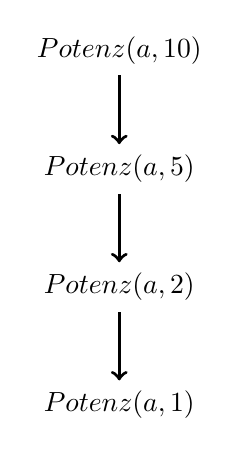
\begin{tikzpicture}[line width=1.2,scale=1.5]
			\node (10) at (0,0) {$\cc{Potenz}(a,10)$};
			\node(5) at (0,-1) {$\cc{Potenz}(a,5)$};
			\node(2) at (0,-2) {$\cc{Potenz}(a,2)$};
			\node(1) at (0,-3) {$\cc{Potenz}(a,1)$};
			\draw[<-]  (1) edge  (2)  (2) edge  (5) (5) edge (10);
		\end{tikzpicture}
	\end{center} 
	Rekursionsbäume mit Verzweigungen erhält man, wenn während der Ausführung einer rekursiven Prozedur mehr als ein rekursiver Aufruf stattfindet. 
\end{bsp} 

\begin{bem}
	Auf der praktischen Seite erfolgt die Umsetzung der Aufrufe von Prozeduren und, insbesondere rekursiven Prozeduren, in Betriebssystemen und Programmiersprachen mit Hilfe des sogenannten Programmstacks. Bei jedem Aufruf wird (intern,auf der Ebene der Maschinensprache) die Stelle im Programm notiert, zu der man nach der Ausführung  der Prozedur zurückkehren soll. Außerdem werden durch einen Aufruf potenziell neue Variablen eingeführt (lokale Variablen der Prozedur, Eingabeparameter). All diese Daten werden auf dem sogenannten \textbf{Aufrufstapel} (engl. call stack, procedure stack) aufgehoben. Die Größe des Aufrufstapels ist standardmäßig ziemlich eingeschränkt, sodass es bei der Ausführung von reksuriven Prozeduren mit einer großen Rekursionstiefe zu einem Überlauf des Aufrufstapels kommen kann. 
	
	In höheren Programmiersprache, bei denen die Rekursion nicht unbedingt direkt durch den Aufrufstapel umgesetzt wird, wird oft trotzdem das Maximum der Rekursionstiefe festgelegt. 	Hier ein Beispiel eines Python-Codes, der diese Problematik illustriert: 
	\lstinputlisting{Code/dive.py}
	
	Auf meinem Computer führt der Aufruf von dive auf der Eingabe $0$ zum eine Stacküberlauf  in der Rekursionstiefe $995$. Die maximale Rekursionstiefe kann oft manuell erhöht werden, und es gibt auch Sprachen, die in gewissen Situationen die rekursiven Prozeduren in nicht-rekursiven Maschinencode übersetzen können. Generell gilt aber: wenn man eine rekursive Prozedur mit einer hohen Rekursionstiefe hat, soll man sich Gedanken darüber machen, wie man diese Prozedur in eine nicht-rekursiv umsetzen könnte. Sehr oft kann man dabei seinen eigenen Stapel anlegen. 
\end{bem} 

\begin{bsp}[Türme von Hanoi] 
	Gegeben sind drei Stäbe: Startstab, Hilfsstab und Zielstab. Auf dem Startstab sind $n$ Scheiben der Größen $1$ bis $n$ aufgestapelt, so dass die Scheiben von oben nach unten betrachtet nach der Größe steigend sortiert sind. Die Rechenaufgabe besteht darin, eine Folge von Schritten zu bestimmen, mit denen man alle $n$ Scheiben vom Startstab auf den Zielstab derart versetzt, dass in jedem Schritt die Scheiben von jedem der drei Stäbe sortiert sind (von oben nach unten betrachtet aufsteigend nach der Größe). 
	
	Eine rekursive Lösung dieser Aufgabe sieht so aus: das Ziel ist $n$ Scheiben vom Start $s$ nach Ziel $z$ mit Hilfe von $h$ als Hilfsstab zu versetzen. Wir versetzen die $n-1$ Scheiben vom Start- auf den Hilfsstab, indem wir das Zielstab als Hilfsstab benutzen. Danach wird die größte Scheibe verfügbar: sie kann auf den Zielstab versetzt werden. Danach ist der Startstab frei und kann bei der Versetzung der $n-1$ Scheiben vom Hilfs- auf den Zielstab als Hilfsstab benutzt werden. 
	
	\begin{algorithm}[H]
	\caption{$\cc{Hanoi-Schritte}(n,s,h,z)$}
	\begin{algorithmic}
		\IF{$n=1$ \COMMENT{Terminierungsbedingung} } 
		\PRINT von $s$ nach $z$ 
		\ELSE
		\STATE $\cc{Hanoi-Schritte}(n-1,s,z,h)$ \COMMENT{alle bis auf die größte Scheibe auf $h$}
		\STATE \COMMENT{Wir verschieben die oberste Scheibe endgültig:} 
		\PRINT von $s$ nach $z$ 
		\STATE  $\cc{Hanoi-Schritte}(n-1,h,s,z)$ \COMMENT{die restlichen $n-1$ Scheiben auf $z$} 
		\ENDIF 
	\end{algorithmic}
\end{algorithm}
	Der Rekursionsbaum für $n=3$ ist wie folgt: 
\begin{center} 
	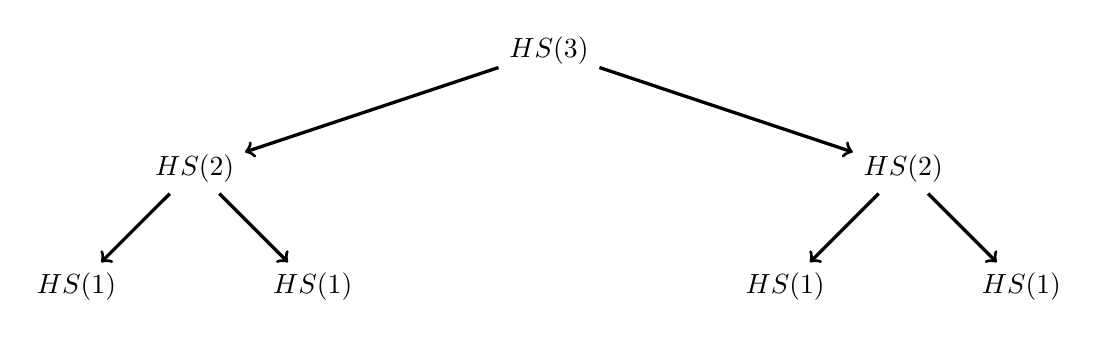
\begin{tikzpicture}[line width=1.2,scale=1.5]
		\node (root) at (0,0) {$\cc{HS}(3)$};
		\node (L) at (-3,-1) {$\cc{HS}(2)$};
		\node (R) at (3,-1) {$\cc{HS}(2)$};
		\node (LL) at (-4,-2)  {$\cc{HS}(1)$};
		\node (LR) at (-2,-2)  {$\cc{HS}(1)$};
		\node (RL) at (2,-2)  {$\cc{HS}(1)$};
		\node (RR) at (4,-2)  {$\cc{HS}(1)$};
		\draw[->]  (root) edge  (L) (root) edge (R) (L) edge (LR) (L) edge (LL) (R) edge (RR) (R) edge (RL);
	\end{tikzpicture}
\end{center} 

	Hierbei steht $\cc{HS}(k)$ für $\cc{Hanoi-Schritte}(k, s,h,z)$ mit irgendeiner Wahl von $s,h,z$. 
	
	Hier Umsetzung in Python mit der Verwendung von Iteratoren: 
\lstinputlisting{Code/hanoi.py}

	Die Demo-Datei für $4$ Türme: \scriptsize{ 
	\url{https://de.wikipedia.org/wiki/T%C3%BCrme_von_Hanoi#/media/Datei:Tower_of_Hanoi_4.gif} } 

\end{bsp} 


\section{Random Access Machine}
\label{sect:RAM}

\begin{bem} 
Die \textbf{Random Access Machine} (kurz \textbf{RAM}), oder auf deutsch, \textbf{Maschine mit wahlfreiem Zugriff}, wird unsere Idealisierung bzw. mathematische Abstraktion des realen Rechners sein. Alle Analysen und Entwürfe von Algorithmen in diesem Kurs werden im Rahmen der RAM durchgeführt. 

Wir nehmen an, dass die Zellen unserer Maschine ganze Zahlen beliebiger Größe speichern können (d.h., die Bit-Größe der Speicherzellen ist unendlich). Die Speichergröße (d.h., die Anzahl der Speicherzellen) ist ebenfalls unbeschränkt (d.h., unendlich). Wir können des Weiteren alle anderen Datentypen auf der Basis der ganzen Zahlen umsetzen. 

Die Random Access Machine kann auch rein formal eingeführt werden. Wir betrachten hier (zunächst) allerdings eine etwas informelle Beschreibung, in der wir festlegen welche Datentypen, Operationen und Kontrollstrukturen für uns elementar sind. 

Als \textbf{Grundoperationen} für unsere RAM erlauben wir:
%
\begin{itemize}
	\item Zuweisung (für ganzzahlige Datentypen)
	\item Addition von ganzzahligen Variablen
	\item Multiplikation einer ganzzahligen Variablen mit einer Konstanten
	\item Ganzzahlige Division einer ganzzahligen Variablen durch eine Konstante
	\item Zugriff zu Speicherzellen über einen Index
	\item Vergleichsoperationen $<$, $\le$, $=$, $\ge$, $>$ 
	\item Kontrollstrukturen if-then-else, while, for 
\end{itemize}

Eine genauere Beschreibung einer RAM findet man bei \cite[Sect.~1.3]{Lov20}.
\end{bem} 

%Unsere Algorithmen werden als Pseudocode formuliert und ihre Analyse wird im Rahmen dieses Modells durchgeführt. Für Pseudocode legen wir fest, dass standardmäßig in Prozeduren alle einfachen Datentypen durch Kopie und alle komplexen Datentypen (Arrays usw.) durch Referenz übergeben werden. 

\begin{bem} 
Wir lassen die Multiplikation von zwei ganzzahligen Variablen in unserem Modell nicht als Grundoperation zu. Denn, wenn das eine Grundoperation wäre, so hätte der folgende Algorithmus die Laufzeit $O(n)$: 

\begin{center}
	\begin{algorithmic}
		\STATE $x:=2$
		\FOR{$i=1,\ldots,n$} 
		\STATE $x:=x^2$
		\ENDFOR
	\end{algorithmic}
\end{center}

Dieser Algorithmus würde also $2^{2^n}$ in der Zeit $O(n)$ berechnen. Die Zahl $2^{2^n}$ hat allerdings $2^n+1$ Binärstellen. Wir würden also eine Zahl exponentieller Bit-Größe in linearer Zeit berechnen, was wir als unrealistisch ansehen. 
\end{bem}

\section{Polynomialzeit-Berechenbarkeit} 



\begin{defn} 
	Sei $A$ Algorithmus im Rahmen eines Rechenmodells, dessen Schritte als Grundoperationen im gegebenen Rechenmodell beschrieben sind. 

Die \textbf{Laufzeit} $L(A,x)$ von~$A$ auf der Eingabeinstanz $x$ ist die Anzahl der Schritte des Algorithmus $A$ auf der Eingabe $x$ bis zur Terminierung. 

Die \textbf{Laufzeitfunktion} $L_A : \N \to \N$ von~$A$ ist definiert als
\[
L_A(n) := \max \setcond{  L(A,x) }{x \ \text{Eingabe für} \ A  \ \text{mit} \ \encl{x} \le n}.
\]
Das heißt, $L_A(n)$ ist die maximale Laufzeit auf allen Eingaben, deren Eingabelänge höchstens $n$ ist. 
\end{defn} 

\begin{defn}
	Eine Funktion $p : \R \to \R$ heißt \textbf{Polynomfunktion} vom Grad $d \in \N_0$, falls~$p$ die Form \[
		p(t)= c_0 + c_1 t + c_2 xt2 + \ldots + c_d t^d
	\]
	hat, mit $c_0,\ldots,c_d \in \R$ und $c_d \ne 0$. 
\end{defn} 

\begin{defn} 
Wir nennen einen Algorithmus~$A$ \textbf{polynomial} oder \textbf{Polynomialzeit-Algorithmus} (bezüglich des zugrundeliegenden Rechenmodells und Kodierungsschemas für die Eingabe), falls eine Polynomfunktion~$p$ existiert, so dass $L_A(n) \leq p(n)$ für alle $n \in \N_0$ gilt.
\end{defn} 

\begin{bem}
	Ein Polynomialzeit-Algorithmus $A$ ist ein Algorithmust mit der Laufzeitfunktion der Ordnung $ O(n^d)$ für ein $d \in \N_0$. 
\end{bem} 

\begin{bem}
	In der Theorie nennt man Polynomialzeit-Algorithmen oft auch effiziente Algorithmen. Welche Algorithmen aus der praktischen Sicht effizient sind, lässt sich schwer formal beschreiben.
\end{bem} 

\begin{defn}
	Ein Rechenproblem heißt \textbf{Polynomialzeit-berechenbar}, wenn es ein Polynomialzeit-Algorithmus existiert, der das Rechenproblem löst. 
	
	Ein Entscheidungsproblem bzw. eine Sprache heißt \textbf{Polynomialzeit-\-ent\-scheid\-bar}, wenn es ein Polynomialzeit-Algorithmus existiert, der das Problem bzw. die Sprache entscheidet. 
\end{defn} 

\begin{defn}
	Die Menge aller Polynomialzeit-entscheidbaren Sprachen $L \subseteq \{0,1\}^\ast$ wird die Komplexitätsklasse $\operatorname{P}$ genannt. Als Formel: 
	\[
			\operatorname{P}:= \setcond{L \subseteq \{0,1\}^\ast }{L \ \text{Polynomialzeit-entscheidbar} } 
	\]
\end{defn} 

 
\chapter{Strukturelle und Algorithmische Graphentheorie} 




\section{Grundbegriffe der Graphentheorie}

\begin{defn}
Sei $V$ eine endliche Menge und sei $A$ eine Teilmenge von $V \times V$.
Das Paar $D=(V,A)$ heißt \emph{Digraph} (engl.~\emph{directed graph}) mit \emph{Knotenmenge} $V$ und \emph{Kantenmenge}~$A$.
Die Elemente von $V$ heißen \emph{Knoten} und die Elemente von $A$ heißen \emph{(gerichtete) Kanten} (engl.~\emph{arcs}) von~$D$.
Ist $(a,b) \in A$ eine \emph{Kante}, so nennen wir~$a$ ihren \emph{Startknoten} und~$b$ ihren \emph{Endkonten}.
Man sagt auch, dass die Knoten $a$ und $b$ \emph{benachbart} und die Kante $(a,b)$ \emph{inzident} zu~$a$ und $b$ ist.
Eine Kante der Form $(a,a)$ heißt \emph{Schlinge}.
\end{defn}

\begin{bsp} 
Digraphen lassen sich auf vielfache Weise anschaulich darstellen.
Eine verbreitete und nützliche Möglichkeit ist das \glqq Zeichnen\grqq\ in die Ebene.
Ein Digraph mit Doppelkante zwischen den Knoten $1$ und $3$ und Schlinge um den Knoten $7$ sei zum Beispiel wie folgt dargestellt:

\begin{center}
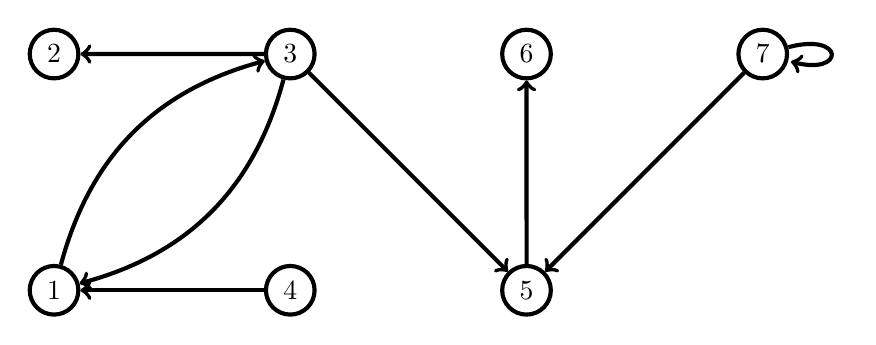
\begin{tikzpicture}[line width=1.5,scale=1.5]
 \node[circle,draw=black] (1) at (0,0) {$1$};
 \node[circle,draw=black] (2) at (0,2) {$2$};
 \node[circle,draw=black] (3) at (2,2) {$3$};
 \node[circle,draw=black] (4) at (2,0) {$4$};
 \node[circle,draw=black] (5) at (4,0) {$5$};
 \node[circle,draw=black] (6) at (4,2) {$6$};
 \node[circle,draw=black] (7) at (6,2) {$7$};
		
 \draw[->] (4) edge (1) (3) edge (2) (3) to[bend left] (1) (3) edge (5) (5) edge (6) (7) edge (5);
 \draw[->] (1) to[bend left] (3) (7) edge[loop right] (7);
\end{tikzpicture}
\end{center}
\end{bsp} 

\begin{defn}
Für einen gegebenen Knoten $a \in V$ heißt die Anzahl der Knoten $b \in V$ mit $(a,b) \in A$ der \emph{Ausgangsgrad} von~$a$.
Analog heißt für $b \in V$ die Anzahl der Knoten $a \in V$ mit $(a,b) \in A$ der \emph{Eingangsgrad} von~$b$.
\end{defn} 

\begin{defn}
Sind $D=(V,A)$ und $D'=(V',A')$ zwei Digraphen, so dass $V' \subseteq V$ und $A' \subseteq A$ gelten, so nennt man $D'$ einen \emph{Teilgraphen} von~$D$.
Ist $W \subseteq V$ so heißt
\[
D_{W} := \left( W, \setcond{(a,b)}{a,b \in W \text{ und } (a,b) \in A} \right)
\]
der durch $W$ \emph{induzierte} Teilgraph von~$D$.
\end{defn}

\begin{defn} 
Für einen Digraphen $D=(V,A)$ und Knoten $a,b \in V$ heißt ein Tupel $(v_0,\ldots,v_k)$ mit $(v_i,v_{i+1}) \in A$, für $0 \leq i \leq k-1$ und $v_0=a$ und $v_k=b$ ein \emph{$(a,b)$-Pfad} der Länge~$k$.
Ein Pfad heißt \emph{Weg}, wenn die Knoten des Pfades paarweise verschieden sind.
Der Pfad $(v_i,\ldots,v_j)$ mit $0 \le i \le j \le k$ heißt \emph{Teilpfad} von $(v_0,\ldots,v_k)$.
Ein $(a,b)$-Pfad mit $a=b$ heißt \emph{Zyklus}.
Ein Zyklus $(v_0,\ldots,v_k)$ heißt \emph{Kreis}, falls die Knoten $v_1,\ldots,v_{k-1}$ paarweise verschieden sind.
Die Zyklen $(v_0,\ldots,v_k)$ und $(v_i,\ldots,v_k,v_0,\ldots,v_i)$ werden als gleich angesehen.
Man sagt eine Kante $(u,v)$ \emph{gehört} zu einem Pfad $(v_0,\ldots,v_k)$, falls $u=v_i$ und $v=v_{i+1}$ für ein $i$ mit $0 \le i \leq k-1$ gilt.
Digraphen ohne Zyklen heißen \emph{azyklisch}.
\end{defn} 

%Seien $G=(V,E)$ und $G=(V',E')$ Digraphen und sei $f: V \to V'$ eine Bijektion mit $(a,b) \in E$ $\Leftrightarrow$ $(f(a), f(b)) \in E'$. Die Bijektion $f$ heißt Isomorphismus von $G$ nach $G'$. Zwei Digraphen heißen isomorph, falls ein Isomorphismus von $G$ nach $G'$ existiert. 

\begin{bsp} 
Im Beispieldigraphen von oben markieren wir den Weg $(4,1,3,5,6)$ in blau:

\begin{center}
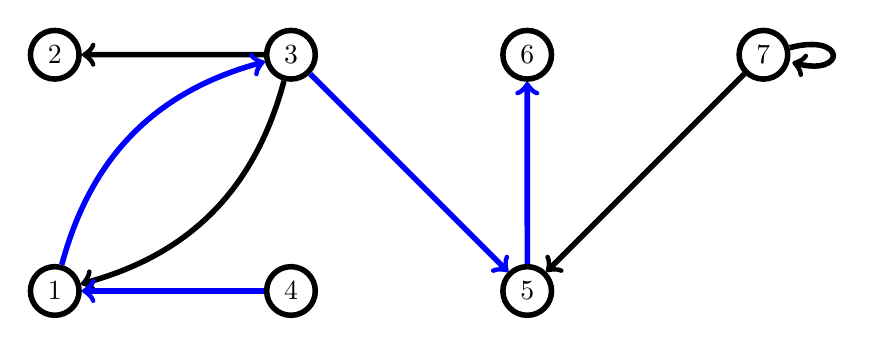
\begin{tikzpicture}[line width=2,scale=1.5]
 \node[circle,draw=black] (1) at (0,0) {$1$};
 \node[circle,draw=black] (2) at (0,2) {$2$};
 \node[circle,draw=black] (3) at (2,2) {$3$};
 \node[circle,draw=black] (4) at (2,0) {$4$};
 \node[circle,draw=black] (5) at (4,0) {$5$};
 \node[circle,draw=black] (6) at (4,2) {$6$};
 \node[circle,draw=black] (7) at (6,2) {$7$};
		
 \draw[->] (3) edge (2) (3) to[bend left] (1) (7) edge (5);
 \draw[->] (7) edge[loop right] (7);
 \draw[->,blue] (4) edge (1) (1) to[bend left] (3) (3) edge (5) (5) edge (6);
 
\end{tikzpicture}
\end{center}
\end{bsp} 

\begin{bem}
Ein wichtiger Aspekt von Digraphen ist die Orientierung der Kanten, die es ermöglicht zwischen Start- und Endknoten zu unterscheiden.
Wird eine solche Orientierung nicht benötigt, so vereinfachen sich manche Begriffe und wir sprechen anstelle von Digraphen dann von Graphen.
\end{bem} 

\begin{defn} 
Sei dazu $V$ wieder eine endliche Menge und sei $E$ nun eine Teilmenge der Menge $\binom{V}{2}= \setcond{\{a,b\}}{a, b \in V, a \ne b} $. 

Das Paar $G=(V,E)$ heißt \emph{Graph} mit \emph{Knotenmenge} $V$ und \emph{Kantenmenge}~$E$.
Die Elemente von $V$ heißen \emph{Knoten} und die Elemente von $E$ heißen \emph{Kanten} (engl.~\emph{edges}) von~$G$.
Ist $\{a,b\} \in E$ eine Kante, so nennen wir~$a$ und~$b$ ihre \emph{Endknoten}.
Wiederum sagen wir, dass die Knoten $a$ und $b$ \emph{benachbart} und die Kante $\{a,b\}$ \emph{inzident} zu~$a$ und $b$ ist.
\end{defn} 

\begin{bem}
Im Gegensatz zu Digraphen erlaubt die Definition eines Graphen keine Schlingen oder parallele Kanten.
In manchen Literaturquellen lässt man mitunter Mehrfachkanten oder \glqq ungerichtete Schlingen\grqq\ zu und spricht dann von einem \emph{einfachen Graphen} wenn man beides verbietet.
\end{bem}

\begin{defn} 
Für einen Knoten $a \in V$ heißt die Anzahl der Knoten $b \in V$ mit $\{a,b\} \in E$ der \emph{Grad} des Knotens~$a$.
Die Begriffe \emph{(induzierter) Teilgraph}, \emph{Pfad}, \emph{Weg}, \emph{Teilpfad}, \emph{Zyklus} und \emph{Kreis} werden für Graphen analog zu denen für Digraphen definiert.
Ein Graph ohne Zyklen heißt \emph{Wald}.
\end{defn}

\begin{defn} 
Ein Graph $G=(V,E)$ heißt \emph{zusammenhängend}, falls für alle Knoten $a, b \in V$ ein $(a,b)$-Pfad existiert.
Ein zusammenhängender Wald heißt \emph{Baum}.
Die Relation \glqq es existiert ein $(a,b)$-Pfad\grqq\ ist eine Äquivalenzrelation auf den Knoten des Graphen~$G$.
Die Äquivalenzklassen bezüglich dieser Relation heißen \emph{Zusammenhangskomponenten} des Graphen.
Ein Wald ist ein Graph bei dem jede Zusammenhangskomponente ein Baum ist.
\end{defn} 


\begin{bsp}
Die folgende Abbildung zeigt einen Graphen mit zwei Zusammenhangskomponenten:

\begin{center}
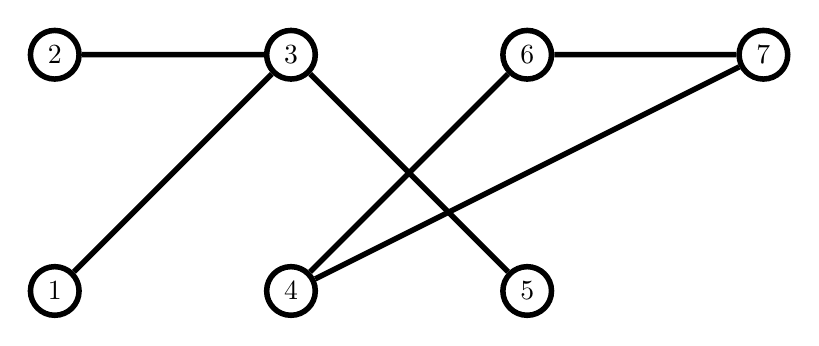
\begin{tikzpicture}[line width=2,scale=1.5]
 \node[circle,draw=black] (1) at (0,0) {$1$};
 \node[circle,draw=black] (2) at (0,2) {$2$};
 \node[circle,draw=black] (3) at (2,2) {$3$};
 \node[circle,draw=black] (4) at (2,0) {$4$};
 \node[circle,draw=black] (5) at (4,0) {$5$};
 \node[circle,draw=black] (6) at (4,2) {$6$};
 \node[circle,draw=black] (7) at (6,2) {$7$};
		
 \draw[-] (3) edge (2) (3) edge (1) (3) edge (5);
 \draw[-] (4) edge (6) (6) edge (7) (7) edge (4);
\end{tikzpicture}
\end{center}
\end{bsp} 

\begin{bem}
Wir benutzen gelegentlich die Kurzbezeichnung $ab:=(a,b)$ für Kanten von Digraphen und $ab:=\{a,b\}$ für Kanten von Graphen.
Beachten Sie, dass es im Fall einer gerichteten Kante auf die Reihenfolge der Knoten~$a$ und $b$ ankommt.
\end{bem}

\begin{defn}
Ein schleifenfreier Digraph $D = (V,A)$ kann auch als Orientierung eines ungerichteten Graphen $G=(V,E)$ mit $E = \{\{u,v\} : (u,v) \in A\}$ verstanden werden.
Der Graph~$G$ wird dann als der \emph{zugrundeliegende Graph} von~$D$ bezeichnet.
Sobald $E$ nicht leer ist, gibt es stets mindestens zwei Digraphen, denen~$G$ zugrundeliegt.
\end{defn} 

\begin{bsp}
Die folgende Abbildung zeigt einen (schleifenfreien) Digraphen und den dazugehörigen zugrundeliegenden Graphen:
\begin{center}
\hfill
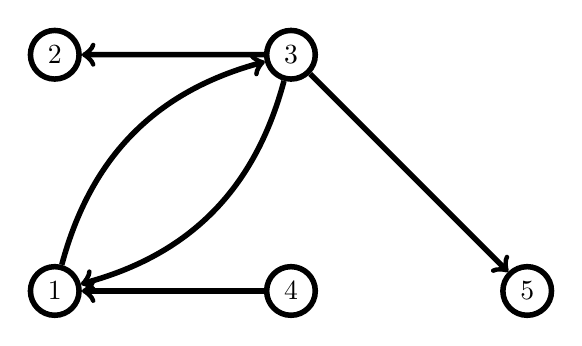
\begin{tikzpicture}[line width=2,scale=1.5]
 \node[circle,draw=black] (1) at (0,0) {$1$};
 \node[circle,draw=black] (2) at (0,2) {$2$};
 \node[circle,draw=black] (3) at (2,2) {$3$};
 \node[circle,draw=black] (4) at (2,0) {$4$};
 \node[circle,draw=black] (5) at (4,0) {$5$};
		
 \draw[->] (4) edge (1) (3) edge (2) (3) to[bend left] (1) (3) edge (5);
 \draw[->] (1) to[bend left] (3);
\end{tikzpicture}
\hfill
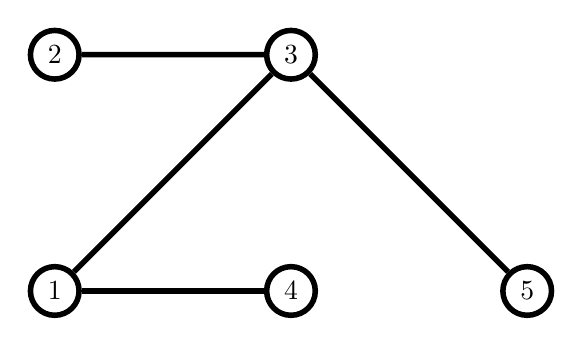
\begin{tikzpicture}[line width=2,scale=1.5]
 \node[circle,draw=black] (1) at (0,0) {$1$};
 \node[circle,draw=black] (2) at (0,2) {$2$};
 \node[circle,draw=black] (3) at (2,2) {$3$};
 \node[circle,draw=black] (4) at (2,0) {$4$};
 \node[circle,draw=black] (5) at (4,0) {$5$};
		
 \draw[-] (1) edge (4) (3) edge (2) (3) edge (1) (3) edge (5);
\end{tikzpicture}
\hfill\,
\end{center}
Beachten Sie, dass die beiden in entgegengesetzten Richtungen orientierten Kanten zwischen den Knoten $1$ und $3$ zu \emph{einer} Kante im ungerichteten Graphen verschmelzen.
\end{bsp}

\begin{defn} 
Halten wir noch ein paar wichtige spezielle Graphenklassen und deren Bezeichnungen fest: Sei dazu im Folgenden $G=(V,E)$ ein Graph mit $n$ Knoten und $m$ Kanten.
\begin{itemize}
 \item Ist $E=\binom{V}{2}$, so heißt $G$ \textbf{vollständig}.
 Ein vollständiger Graph mit $n$ Knoten wird oft mit~$K_n$ bezeichnet.

 \item Ist $E=\emptyset$, so heißt $G$ \textbf{leer}.
 Ein leerer Graph mit $n$ Knoten wird oft mit~$\bar K_n$ bezeichnet.

 \item Ist $V$ eine disjunkte Vereinigung zweier Mengen $A$ und $B$ und hat jede Kante von~$G$ die Form $\{a,b\}$ mit $a \in A$ und $b \in B$, so heißt $G$ \textbf{bipartit}.
 Die Mengen~$A$ und $B$ heißen dann \textbf{Partitionsklassen} von $G$.
 
 \item Ist $G$ bipartit und gilt darüber hinaus, dass jedes $\{a,b\}$ mit $a \in A$ und $b \in B$ eine Kante von $G$ ist, so heißt $G$ \textbf{vollständig bipartit}.
 Ein vollständig bipartiter Graph, deren Partitionsklassen die Größe~$r$ und~$s$ haben, wird oft mit~$K_{r,s}$ bezeichnet.
 Natürlich gilt $n = r + s$.
 
 \item Eine \emph{Einbettung} von~$G$ in die Ebene~$\R^2$ ist eine Menge $P=\{p_1,\ldots,p_n\} \subseteq \R^2$ von Punkten zusammen mit einer Menge $S=\{S_1,\ldots,S_m\}$ von Streckensegmenten, so dass es eine Bijektion $f:V \to P$ gibt mit der Eigenschaft, dass $\{u,v\}$ genau dann eine Kante von~$G$ ist, wenn die Punkte $f(u)$ und $f(v)$ Eckpunkte desselben Streckensegmentes~$S_i$ sind.
 Besitzt ein Graph eine Einbettung bei der je zwei verschiedene Streckensegmente sich höchstens in Eckpunkten schneiden, so heißt dieser Graph \textbf{planar}.
 \end{itemize}
\end{defn} 

\begin{bsp}\
	\begin{itemize} 
	\item  $K_n$ mit $n\leq4$ sind planar. 
	 \item $K_{n,m}$ mit $n \le 2$ und $m \le 3$ sind auch planar. 
	 \item $K_{3,3}$ ist nicht planar. (Beweis durch Widerspruch)
	 \item $K_5$ ist nicht planar. (Beweis durch Widerspruch) 
	 \end{itemize} 
\end{bsp} 

\begin{bsp}
Die nachfolgende Illustration zeigt zwei Darstellungen des $K_4$:
\begin{center}
\hfill
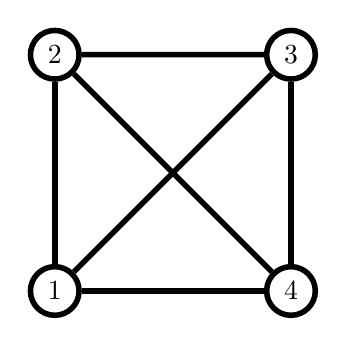
\begin{tikzpicture}[line width=2,scale=1.5]
\tikzset{every loop/.style={}} % no arrows in loops
 \node[circle,draw=black] (1) at (0,0) {$1$};
 \node[circle,draw=black] (2) at (0,2) {$2$};
 \node[circle,draw=black] (3) at (2,2) {$3$};
 \node[circle,draw=black] (4) at (2,0) {$4$};
		
 \draw[-] (1) edge (2) (1) edge (3) (1) edge (4) (2) edge (3) (2) edge (4) (3) edge (4);
		% (4) edge[loop right] (4);		
\end{tikzpicture}
\hfill
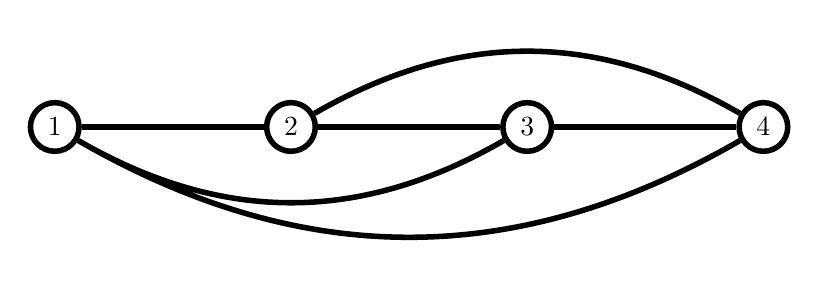
\begin{tikzpicture}[line width=2,scale=1.5]
\tikzset{every loop/.style={}} % no arrows in loops
 \node[circle,draw=black] (1) at (0,0) {$1$};
 \node[circle,draw=black] (2) at (2,0) {$2$};
 \node[circle,draw=black] (3) at (4,0) {$3$};
 \node[circle,draw=black] (4) at (6,0) {$4$};
		
 \draw[-] (1) edge (2) (2) edge (3) (3) edge (4);
 \draw[-] (1) to[bend right] (3) (1) to[bend right] (4);
 \draw[-] (2) to[bend left] (4);		
\end{tikzpicture}
\hfill\,
\end{center}
Keine der beiden Darstellungen zeigt, dass $K_4$ planar ist.
Warum nicht?
Finden Sie eine Darstellung, die dies illustriert!
\end{bsp}

\begin{defn}
	Ein Digraph $D=(V,A)$  heißt \textbf{gerichteter bzgl. gewurzelter Baum} (engl., out-tree oder arborescence) mit Wurzel $w \in V$, wenn der unterichtete Graph zu $D$ ein Baum ist, der Eingangsgrad von $w$ gleich $0$ ist und der Eingangsgrad aller anderen Knoten $v \in V \setminus \{w\}$ gleich $1$ ist. 
\end{defn} 

\begin{prop}
	Zu jedem ungerichteten Baum $G=(V,E)$ und jedem $w \in V$ gibt es genau einen gerichteten Baum zu $G$ mit der Wurzel $w$. 
\end{prop} 
\begin{proof}
	Aufgabe. 
\end{proof} 

\begin{defn}
	Ein Digraph $D=(V,A)$ heißt \textbf{gerichteter Wald}, wenn $V$ disjunkte Vereinigung von Mengen $V_1,\ldots,V_t$ ist, bei denen $D_{V_i}$ für jedes $i=1,\ldots,t$ ein gerichteter Baum ist. 
\end{defn} 

\begin{defn}
	In einem gerichteten Baum/Wald $D=(V,A)$ nennen wir $v \in V$ \textbf{Nachfahre} von $u \in V$ und $u$ \textbf{Vorfahre} von $v$, wenn ein $(u,v)$-Pfad existiert. Wenn $(u,v) \in A$ ist, so nennen wir $v$ \textbf{Kind} oder \textbf{direkter Nachfahre} von $u$ und $u$ \textbf{Vater/Mutter/Elter} von $v$.
\end{defn} 


\begin{bem}
In der Graphentheorie ist die Bezeichnung der Hauptbegriffe nicht einheitlich.
Von Quelle zu Quelle unterscheiden sich die Definitionen geringfügig und insbesondere in Bezug auf die Namensgebung gibt es teilweise große Unterschiede.
Zu diesem Zweck listen wir hier die geläufigsten Synonyme um mögliche Verwirrungen beim Lesen unterschiedlicher Quellen zu vermeiden:
\begin{align*}
\text{gerichteter Graph} &= \text{Digraph}\\
\text{Knoten} &= \text{Ecke}\\
\text{gerichtete Kante} &= \text{Bogen}\\
\text{adjazent} &= \text{benachbart}\\
\text{Grad} &= \text{Valenz}\\
\text{Weg} &= \text{einfacher Pfad}\\
\text{Kreis} &= \text{einfacher Zyklus}\\
\text{Kantenzug} &= \text{Pfad}\\
\text{geschlossener Kantenzug} &= \text{Zyklus}\\
\text{Schleife} &= \text{Schlinge}
\end{align*}
\end{bem}

\section{Speicherung von Graphen} 

\begin{bem}
Zum Abschluss dieser Einführung in die Grundbegriffe schauen wir uns noch verschiedene Möglichkeiten an, wie man einen gegebenen (Di)Graphen im Rechner darstellt, das heißt, in welcher Form man die Beziehungen zwischen Knoten und (gerichteten) Kanten verwalten kann.

Sei dazu ein Graph oder ein Digraph gegeben und zur Vereinheitlichung im Folgenden mit $D=(V,A)$ bezeichnet.
\end{bem} 

\begin{defn}
Die {\bfseries Kantenliste} von $D=(V,A)$ ist die Liste der Kanten von $D$. 
\end{defn}

\begin{bsp}\ 
\begin{center}
\hfill
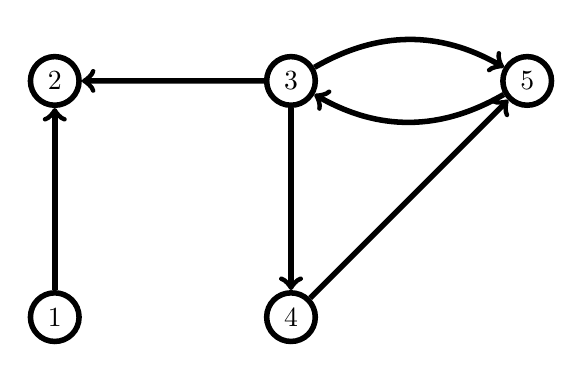
\begin{tikzpicture}[line width=2,scale=1.5]
 \node[circle,draw=black] (1) at (0,0) {$1$};
 \node[circle,draw=black] (2) at (0,2) {$2$};
 \node[circle,draw=black] (3) at (2,2) {$3$};
 \node[circle,draw=black] (4) at (2,0) {$4$};
 \node[circle,draw=black] (5) at (4,2) {$5$};
% \node[black] (G) at (2,3.5) {$G=(V,E)$};
		
 \draw[->] (1) edge (2) (3) edge (2) (3) edge (4) (3) to[bend left] (5) (4) edge (5);
 \draw[->] (5) to[bend left] (3);
\end{tikzpicture}
\hfill
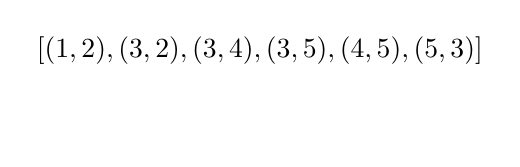
\begin{tikzpicture}[]
 \node[black] (1) at (0,0) {$[ (1,2),(3,2),(3,4),(3,5),(4,5),(5,3) ]$};
 \node[black] (1) at (0,-1) {$ $};
\end{tikzpicture}
\hfill\,
\end{center}
\end{bsp}

\begin{defn} 
In der {\bfseries Adjazenzliste} von $G$ speichert man die Knotenmenge $V$ als Liste und jedem Element $u \in V$ der Liste wird eine Liste aller Knoten $v \in V$ mit $uv \in E$ zugeordnet.
(Der Speicherplatzbedarf für diese Darstellung ist offensichtlich $\Theta(|V|+|E|)$.)
\end{defn}

\begin{bsp} \ 
	\begin{center}
		\hfill
		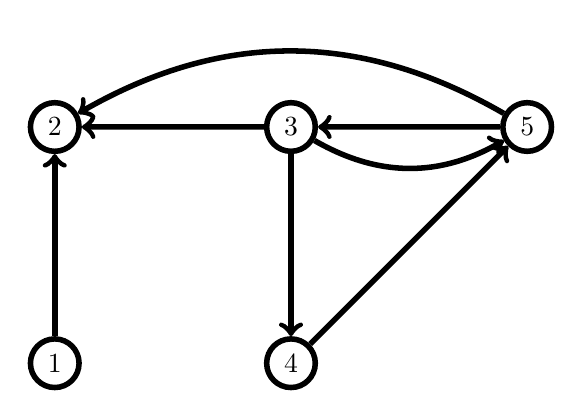
\begin{tikzpicture}[line width=2,scale=1.5]
			\node[circle,draw=black] (1) at (0,0) {$1$};
			\node[circle,draw=black] (2) at (0,2) {$2$};
			\node[circle,draw=black] (3) at (2,2) {$3$};
			\node[circle,draw=black] (4) at (2,0) {$4$};
			\node[circle,draw=black] (5) at (4,2) {$5$};
			% \node[black] (G) at (2,3.5) {$G=(V,E)$};
			
			\draw[->] (1) edge (2) (3) edge (2) (3) edge (4) (3) to[bend right] (5) (4) edge (5);
			\draw[->] (5) edge (3);
			\draw[->] (5) to[bend right] (2);
		\end{tikzpicture}
		\hfill
		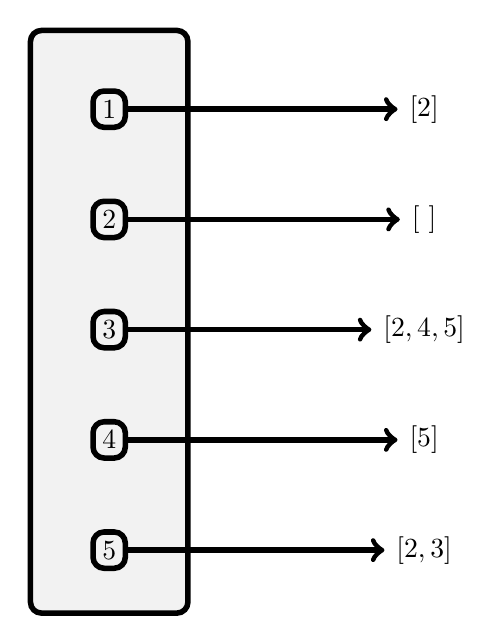
\begin{tikzpicture}[line width=2,scale=2]
			\draw[fill=black!5!white,rounded corners] (-0.5,-3.2) rectangle (0.5,0.5) ;
			\node[rounded corners,draw=black] (1) at (0,0) {$1$};
			\node (L1) at (2,0) {$[2]$};
			\node[rounded corners,draw=black] (2) at (0,-.7) {$2$};
			\node (L2) at (2,-.7) {$[\ ]$};
			\node[rounded corners,draw=black] (3) at (0,-1.4) {$3$};
			\node (L3) at (2,-1.4) {$[2,4,5]$};
			\node[rounded corners,draw=black] (4) at (0,-2.1) {$4$};
			\node (L4) at (2,-2.1) {$[5]$};
			\node[rounded corners,draw=black] (5) at (0,-2.8) {$5$};
			\node (L5) at (2,-2.8) {$[2,3]$};
			
			\draw[->] (1) edge (L1) (2) edge (L2) (3) edge (L3) (4) edge (L4) (5) edge (L5);
		\end{tikzpicture}
		\hfill\,
	\end{center}
\end{bsp} 


\begin{bem}
	Typische Fragen auf Graphen, deren algorithmische Behandlung grundlegend für viele Anwendungen ist, sind zum Beispiel die folgenden:
	\begin{itemize}
		\item Ist der Graph zusammenhängend?
		\item Gibt es einen Pfad im Graphen von einem Knoten $s$ zu einem Knoten $z$?
		\item Wieviele Zusammenhangskomponenten hat der Graph?
		\item Gibt es Kreise oder Zyklen im Graphen?
		\item Was ist der Grad eines gegebenen Knotens?
	\end{itemize}
	
	Ein allgemeines Prinzip um diese Art Fragen zu beantworten ist die sogenannte \emph{Graphendurchmusterung}, deren Ziel es ist alle Knoten und Kanten des gegebenen Graphen zu \glqq erkunden\grqq\ und dabei nützliche Informationen über den Graphen zu sammeln. In Graphendurchmusterungen wird der (Di)Graph in der Regel durch seine Adjazenzliste gegeben. 
\end{bem} 



\begin{defn}
	\textbf{Matrizen} mit $m \in \N$ Zeilen und $n \in \N$ Spalten und mit Komponenten in einer Menge $K$  entsprechen den Abbildungen $A : \{1,\ldots,m\} \times \{1,\ldots,n\} \to K$. Das bedeutet, dass für die Angabe einer Matrix $A$ für alle $i \in \{1,\ldots,m\}$ und $j \in \{1,\ldots,n\}$ die Komponente $A(i,j)$ der Matrix in der Zeile $i$ und Spalte $j$ festgelegt werden muss. 
	
	An der Stelle von $A(i,j)$ benutzt man traditionell eine Bezeichnung mit einem kleinen Buchstaben und untergestellten Indizes $i$ und $j$. 
	
	So schreibt man zum Beispiel
	\[
		A = \bigl (a_{i,j} \bigr)_{\substack{i=1,\ldots,m \\ j=1,\ldots,n}} \in K^{m \times n}
	\]
	wenn man eine Matrix $A$ der Größe $(m,n)$ führen möchte, deren Komponente in der Position $(i,j)$  als $a_{i,j}$ bezeichnet wird. 
\end{defn} 

\begin{defn} 
Sei $|V|=n$ und $V=\{v_1,\ldots,v_n\}$.
Die \textbf{Adjazenzmatrix} von~$G$ ist die Matrix $A=(a_{i,j}) \in \R^{n \times n}$ mit Einträgen
\[
a_{i,j} = \begin{cases}1&,\text{ falls }\{v_i,v_j\} \in E \text{ bzw.~falls }(v_i,v_j) \in E,\\ 0&,\text{ sonst}.\end{cases}
\]
Der Speicherplatzbedarf (bei direkter Implementierung von Matrizen) ist $\Theta(|V|^2)$.
\end{defn} 

\begin{bsp}\
\begin{center}
	\hfill
	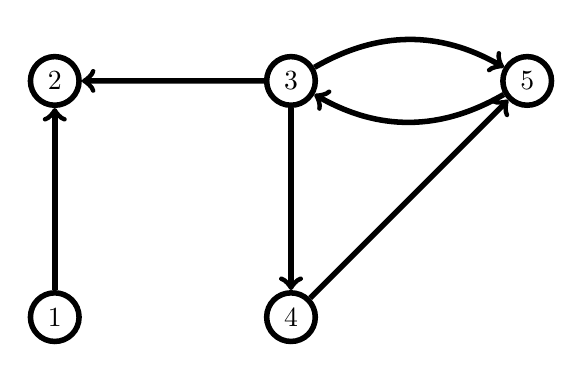
\begin{tikzpicture}[line width=2,scale=1.5]
		\node[circle,draw=black] (1) at (0,0) {$1$};
		\node[circle,draw=black] (2) at (0,2) {$2$};
		\node[circle,draw=black] (3) at (2,2) {$3$};
		\node[circle,draw=black] (4) at (2,0) {$4$};
		\node[circle,draw=black] (5) at (4,2) {$5$};
		% \node[black] (G) at (2,3.5) {$G=(V,E)$};
		
		\draw[->] (1) edge (2) (3) edge (2) (3) edge (4) (3) to[bend left] (5) (4) edge (5);
		\draw[->] (5) to[bend left] (3);
	\end{tikzpicture}
	\hfill
	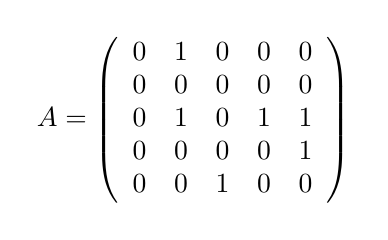
\begin{tikzpicture}[]
		\node[black] (1) at (0,0) {$A=\left(\begin{array}{ccccc}
				0 & 1 & 0 & 0 & 0 \\
				0 & 0 & 0 & 0 & 0 \\
				0 & 1 & 0 & 1 & 1 \\
				0 & 0 & 0 & 0 & 1 \\
				0 & 0 & 1 & 0 & 0
			\end{array}\right)$
		};
	\end{tikzpicture}
	\hfill\,
\end{center}

\end{bsp} 

\begin{defn}
Sei $G=(V,E)$ Digraph mit $m=|E|$ und $n=|V|$ und sei $V=\{v_1,\ldots,v_n\}$ und $E=\{e_1,\ldots,e_m\}$.
Sei weiterhin $G$ zunächst als gerichteter Graph ohne Schleifen angenommen.
Die \textbf{Inzidenzmatrix} von~$G$ ist die Matrix $B=(b_{i,j}) \in \R^{n \times m}$ mit Einträgen
\[
b_{i,j} = \begin{cases}1&,\text{ falls }v_i\text{ Startknoten von }e_j\text{ ist},\\ -1&,\text{ falls }v_i\text{ Endknoten von }e_j\text{ ist},\\ 0&,\text{ sonst}.\end{cases}
\]
Ist $G$ ein ungerichteter Graph, so lassen wir lediglich die Vorzeichen weg, das heißt, die Einträge der Inzidenzmatrix sind
\[
b_{i,j} = \begin{cases}1&,\text{ falls }v_i\text{ Endknoten von }e_j\text{ ist},\\ 0&,\text{ sonst}.\end{cases}
\]
Der Speicherplatzbedarf (bei direkter Implementierung von Matrizen) ist $\Theta(|V|\cdot|E|)$.
\end{defn} 

\begin{bsp} \ 
\begin{center}
\hfill
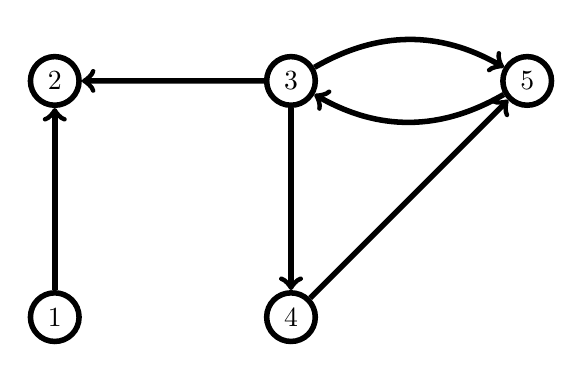
\begin{tikzpicture}[line width=2,scale=1.5]
 \node[circle,draw=black] (1) at (0,0) {$1$};
 \node[circle,draw=black] (2) at (0,2) {$2$};
 \node[circle,draw=black] (3) at (2,2) {$3$};
 \node[circle,draw=black] (4) at (2,0) {$4$};
 \node[circle,draw=black] (5) at (4,2) {$5$};
% \node[black] (G) at (2,3.5) {$G=(V,E)$};
		
 \draw[->] (1) edge (2) (3) edge (2) (3) edge (4) (3) to[bend left] (5) (4) edge (5);
 \draw[->] (5) to[bend left] (3);
\end{tikzpicture}
\hfill
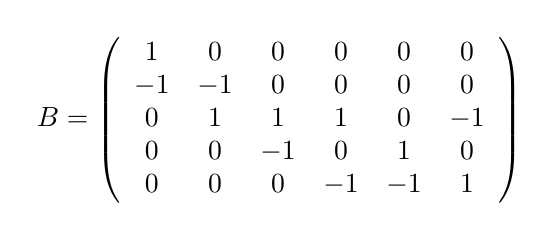
\begin{tikzpicture}[]
 \node[black] (1) at (0,0) {$B=\left(\begin{array}{cccccc}
1 & 0 & 0 & 0 & 0 & 0\\
-1 & -1 & 0 & 0 & 0 & 0\\
0 & 1 & 1 & 1 & 0 & -1\\
0 & 0 & -1 & 0 & 1 & 0\\
0 & 0 & 0 & -1 & -1 & 1
\end{array}\right)$
};
\end{tikzpicture}
\hfill\,
\end{center}

Die Kanten in der vorigen Abbildung sind in der Reihenfolge $12,32,34,35,45,53$ nummeriert.
\end{bsp}  
\section{Tiefensuche}
\label{sect:tiefensuche}


\begin{bem} 
Die Eingabe für die hier diskutierte Tiefensuche ist ein Digraph $D=(V,A)$.
Ist der Graph ungerichtet, so ist die Vorgehensweise vollkommen analog und daher diskutieren wir hier (fast ausschließlich) die gerichtete Variante.
Der Digraph $D$ ist durch seine Adjazenzliste $N$ gegeben, das heißt, für jeden Knoten $u \in V$ ist $N[u]$ eine Liste aller $v \in V$ mit $(u,v) \in A$.
Die Darstellung von $D$ als Adjazenzliste eine Durchmusterung mit der optimalen Laufzeit $\Theta(|V|+|A|)$ erlaubt.
\end{bem}


\begin{bem} 
	Die Tiefensuche ist ein ``reiselustiger'' Algorithmus zur Durchmusterung von Graphen. Wenn wir Knoten als Orte auffassen und $N[u]$ als die Umgebung des Ortes $u$, so können wir das Grundgerüst der Tiefensuche so beschreiben. Man will alle noch nicht gesehenen Orte erkunden, die man von einem gegebenen Ort $u$ aus erreichen kann. Man kann dazu das folgende Vorgehen benutzen: 
	\begin{itemize} 
			\item Man sucht die Umgebung von $u$ durch. 
			\item Sobald man einen  noch nicht besuchten Ort $v$ sieht, erkundet man alle noch nicht gesehene Orte, die man von $v$ aus erreichen kann. 
	\end{itemize} 
	Der Grundgedanke  der Tiefensuche rekursiv: man erkundet neue Orte von $u$ aus, indem man die Orte erkunden, die man aus noch nicht gesehenen Nachbarschaft von $u$ erreichen kann. Die ``Reiselust'' dieser Durchmusterung besteht darin, dass man sich die Erkundung der Orte \emph{sofort} einen neuen Ort versetzt, wenn ein solcher Ort gefunden wird.  
	
	
	Bei rekursiven Algorithmen soll man sich bei der Umsetzung in der Regel als Erstes darum kümmern, dass der Algorithmus terminiert. Daher soll man bei der Durchmusterung die Orte, an die man kommt, gleich als ``gesehen'' markieren.  Stellen Sie sich einfach vor, dass Sie ein Stück Kreide nehmen und da, wo Sie angekommen sind, gleich schreiben ``hier war ich schon''. Sollten Sie bei Ihrer Wanderung durch den Graphen noch ein mal an diesen Ort kommen,  so werden Sie merken, dass Sie an diesem Ort bereits gewesen sind. Auf diese Weise werden Sie nicht endlos im Kreis herumlaufen, wenn etwa Ihr Graph ein Kreis ist oder einen Kreis enthält. 
	
	Die Umsetzung der oben beschriebenen Strategie basiert auf Farbattributen der Knoten, die man im Laufe der Durchmusterung sukzessiv zuerst als weiß ($=$ noch nicht gesehen), dann als  grau ($=$ gesehen aber noch nicht abgearbeitet) und schließlich als  schwarz ($=$ abgearbeitet) setzt. 
\end{bem}

\begin{defn}
	Wenn die Tiefensuche entlang einer Kante verläuft, die in einen weißen Knoten endet, dann sagen wir, dass der entsprechende Knoten \textbf{entdeckt} wird.

Hier eine Zusammenfassung der Bedeutung der Farben der Knoten.  
\begin{itemize}
	\item[] {\bfseries weiß:} Der Knoten wurde noch nicht entdeckt. 
	\item[] {\bfseries grau:} Der Knoten wurde entdeckt und die Tiefensuche für den Knoten läuft gerade.
	\item[] {\bfseries schwarz:} Der Knoten wurde entdeckt und die Tiefensuche für den Knoten ist bereits beendet.
\end{itemize}

Wird ein Knoten schwarz gefärbt, so sagen wir auch das er \textbf{abgearbeitet} wurde.

Durch die Tiefensuche können verschiedene Aufgaben erledigt werden. Nicht alle diese Aufgaben benötigen alle drei Farbattributen der Knoten. Bei manchen Aufgaben reicht auch die Unterscheidung zwischen ``entdeckt'' (weiß) und ``nicht entdeckt'' (grau oder schwarz) aus. 
\end{defn}

\begin{bem}
	Auf diese Weise können wir die Tiefensuche initialisiert: 
	\begin{algorithm} 
		\caption{$\cc{Tiefensuche-Initialisieren}(D)$}
	\begin{algorithmic}[1]
		\FOR{$u \in V$}
		\STATE $\cc{Farbe}[u]=\cc{weiß}$
		\STATE $\pi[u]=\cc{nil}$
		\ENDFOR
		\end{algorithmic}
	\end{algorithm} 
\end{bem}  


\begin{bem} Sobald die Initialisierung erfolgt ist, können wir die Tiefensuche von einem gegebenen Knoten ausführen. Hier die rekursive Umsetzung: 
	\begin{algorithm}[H]
		\caption{$\cc{Tiefensuche}(u)$}
		\begin{algorithmic}[1]
			\STATE $\cc{Farbe}[u]:=\cc{grau}$ \ \COMMENT{$u$ als entdeckt notiert} 
			\FOR{$v \in N[u]$}
			\STATE  \COMMENT{Die Kante $(u,v)$ wird sondiert}
			\IF{$\cc{Farbe}[v]=\cc{weiß}$}
			\STATE $\pi[v]:=u$   \ \COMMENT{Knoten $v$ wurde entdeckt} 
			\STATE $\cc{Tiefensuche}(v)$
			\ENDIF
			\ENDFOR
			\STATE $\cc{Farbe}[u]:=\cc{schwarz}$ 
		\end{algorithmic}
	\end{algorithm}
\end{bem}

\begin{bem} 
	Die Prozedur Tiefensuche können wir in den folgenden Rahmen einbauen. 
	\begin{algorithm}[H]
		\caption{$\cc{Vollständige-Tiefensuche}(D)$}
		\begin{algorithmic}[1]
			\STATE $\cc{Tiefensuche-Initialisieiren}(D)$ 
			\FOR{$u \in V$}\label{line:tiefensuche-hauptschleife-start}
			\IF{$\cc{Farbe}[u]=\cc{weiß}$}
			\STATE $\cc{Tiefensuche}(u)$
			\ENDIF 
			\ENDFOR\label{line:tiefensuche-hauptschleife-ende}
		\end{algorithmic}
	\end{algorithm}
	Durch diese Prozedur entdecken wir jeden jeden Knoten genau ein mal und sondieren dabei jede Kante von $D=(V,A)$. 
\end{bem}




\begin{bem}[Variante mit Zeitstempeln] 
 Jeder Knoten $v \in V$ kann während der Tiefensuche mit zwei \emph{Zeitstempeln} versehen werden: Der erste Zeitstempel $\cc{Grau}[v]$ zeichnet auf, wann der Knoten grau gefärbt wird, das heißt, wann er das erste Mal entdeckt wird.
Der zweite Zeitstempel $\cc{Schwarz}[v]$ hingegen, speichert den Zeitpunkt der Schwarzfärbung von~$v$, das heißt, den Moment in dem der Knoten abgearbeitet ist.

Im Algorithmus werden beide Zeitstempel ganze Zahlen zwischen $1$ und $2 |V|$ sein, da es für jeden Knoten $v \in V$ genau einen Zeitpunkt der Entdeckung (Graufärbung) und einen Zeitpunkt der Abarbeitung (Schwarzfärbung) gibt.

Für jedes $v \in V$ gilt $\cc{Grau}[v] < \cc{Schwarz}[v]$.
Weiterhin ist $v$ vor dem Zeitpunkt $\cc{Grau}[v]$ weiß, während der Zeitpunkte $\cc{Grau}[v],\ldots,\cc{Schwarz}[v]-1$ grau, und ab dem Zeitpunkt $\cc{Schwarz}[v]$ schwarz.

Für die Variante mit den Zeitstempeln sollen die Initialisierung und die Tiefensuche geringfügig ergänzt werden. 

Die Initialisierung: 

	\begin{algorithm} 
	\caption{$\cc{Tiefensuche-Initialisieren}(D)$}
	\begin{algorithmic}[1]
		\FOR{$u \in V$}
		\STATE $\cc{Farbe}[u]=\cc{weiß}$
		\STATE $\pi[u]=\cc{nil}$
		\ENDFOR
		\STATE {\color{red} $t:=0$ \quad \COMMENT{Initialisierung der Zeit-Variablen} }
	\end{algorithmic}
\end{algorithm} 

Die Tiefensuche: 

\begin{algorithm}[H]
	\caption{$\cc{Tiefensuche}(u)$}
	\begin{algorithmic}[1]
		\STATE {\color{red} $t := t + 1$ $\quad$ \COMMENT{Die Uhr tickt vor jeder Färbung} }
		\STATE { \color{red} $\cc{Grau}[u] := t$ $\quad$ \COMMENT{Der Knoten $u$ wurde gerade entdeckt} }
		\STATE $\cc{Farbe}[u]:=\cc{grau}$
		\FOR{$v \in N[u]$}
		\IF{$\cc{Farbe}[v]=\cc{weiß}$}
		 \STATE $\pi[v]:=u$  
		\STATE $\cc{Tiefensuche}(v)$
		\ENDIF
		\ENDFOR
		\STATE {\color{red} $t := t + 1$ $\quad$ \COMMENT{Die Uhr tickt vor jeder Färbung} }
		\STATE\label{line:schwarzfaerbung-in-tiefensuche} {\color{red} $\cc{Schwarz}[u] := t$ $\quad$ \COMMENT{Der Knoten $u$ wurde gerade abgearbeitet}}
		\STATE $\cc{Farbe}[u]:=\cc{schwarz}$
	\end{algorithmic}
\end{algorithm}
\end{bem}

\begin{bsp}
\label{bsp:tiefensuche}
Wir illustrieren die Tiefensuche am Digraphen

\hfill
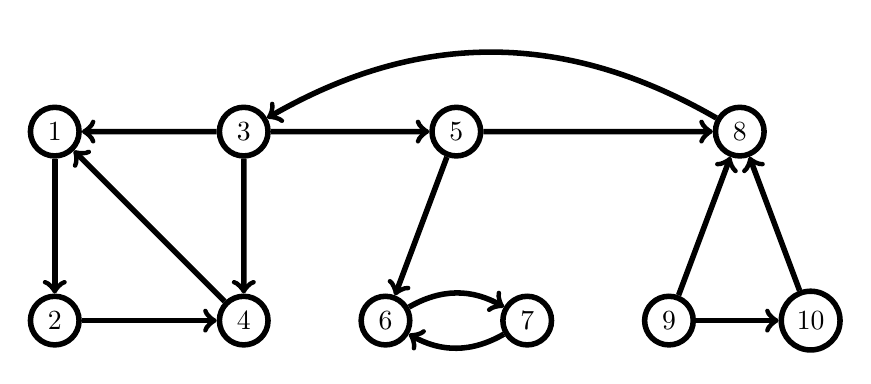
\begin{tikzpicture}[line width=2,scale=1.2]
 \node[circle,draw=black] (1) at (0,2) {$1$};
 \node[circle,draw=black] (2) at (0,0) {$2$};
 \node[circle,draw=black] (3) at (2,2) {$3$};
 \node[circle,draw=black] (4) at (2,0) {$4$};
 \node[circle,draw=black] (5) at (4.25,2) {$5$};
 \node[circle,draw=black] (6) at (3.5,0) {$6$};
 \node[circle,draw=black] (7) at (5,0) {$7$};
 \node[circle,draw=black] (8) at (7.25,2) {$8$};
 \node[circle,draw=black] (9) at (6.5,0) {$9$};
 \node[circle,draw=black] (10) at (8,0) {$10$};
		
 \draw[->] (1) edge (2);
 \draw[->] (2) edge (4);
 \draw[->] (3) edge (1) (3) edge (4) (3) edge (5);
 \draw[->] (4) edge (1);
 \draw[->] (5) edge (6) (5) edge (8); 
 \draw[->] (6) to[bend left] (7);
 \draw[->] (7) to[bend left] (6);
 \draw[->] (8) to[bend right] (3);
 \draw[->] (9) edge (8) (9) edge (10);
 \draw[->] (10) edge (8); 
\end{tikzpicture}
\hfill\,

Wir wählen als Startknoten den Knoten~$3$ und treffen ansonsten jede Wahl aufsteigend in der Reihenfolge der Knotenindizes.
Die ersten sechs Zeitschritte sind durch die folgende Sequenz von gefärbten Digraphen gegeben, wobei die Knotenfarbe dem aktuellen Farbattribut entspricht und die bereits sondierten Kanten rot markiert sind:

\condclearpage 

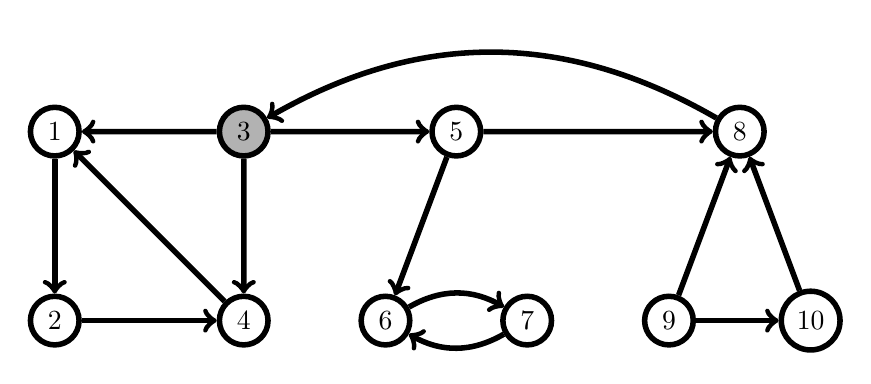
\begin{tikzpicture}[line width=2,scale=1.2]
 \tikzset{gnode/.style ={fill=black!30!,circle,draw}}
 \tikzset{snode/.style ={white,fill=black,circle,draw}}

 \node[circle,draw=black] (1) at (0,2) {$1$};
 \node[circle,draw=black] (2) at (0,0) {$2$};
 \node[gnode] (3) at (2,2) {$3$};
 \node[circle,draw=black] (4) at (2,0) {$4$};
 \node[circle,draw=black] (5) at (4.25,2) {$5$};
 \node[circle,draw=black] (6) at (3.5,0) {$6$};
 \node[circle,draw=black] (7) at (5,0) {$7$};
 \node[circle,draw=black] (8) at (7.25,2) {$8$};
 \node[circle,draw=black] (9) at (6.5,0) {$9$};
 \node[circle,draw=black] (10) at (8,0) {$10$};
		
 \draw[->] (1) edge (2);
 \draw[->] (2) edge (4);
 \draw[->] (3) edge (1) (3) edge (4) (3) edge (5);
 \draw[->] (4) edge (1);
 \draw[->] (5) edge (6) (5) edge (8); 
 \draw[->] (6) to[bend left] (7);
 \draw[->] (7) to[bend left] (6);
 \draw[->] (8) to[bend right] (3);
 \draw[->] (9) edge (8) (9) edge (10);
 \draw[->] (10) edge (8); 
\end{tikzpicture}
\\ $TS(3)$ 

\condclearpage 

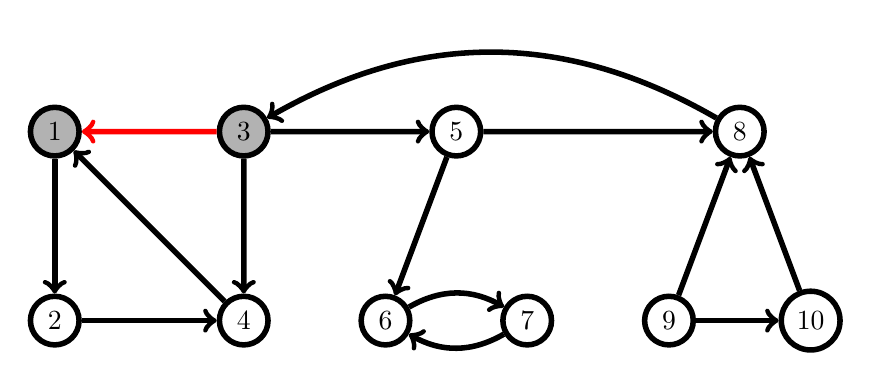
\begin{tikzpicture}[line width=2,scale=1.2]
 \tikzset{gnode/.style ={fill=black!30!,circle,draw}}
 \tikzset{snode/.style ={white,fill=black,circle,draw}}

 \node[gnode] (1) at (0,2) {$1$};
 \node[circle,draw=black] (2) at (0,0) {$2$};
 \node[gnode] (3) at (2,2) {$3$};
 \node[circle,draw=black] (4) at (2,0) {$4$};
 \node[circle,draw=black] (5) at (4.25,2) {$5$};
 \node[circle,draw=black] (6) at (3.5,0) {$6$};
 \node[circle,draw=black] (7) at (5,0) {$7$};
 \node[circle,draw=black] (8) at (7.25,2) {$8$};
 \node[circle,draw=black] (9) at (6.5,0) {$9$};
 \node[circle,draw=black] (10) at (8,0) {$10$};
		
 \draw[->] (1) edge (2);
 \draw[->] (2) edge (4);
 \draw[->,red] (3) edge (1);
 \draw[->] (3) edge (4) (3) edge (5);
 \draw[->] (4) edge (1);
 \draw[->] (5) edge (6) (5) edge (8); 
 \draw[->] (6) to[bend left] (7);
 \draw[->] (7) to[bend left] (6);
 \draw[->] (8) to[bend right] (3);
 \draw[->] (9) edge (8) (9) edge (10);
 \draw[->] (10) edge (8); 
\end{tikzpicture}
\\ $TS(3) \to TS(1)$ 

\condclearpage 
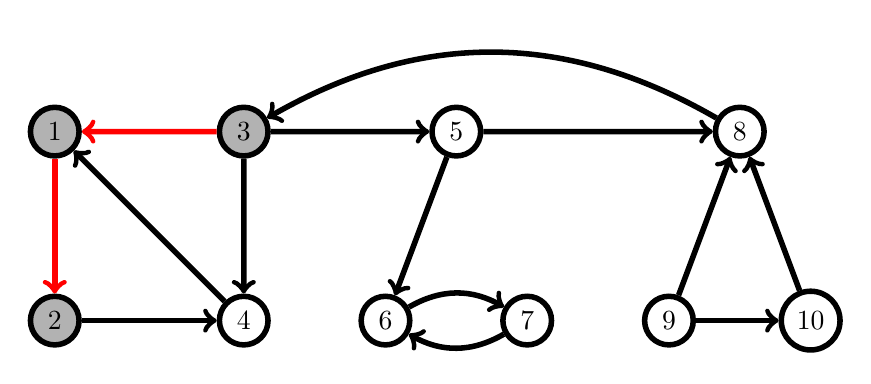
\begin{tikzpicture}[line width=2,scale=1.2]
 \tikzset{gnode/.style ={fill=black!30!,circle,draw}}
 \tikzset{snode/.style ={white,fill=black,circle,draw}}

 \node[gnode] (1) at (0,2) {$1$};
 \node[gnode] (2) at (0,0) {$2$};
 \node[gnode] (3) at (2,2) {$3$};
 \node[circle,draw=black] (4) at (2,0) {$4$};
 \node[circle,draw=black] (5) at (4.25,2) {$5$};
 \node[circle,draw=black] (6) at (3.5,0) {$6$};
 \node[circle,draw=black] (7) at (5,0) {$7$};
 \node[circle,draw=black] (8) at (7.25,2) {$8$};
 \node[circle,draw=black] (9) at (6.5,0) {$9$};
 \node[circle,draw=black] (10) at (8,0) {$10$};
		
 \draw[->,red] (1) edge (2);
 \draw[->] (2) edge (4);
 \draw[->,red] (3) edge (1);
 \draw[->] (3) edge (4) (3) edge (5);
 \draw[->] (4) edge (1);
 \draw[->] (5) edge (6) (5) edge (8); 
 \draw[->] (6) to[bend left] (7);
 \draw[->] (7) to[bend left] (6);
 \draw[->] (8) to[bend right] (3);
 \draw[->] (9) edge (8) (9) edge (10);
 \draw[->] (10) edge (8); 
\end{tikzpicture}
\\ $TS(3)\to TS(1) \to TS(2)$  

\condclearpage 
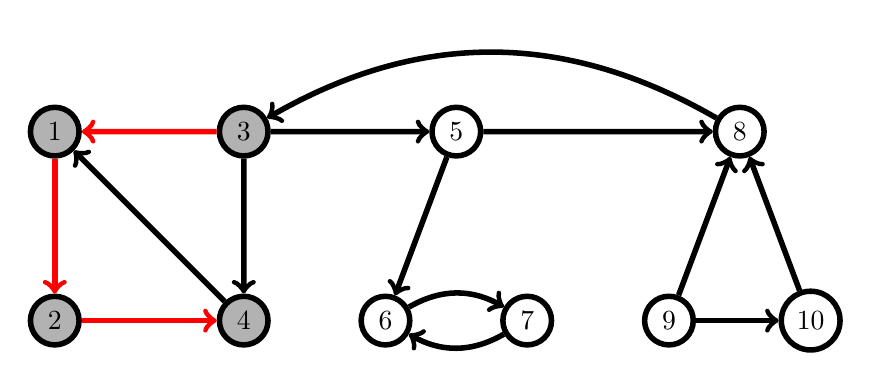
\begin{tikzpicture}[line width=2,scale=1.2]
 \tikzset{gnode/.style ={fill=black!30!,circle,draw}}
 \tikzset{snode/.style ={white,fill=black,circle,draw}}

 \node[gnode] (1) at (0,2) {$1$};
 \node[gnode] (2) at (0,0) {$2$};
 \node[gnode] (3) at (2,2) {$3$};
 \node[gnode] (4) at (2,0) {$4$};
 \node[circle,draw=black] (5) at (4.25,2) {$5$};
 \node[circle,draw=black] (6) at (3.5,0) {$6$};
 \node[circle,draw=black] (7) at (5,0) {$7$};
 \node[circle,draw=black] (8) at (7.25,2) {$8$};
 \node[circle,draw=black] (9) at (6.5,0) {$9$};
 \node[circle,draw=black] (10) at (8,0) {$10$};
		
 \draw[->,red] (1) edge (2);
 \draw[->,red] (2) edge (4);
 \draw[->,red] (3) edge (1);
 \draw[->] (3) edge (4) (3) edge (5);
 \draw[->] (4) edge (1);
 \draw[->] (5) edge (6) (5) edge (8); 
 \draw[->] (6) to[bend left] (7);
 \draw[->] (7) to[bend left] (6);
 \draw[->] (8) to[bend right] (3);
 \draw[->] (9) edge (8) (9) edge (10);
 \draw[->] (10) edge (8); 
\end{tikzpicture}
\\ $TS(3)\to TS(1) \to TS(2) \to TS(4)$ 

\condclearpage
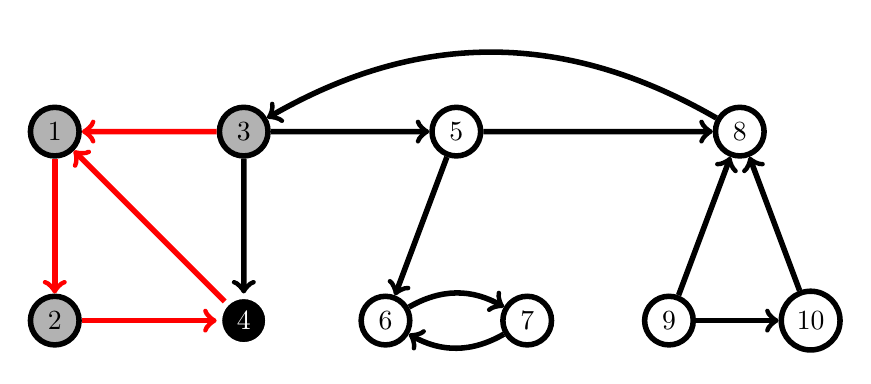
\begin{tikzpicture}[line width=2,scale=1.2]
 \tikzset{gnode/.style ={fill=black!30!,circle,draw}}
\tikzset{snode/.style ={white,fill=black,circle,draw}}

 \node[gnode] (1) at (0,2) {$1$};
 \node[gnode] (2) at (0,0) {$2$};
 \node[gnode] (3) at (2,2) {$3$};
 \node[snode] (4) at (2,0) {$4$};
 \node[circle,draw=black] (5) at (4.25,2) {$5$};
 \node[circle,draw=black] (6) at (3.5,0) {$6$};
 \node[circle,draw=black] (7) at (5,0) {$7$};
 \node[circle,draw=black] (8) at (7.25,2) {$8$};
 \node[circle,draw=black] (9) at (6.5,0) {$9$};
 \node[circle,draw=black] (10) at (8,0) {$10$};
		
 \draw[->,red] (1) edge (2);
 \draw[->,red] (2) edge (4);
 \draw[->,red] (3) edge (1);
 \draw[->] (3) edge (4) (3) edge (5);
 \draw[->,red] (4) edge (1);
 \draw[->] (5) edge (6) (5) edge (8); 
 \draw[->] (6) to[bend left] (7);
 \draw[->] (7) to[bend left] (6);
 \draw[->] (8) to[bend right] (3);
 \draw[->] (9) edge (8) (9) edge (10);
 \draw[->] (10) edge (8); 
\end{tikzpicture}
\\ $TS(3)\to TS(1) \to TS(2)$

\condclearpage 
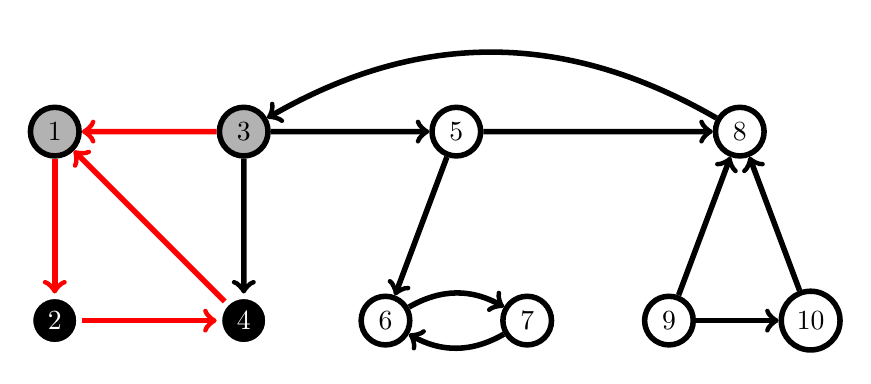
\begin{tikzpicture}[line width=2,scale=1.2]
 \tikzset{gnode/.style ={fill=black!30!,circle,draw}}
 \tikzset{snode/.style ={white,fill=black,circle,draw}}

 \node[gnode] (1) at (0,2) {$1$};
 \node[snode] (2) at (0,0) {$2$};
 \node[gnode] (3) at (2,2) {$3$};
 \node[snode] (4) at (2,0) {$4$};
 \node[circle,draw=black] (5) at (4.25,2) {$5$};
 \node[circle,draw=black] (6) at (3.5,0) {$6$};
 \node[circle,draw=black] (7) at (5,0) {$7$};
 \node[circle,draw=black] (8) at (7.25,2) {$8$};
 \node[circle,draw=black] (9) at (6.5,0) {$9$};
 \node[circle,draw=black] (10) at (8,0) {$10$};
		
 \draw[->,red] (1) edge (2);
 \draw[->,red] (2) edge (4);
 \draw[->,red] (3) edge (1);
 \draw[->] (3) edge (4) (3) edge (5);
 \draw[->,red] (4) edge (1);
 \draw[->] (5) edge (6) (5) edge (8); 
 \draw[->] (6) to[bend left] (7);
 \draw[->] (7) to[bend left] (6);
 \draw[->] (8) to[bend right] (3);
 \draw[->] (9) edge (8) (9) edge (10);
 \draw[->] (10) edge (8); 
\end{tikzpicture}
\\ $TS(3)\to TS(1)$

Wir steigen zum Zeitpunkt $\cc{Schwarz}[8]=14$ mit der Illustration wieder ein:

\condclearpage 
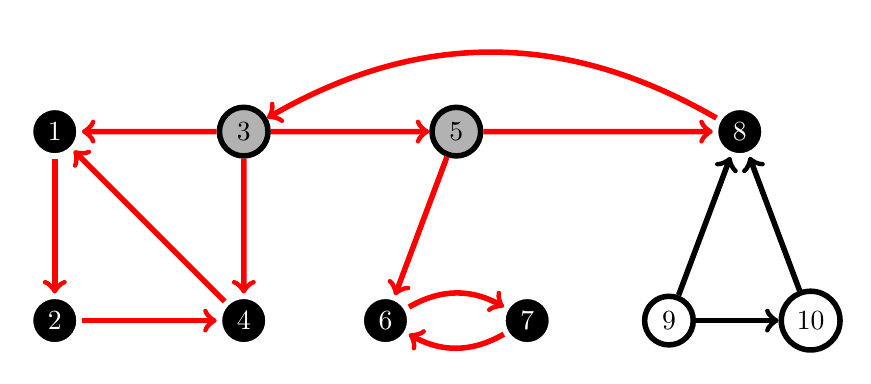
\begin{tikzpicture}[line width=2,scale=1.2]
 \tikzset{gnode/.style ={fill=black!30!,circle,draw}}
 \tikzset{snode/.style ={white,fill=black,circle,draw}}

 \node[snode] (1) at (0,2) {$1$};
 \node[snode] (2) at (0,0) {$2$};
 \node[gnode] (3) at (2,2) {$3$};
 \node[snode] (4) at (2,0) {$4$};
 \node[gnode] (5) at (4.25,2) {$5$};
 \node[snode] (6) at (3.5,0) {$6$};
 \node[snode] (7) at (5,0) {$7$};
 \node[snode] (8) at (7.25,2) {$8$};
 \node[circle,draw=black] (9) at (6.5,0) {$9$};
 \node[circle,draw=black] (10) at (8,0) {$10$};
		
 \draw[->,red] (1) edge (2);
 \draw[->,red] (2) edge (4);
 \draw[->,red] (3) edge (1);
 \draw[->,red] (3) edge (4) (3) edge (5);
 \draw[->,red] (4) edge (1);
 \draw[->,red] (5) edge (6) (5) edge (8); 
 \draw[->,red] (6) to[bend left] (7);
 \draw[->,red] (7) to[bend left] (6);
 \draw[->,red] (8) to[bend right] (3);
 \draw[->] (9) edge (8) (9) edge (10);
 \draw[->] (10) edge (8); 
\end{tikzpicture}
\\ $TS(3)\to TS(5)$

\condclearpage 
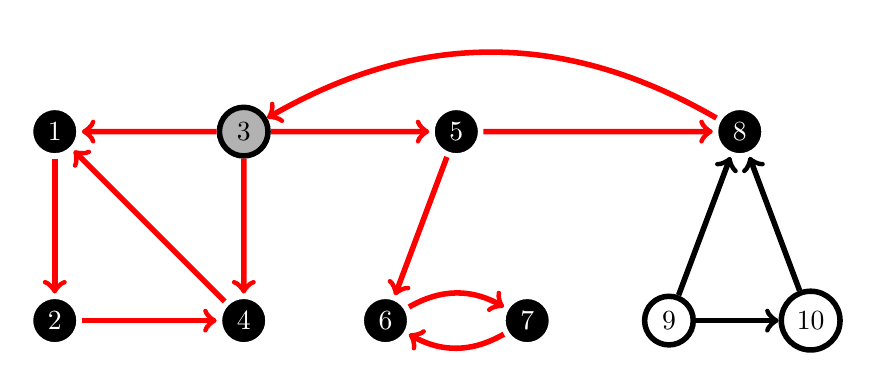
\begin{tikzpicture}[line width=2,scale=1.2]
 \tikzset{gnode/.style ={fill=black!30!,circle,draw}}
 \tikzset{snode/.style ={white,fill=black,circle,draw}}

 \node[snode] (1) at (0,2) {$1$};
 \node[snode] (2) at (0,0) {$2$};
 \node[gnode] (3) at (2,2) {$3$};
 \node[snode] (4) at (2,0) {$4$};
 \node[snode] (5) at (4.25,2) {$5$};
 \node[snode] (6) at (3.5,0) {$6$};
 \node[snode] (7) at (5,0) {$7$};
 \node[snode] (8) at (7.25,2) {$8$};
 \node[circle,draw=black] (9) at (6.5,0) {$9$};
 \node[circle,draw=black] (10) at (8,0) {$10$};
		
 \draw[->,red] (1) edge (2);
 \draw[->,red] (2) edge (4);
 \draw[->,red] (3) edge (1);
 \draw[->,red] (3) edge (4) (3) edge (5);
 \draw[->,red] (4) edge (1);
 \draw[->,red] (5) edge (6) (5) edge (8); 
 \draw[->,red] (6) to[bend left] (7);
 \draw[->,red] (7) to[bend left] (6);
 \draw[->,red] (8) to[bend right] (3);
 \draw[->] (9) edge (8) (9) edge (10);
 \draw[->] (10) edge (8); 
\end{tikzpicture}
\hfill\,

\condclearpage 
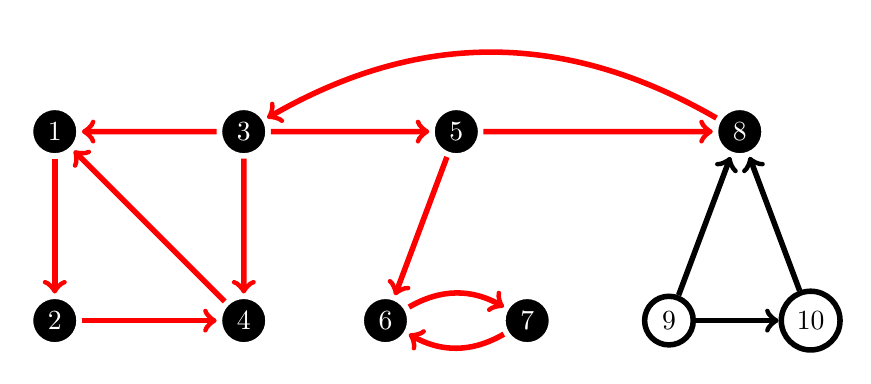
\begin{tikzpicture}[line width=2,scale=1.2]
 \tikzset{gnode/.style ={fill=black!30!,circle,draw}}
 \tikzset{snode/.style ={white,fill=black,circle,draw}}

 \node[snode] (1) at (0,2) {$1$};
 \node[snode] (2) at (0,0) {$2$};
 \node[snode] (3) at (2,2) {$3$};
 \node[snode] (4) at (2,0) {$4$};
 \node[snode] (5) at (4.25,2) {$5$};
 \node[snode] (6) at (3.5,0) {$6$};
 \node[snode] (7) at (5,0) {$7$};
 \node[snode] (8) at (7.25,2) {$8$};
 \node[circle,draw=black] (9) at (6.5,0) {$9$};
 \node[circle,draw=black] (10) at (8,0) {$10$};
		
 \draw[->,red] (1) edge (2);
 \draw[->,red] (2) edge (4);
 \draw[->,red] (3) edge (1);
 \draw[->,red] (3) edge (4) (3) edge (5);
 \draw[->,red] (4) edge (1);
 \draw[->,red] (5) edge (6) (5) edge (8); 
 \draw[->,red] (6) to[bend left] (7);
 \draw[->,red] (7) to[bend left] (6);
 \draw[->,red] (8) to[bend right] (3);
 \draw[->] (9) edge (8) (9) edge (10);
 \draw[->] (10) edge (8); 
\end{tikzpicture}
\hfill\,

Nun muss ein neuer Knoten gewählt werden (Knoten $9$) um die Tiefensuche für den ganzen Digraphen zu beenden:

\condclearpage 
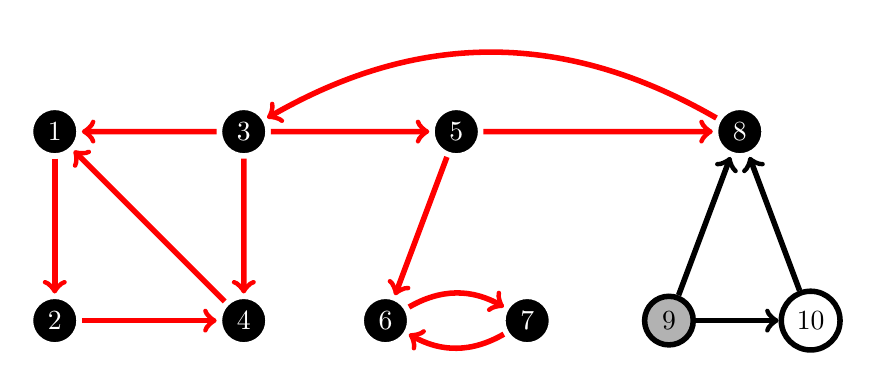
\begin{tikzpicture}[line width=2,scale=1.2]
 \tikzset{gnode/.style ={fill=black!30!,circle,draw}}
 \tikzset{snode/.style ={white,fill=black,circle,draw}}

 \node[snode] (1) at (0,2) {$1$};
 \node[snode] (2) at (0,0) {$2$};
 \node[snode] (3) at (2,2) {$3$};
 \node[snode] (4) at (2,0) {$4$};
 \node[snode] (5) at (4.25,2) {$5$};
 \node[snode] (6) at (3.5,0) {$6$};
 \node[snode] (7) at (5,0) {$7$};
 \node[snode] (8) at (7.25,2) {$8$};
 \node[gnode] (9) at (6.5,0) {$9$};
 \node[circle,draw=black] (10) at (8,0) {$10$};
		
 \draw[->,red] (1) edge (2);
 \draw[->,red] (2) edge (4);
 \draw[->,red] (3) edge (1);
 \draw[->,red] (3) edge (4) (3) edge (5);
 \draw[->,red] (4) edge (1);
 \draw[->,red] (5) edge (6) (5) edge (8); 
 \draw[->,red] (6) to[bend left] (7);
 \draw[->,red] (7) to[bend left] (6);
 \draw[->,red] (8) to[bend right] (3);
 \draw[->] (9) edge (8) (9) edge (10);
 \draw[->] (10) edge (8); 
\end{tikzpicture}
\hfill\,

\condclearpage 
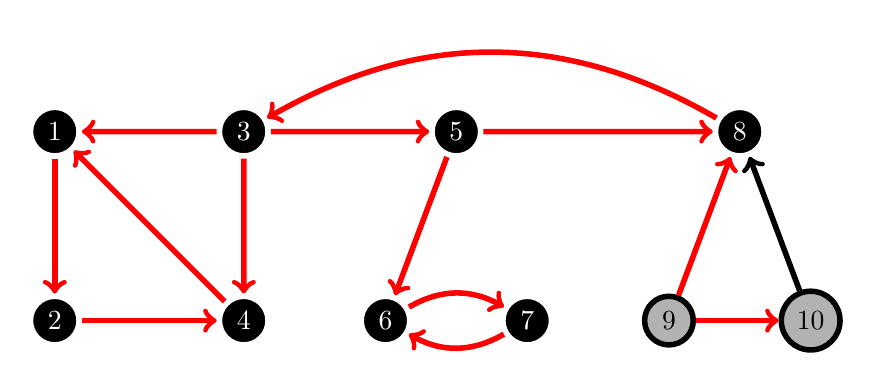
\begin{tikzpicture}[line width=2,scale=1.2]
 \tikzset{gnode/.style ={fill=black!30!,circle,draw}}
 \tikzset{snode/.style ={white,fill=black,circle,draw}}

 \node[snode] (1) at (0,2) {$1$};
 \node[snode] (2) at (0,0) {$2$};
 \node[snode] (3) at (2,2) {$3$};
 \node[snode] (4) at (2,0) {$4$};
 \node[snode] (5) at (4.25,2) {$5$};
 \node[snode] (6) at (3.5,0) {$6$};
 \node[snode] (7) at (5,0) {$7$};
 \node[snode] (8) at (7.25,2) {$8$};
 \node[gnode] (9) at (6.5,0) {$9$};
 \node[gnode] (10) at (8,0) {$10$};
		
 \draw[->,red] (1) edge (2);
 \draw[->,red] (2) edge (4);
 \draw[->,red] (3) edge (1);
 \draw[->,red] (3) edge (4) (3) edge (5);
 \draw[->,red] (4) edge (1);
 \draw[->,red] (5) edge (6) (5) edge (8); 
 \draw[->,red] (6) to[bend left] (7);
 \draw[->,red] (7) to[bend left] (6);
 \draw[->,red] (8) to[bend right] (3);
 \draw[->,red] (9) edge (8) (9) edge (10);
 \draw[->] (10) edge (8); 
\end{tikzpicture}
\hfill\,

\condclearpage 
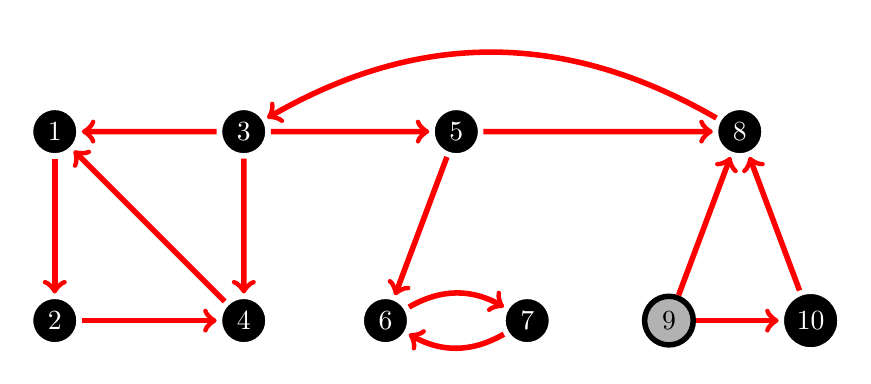
\begin{tikzpicture}[line width=2,scale=1.2]
 \tikzset{gnode/.style ={fill=black!30!,circle,draw}}
 \tikzset{snode/.style ={white,fill=black,circle,draw}}

 \node[snode] (1) at (0,2) {$1$};
 \node[snode] (2) at (0,0) {$2$};
 \node[snode] (3) at (2,2) {$3$};
 \node[snode] (4) at (2,0) {$4$};
 \node[snode] (5) at (4.25,2) {$5$};
 \node[snode] (6) at (3.5,0) {$6$};
 \node[snode] (7) at (5,0) {$7$};
 \node[snode] (8) at (7.25,2) {$8$};
 \node[gnode] (9) at (6.5,0) {$9$};
 \node[snode] (10) at (8,0) {$10$};
		
 \draw[->,red] (1) edge (2);
 \draw[->,red] (2) edge (4);
 \draw[->,red] (3) edge (1);
 \draw[->,red] (3) edge (4) (3) edge (5);
 \draw[->,red] (4) edge (1);
 \draw[->,red] (5) edge (6) (5) edge (8); 
 \draw[->,red] (6) to[bend left] (7);
 \draw[->,red] (7) to[bend left] (6);
 \draw[->,red] (8) to[bend right] (3);
 \draw[->,red] (9) edge (8) (9) edge (10);
 \draw[->,red] (10) edge (8); 
\end{tikzpicture}
\hfill\,

\condclearpage 
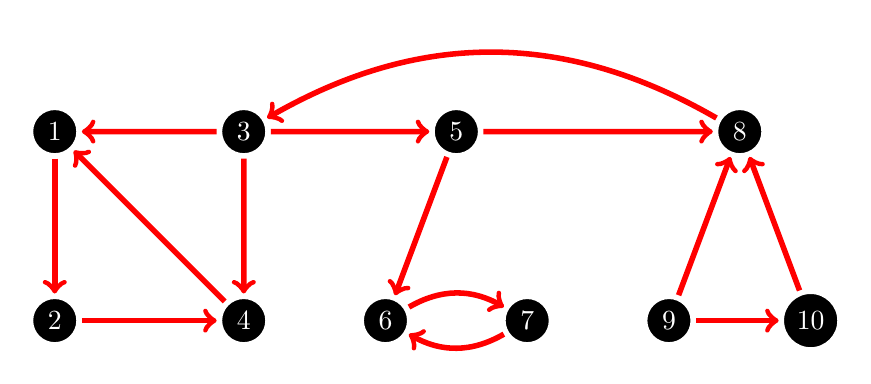
\begin{tikzpicture}[line width=2,scale=1.2]
 \tikzset{gnode/.style ={fill=black!30!,circle,draw}}
 \tikzset{snode/.style ={white,fill=black,circle,draw}}

 \node[snode] (1) at (0,2) {$1$};
 \node[snode] (2) at (0,0) {$2$};
 \node[snode] (3) at (2,2) {$3$};
 \node[snode] (4) at (2,0) {$4$};
 \node[snode] (5) at (4.25,2) {$5$};
 \node[snode] (6) at (3.5,0) {$6$};
 \node[snode] (7) at (5,0) {$7$};
 \node[snode] (8) at (7.25,2) {$8$};
 \node[snode] (9) at (6.5,0) {$9$};
 \node[snode] (10) at (8,0) {$10$};
		
 \draw[->,red] (1) edge (2);
 \draw[->,red] (2) edge (4);
 \draw[->,red] (3) edge (1);
 \draw[->,red] (3) edge (4) (3) edge (5);
 \draw[->,red] (4) edge (1);
 \draw[->,red] (5) edge (6) (5) edge (8); 
 \draw[->,red] (6) to[bend left] (7);
 \draw[->,red] (7) to[bend left] (6);
 \draw[->,red] (8) to[bend right] (3);
 \draw[->,red] (9) edge (8) (9) edge (10);
 \draw[->,red] (10) edge (8); 
\end{tikzpicture}
\hfill\,

Nun sind alle Knoten schwarz und die Tiefensuche ist beendet.
\end{bsp}

%Als Beispiel kann man die TS mit dem Startknoten $1$ im Fall von $N$:
%\[
%	\begin{array}{llll}
%	1: & 2, & 4 
%	\\ 2: & 3
%	\\ 3: & 
%	\\ 4: & 2, & 3, & 5
%	\\ 5: & 6
%	\\ 6: & 4
%	\\ 7: & 6
%	\end{array}
%\]
%betrachten. Wir protokollieren die Änderungen wann welche TSen aufgerufen und beendet werden und wie sich die Farben der Knoten ändern. *****

\begin{bem}
	Bevor wir die Anwendungen der Tiefensuche diskutieren, analysieren wir Ihre Laufzeit. 
\end{bem} 

\begin{thm}
\label{thm:laufzeit-tiefensuche}
Es sei ein Digraph $D=(V,A)$ durch eine Adjazenzliste gegeben. Dann hat die Laufzeit von $\cc{Tiefensuche}(s)$ die Ordnung $O(|V|+|A|)$ und die  Laufzeit von $\cc{Vollständige-Tiefensuche}(D)$ die Ordnung $\Theta(|V|+|A|)$.
\end{thm}

\begin{proof}
Der Aufwand setzt sich aus aus den folgenden Operationen zusammen, die man den Knoten und Kanten zuordnet: 

\begin{equation*}
	\cc{weiss} 
	\ \xrightarrow{\text{$TS(u)$ Start}} \ 
	\cc{grau}
	\ \xrightarrow{\text{Sondierung von $N[u]$}}
	\ \cc{schwarz} 
	\  \xrightarrow{\text{$TS(u)$ Ende}} \ 
\end{equation*} 

Hier wird $TS$ als Abkürzung für $\cc{Tiefensuche}$ benutzt. Für die Tiefensuche und vollständige Tiefensuche ist der Aufwand somit höchstens $O(|V|+|E|)$, denn der Aufwand pro Konten  $O(1)$, da kein Knoten $u$ wegen der Änderung der Farben mehr als ein mal sondiert werden kann. Genau so ist der Aufwand pro jede Kante $O(1)$, da eine Kante $(u,v)$ genau dann sondiert wird, wenn man $u$ entdeckt, der Knoten $u$ wird aber höchstens ein mal entdeckt. 

Es ist klar, dass der Aufwand bei der vollständigen Tiefensuche $\Omega(|V|+|A|)$, da die For-Schleife in der vollständige Tiefensuche dafür sorgt, dass jeder Knoten ein mal entdeckt wird. 
\end{proof}


%\begin{thm}
%	Sei $G=(V,E)$ Digraph mit $m \in \N$ Kanten und $n \in \N$ Knoten, der durch eine Adjazenzliste gegeben ist. Sei $s \in V$. Dan gilt für die Tiefensuche auf $G$ mit dem Startknoten $s$:
%	\begin{enumerate}[(a)]
%		\item Die Laufzeit des Verfahrens ist $O(m+n)$ (das heißt, höchstens $c(m+n)$ für eine Konstante $c>0$).
%		\item Die Menge aller Knoten von $G$, die von $s$ aus durch einen Pfad erreichbar sind ist genau die Menge der Knoten, die während der Ausführung entdeckt werden. 
%		\item Der Graph $G$ enthält genau dann einen von $s$ aus erreichbaren Zyklus, wenn während der Ausführung beim Sondieren einer der Kanten $(u,v)$ die Farbe von $v$ grau ist. 
%	\end{enumerate} 
%\end{thm}
%\begin{proof}
%	(a): Während der Ausführung werden die folgende Operationen ausgeführt: Änderung der Farben und Aufruf der TS für unterschiedliche Knoten sowie Sondierung der Kanten. Jeder entdeckte Knoten ändert seine Farbe von weiß zu grau und anschließend zu schwarz. Da eine TS nur für einen weißen Knoten gestartet wird, wird die TS für jeden Knoten höchstens ein mal ausgeführt. Somit dauert die Bearbeitung von jedem Knoten (Farbenänderung, Aufruf der TS) $O(1)$ Zeiteinheiten. Eine Kante $(u,v)$ wird genau dann sondiert, wenn die TS für $u$ aufgerufen wird. Somit kann jede Kante höchstens ein mal sondiert werden. Das Sondieren jeder Kante beträgt dadurch höchstens $O(1)$ Zeiteinheiten. Der Gesamtaufwand der TS mit dem Startknoten $s$ ist somit $O(m+n)$. 
%	
%	(b): Seien $u_1,\ldots,u_k$ alle Knoten, die während der Ausführung entdeckt werden und seien $u_1,\ldots,u_k$ in dieser Reihenfolge entdeckt ($u_1$ ist der erste entdeckte Knoten, $u_2$ der zweite usw.). Dann ist $u_1$ von $s$ aus erreichbar, denn $u_1=s$. Die TS für einen Knoten $u_j$ mit $j > 1$ wird aus einer TS für einen Knoten $u_i$ aufgerufen, der im Moment der Aufuruf von $TS(u_j)$ bereits entdeckt ist. Man hat also $j< i$. Wenn $u_j$ von $s$ aus erreichbar ist, so ist auch $u_i$ von $s$ aus erreichbar, da $(u_i,u_j)$ eine Kante von $G$ ist. Somit folgt durch Induktion über $j$, das jeder Knoten $u_j$ von $s$ aus erreichbar ist. 
%	
%	Umgekehrt zeigen wir nun, dass jeder Knoten $v \in V$, der von $s$ aus erreichbar ist, während der Ausführung entdeckt wird. Sei $(v_0,\ldots,v_k)$ ein Pfad von $s$ nach $v$. Wir zeigen nun, dass jeder Knoten $v_j$ dieses Pfades entdeckt wird. Für $v_0=s$ gilt die Aussage offensichtlich. Wird ein Knoten $v_j$ mit $j < k$ entdeckt, so entdeckt man den Knoten $v_{j+1}$ spätestens beim Sondieren der Kante $(v_j,v_{j+1})$ innerhalb der TS für $v_j$. Es kann als durch Induktion über $j$ gezeigt werden, dass alle $v_j$ und insbesondere auch $v_k=v$ entdeckt werden.
%	
%	(c): Der Beweis von (c) ist analog zum Beweis von (b) und wird hier nicht angeführt. (Aufgabe)
%\end{proof}
%

\begin{defn} 
Die Vorgängerabbildung $\pi$ erzeugt den sogenannten \textbf{Vor\-gänger\-teil\-graphen} eines Digraphen $D=(V,A)$, der formal durch $D_\pi=(V,A_\pi)$ mit
\[
A_\pi = \left\{(\pi[v],v) : v \in V \text{ und } \pi[v] \neq \cc{nil}\right\}
\]
definiert ist.
Für jede Tiefensuche ist der Vorgängerteilgraph ein Wald, und wird daher im Folgenden als \textbf{Tiefensuchwald} bezeichnet.
Er ist aus einem oder mehreren \textbf{Tiefensuchbäumen} zusammengesetzt.
\end{defn} 

\begin{bsp} 
In Beispiel~\ref{bsp:tiefensuche} ist die Vorgängerabbildung nach abgeschlossener Tiefensuche durch $\pi=[3,1,\cc{nil},2,3,5,6,5,\cc{nil},9]$ gegeben.
Der zugehörige Tiefensuchwald ist also

\begin{center} 
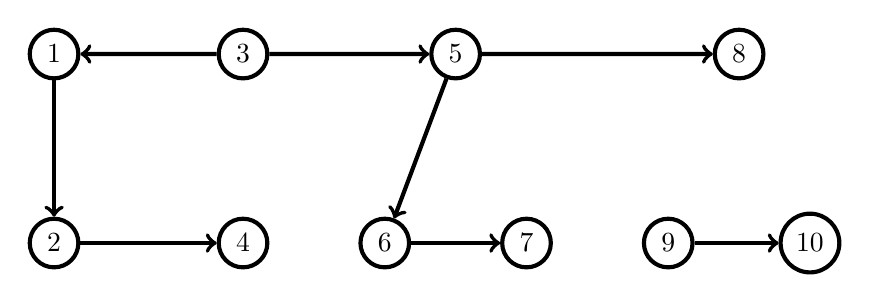
\begin{tikzpicture}[line width=1.5,scale=1.2]
 \node[circle,draw=black] (1) at (0,2) {$1$};
 \node[circle,draw=black] (2) at (0,0) {$2$};
 \node[circle,draw=black] (3) at (2,2) {$3$};
 \node[circle,draw=black] (4) at (2,0) {$4$};
 \node[circle,draw=black] (5) at (4.25,2) {$5$};
 \node[circle,draw=black] (6) at (3.5,0) {$6$};
 \node[circle,draw=black] (7) at (5,0) {$7$};
 \node[circle,draw=black] (8) at (7.25,2) {$8$};
 \node[circle,draw=black] (9) at (6.5,0) {$9$};
 \node[circle,draw=black] (10) at (8,0) {$10$};
		
 \draw[->] (1) edge (2);
 \draw[->] (2) edge (4);
 \draw[->] (3) edge (1) (3) edge (5);
 \draw[->] (5) edge (6) (5) edge (8); 
 \draw[->] (6) edge (7);
 \draw[->] (9) edge (10);
\end{tikzpicture}
\end{center} 
\end{bsp} 


\begin{thm} \label{thm:erreichbarkeit:ts} 
	Sei $D=(V,A)$ Digraph, der durch eine Adjazenzliste gegeben ist. Sei $s \in V$. Dann gilt für die Tiefensuche auf $D$ mit dem Startknoten $s$:
	\begin{enuma}
		\item Die Menge aller Knoten von $D$, die von $s$ aus durch einen Pfad erreichbar sind ist genau die Menge der Knoten, die während der Ausführung entdeckt werden. 
		\item $D$ enthält genau dann einen von $s$ aus erreichbaren Zyklus, wenn während der Ausführung beim Sondieren einer der Kanten $(u,v)$ die Farbe von $v$ grau ist. 
	\end{enuma} 
\end{thm}
\begin{proof}
	Wir bezeichnen die Tiefensuche kurz als TS.
		
	\condclearpage 
	
	(a): Seien $u_1,\ldots,u_k$ alle Knoten, die während der Ausführung entdeckt werden und seien $u_1,\ldots,u_k$ in dieser Reihenfolge entdeckt. Dann ist $u_1$ von $s$ aus erreichbar, denn $u_1=s$. Die TS für einen Knoten $u_j$ mit $j > 1$ wird aus einer TS für einen Knoten $u_i$ aufgerufen, der im Moment des Aufrufs von $TS(u_j)$ bereits entdeckt ist. Man hat also $j< i$. Wenn $u_j$ von $s$ aus erreichbar ist, so ist auch $u_i$ von $s$ aus erreichbar, da $(u_i,u_j)$ eine Kante von $G$ ist. Somit folgt durch Induktion über $j$, das jeder Knoten $u_j$ von $s$ aus erreichbar ist. 
	
	\condclearpage 
	
	Umgekehrt zeigen wir, dass jeder Knoten $v \in V$, der von $s$ aus erreichbar ist, während der Ausführung entdeckt wird. Sei $(v_0,\ldots,v_k)$ ein Pfad von $s$ nach $v$. Wir zeigen, dass jeder Knoten $v_j$ dieses Pfades entdeckt wird. Für $v_0=s$ gilt die Aussage offensichtlich. Wird ein Knoten $v_j$ mit $j < k$ entdeckt, so entdeckt man den Knoten $v_{j+1}$ spätestens beim Sondieren der Kante $(v_j,v_{j+1})$ innerhalb der TS für $v_j$. Es kann als durch Induktion über $j$ gezeigt werden, dass alle $v_j$ und insbesondere auch $v_k=v$ entdeckt werden.
	
	\condclearpage 
	
	(b): Der Beweis von (b) ist analog zum Beweis von (a) und wird hier nicht angeführt. (Aufgabe)
\end{proof}


\begin{bem}
Eine erste wichtige Eigenschaft der Tiefensuche ist der Zusammenhang von Entdeckungszeit und Abarbeitungszeit eines Knotens.
Es stellt sich heraus, dass diese Zeitpunkte im folgenden Sinne eine \emph{Klammerstruktur} aufweisen:
Stellen wir die Entdeckungszeit eines Knotens $u$ durch den Ausdruck \glqq $(u$\grqq\ und die Abarbeitungszeit von~$u$ durch den Ausdruck \glqq $u)$\grqq\ dar, dann ergibt die gesamte Historie, über alle Knoten des (Di)Graphen hinweg gesehen, einen korrekt geklammerten Ausdruck.
\end{bem} 

\begin{bsp} 
Zur Illustration dieses Zusammenhangs sehen wir uns wieder die Tiefensuche aus Beispiel~\ref{bsp:tiefensuche} an.
Die Daten der Zeitstempel sind in folgender Tabelle zusammengefasst:
\begin{table}[H]
\centering
\begin{tabular}{|c|c|c|c|c|c|c|c|c|c|c|}
\hline
\textbf{Knoten $u$}        & \textbf{1} & \textbf{2} & \textbf{3} & \textbf{4} & \textbf{5} & \textbf{6} & \textbf{7} & \textbf{8} & \textbf{9} & \textbf{10} \\ \hline
\textbf{$\cc{Grau}[u]$}    & 2          & 3          & 1          & 4          & 8          & 9          & 10         & 13         & 17         & 18          \\ \hline
\textbf{$\cc{Schwarz}[u]$} & 7          & 6          & 16         & 5          & 15         & 12         & 11         & 14         & 20         & 19          \\ \hline
\end{tabular}
\end{table}
Nach obiger Vorschrift können wir damit den zugehörigen Klammerausdruck
\[
(3\ (1\ (2\ (4\ 4)\ 2)\ 1)\ (5\ (6\ (7\ 7)\ 6)\ (8\ 8)\ 5)\ 3)\ (9\ (10\ 10)\ 9)
\]
ablesen.

Eine andere Möglichkeit diese Klammerstruktur auszudrücken ist im folgenden Satz festgehalten:
\end{bsp} 

\begin{defn}
	Bzgl. einer vollständigen Tiefensuche auf $D=(V,A)$ mit Startknoten $s$ definieren die \textbf{Lebenszeitintervall} eines Knoten $v \in V$ als die Menge
	\[
			I_u:=\setcond{t \in \Z}{ \cc{Grau}[u] \le t \le \cc{Schwarz}[u]}. 
	\]
\end{defn} 

\begin{thm}[Klammerungstheorem]
\label{thm:klammerung}
Bei der vollständigen Tiefensuche auf einem Digraphen $D=(V,A)$ ist für jedes Paar von Knoten $u$ und $v$ genau eine der drei folgenden Bedingungen erfüllt:
\begin{enuma}

 \item $I_u \cap I_v = \emptyset$  und weder $u$ noch $v$ ist im Tiefensuchwald ein Nachfahre des anderen.

 \item $I_u \subseteq I_v$ und $u$ ist im Tiefensuchwald ein Nachfahre von $v$.

 \item $I_v \subseteq I_u$ und $v$ ist im Tiefensuchwald ein Nachfahre von $u$.

\end{enuma}
\end{thm}
\begin{proof}
	Die Aussage ist symmetrisch bzgl. $u$ und $v$. Wir  nehmen also ohne Beschränkung der Allgemeinheit an, dass während der Ausführung der vollständigen Tiefensuche der Knoten $u$ als erster entdeckt wurde. Ist die Tiefensuche für $v$ nach der Terminierung der Tiefensuche für $u$ aufgerufen worden, so gilt $I_u \cap I_v = \emptyset$. Ansonsten ist die Tiefensuche für $v$ vor der Terminierung der Tiefensuche für $u$ aufgerufen worden. Das bedeutet, dass der Knoten $v$ während der Ausführung von $u$ entdeckt worden ist. Der Aufruf von $TS(v)$ erfolgt also durch eine Folge der geschachtelten rekursiven Aufrufen 
	\[
		TS(u) \xrightarrow{} \cdots \xrightarrow{} TS(v) 
	\] 
	Somit terminiert $TS(v)$ vor $TS(u)$. Es gilt also $I_v \subseteq I_u$ ist $v$ ist Nachfahre von $u$. 
\end{proof}

\begin{bem}
Als direkte Konsequenz des Klammerungstheorems erhalten wir eine Charakterisierung der Nachfahren im Tiefensuchwald eines gegebenen Knotens.
\end{bem} 

\begin{kor}
\label{cor:nachfahre-tiefenwald}
Der Knoten $v$ ist in einem Tiefensuchwald eines Digraphen genau dann ein echter Nachfahre eines Knotens $u$, wenn
\[
\cc{Grau}[u] < \cc{Grau}[v] < \cc{Schwarz}[v]  < \cc{Schwarz}[u].
\]
\end{kor}

\begin{bem} 
Eine alternative Charakterisierung der Nachfahreneigenschaft in Tiefensuchwäldern, die allerdings über die Farben der Knoten während der Suche geht, wird uns später bei den Anwendungen der Tiefensuche nützlich sein. 
\end{bem} 

\begin{thm}[Theorem der weißen Pfade]
\label{thm:weisse-pfade-thm}
Der Knoten $v$ ist in einem Tiefensuchwald eines Digraphen $D=(V,A)$ genau dann ein Nachfahre eines Knotens $u$, wenn es zum Zeitpunkt $\cc{Grau}[u]$, zu dem die Durchmusterung den Knoten~$u$ entdeckt hat, einen Pfad von $u$ nach $v$ gibt, der, bis auf den Knoten $u$, nur aus weißen Knoten besteht.
\end{thm}
\begin{proof} 
Komplett analog zum Beweis von Theorem~\ref{thm:erreichbarkeit:ts}(b). 
\end{proof} 



\begin{defn}
\label{def:kantenarten-tiefensuche}
Die Kanten $(u,v) \in A$ die bei einer Tiefensuche auf $D=(V,A)$ sondiert werden, werden in Abhängigkeit davon, welche Farbe $v$ beim Sondieren von $(u,v)$ hat und in welchem Zusammenhang $\cc{Grau}[u]$  und $\cc{Grau}[v]$ stehen, in die folgenden Arten unterteilt: 
\begin{center} 
\begin{tabular}{l|l}
	Art von $(u,v) \in A$ & Bedingung beim Sondieren 
	\\ \hline 
	\textbf{Baumkante} & $\cc{Farbe}[v]=\cc{weiss}$ 
\\	\textbf{Rückwärtskante} & $\cc{Farbe}[v] = \cc{grau}$
\\ \textbf{Vorwärtskante} & $\cc{Farbe}[v] = \cc{schwarz}$, $\cc{Grau}[u] < \cc{Grau}[v]$
\\ \textbf{Querkante} & $\cc{Farbe}[v] = \cc{schwarz}$, $\cc{Grau}[u] > \cc{Grau}[v]$
\end{tabular} 
\end{center} 
Baumkanten sind die Kanten des Tiefensuchwalds $D_\pi$. 
\end{defn}

\begin{bsp} Im Fall der Adjazensliste 
	\begin{align*}
		 1: & \ [2,4] 
		 \\ 2: & \  [3,4]
		 \\ 3: & \ [1]
		 \\  4: & \ [3]
	\end{align*}
 wird  während der Ausführung von $\cc{Tiefensuche}(1)$ die folgende Unterteilung der Kanten in die vier Arten festgelegt: 
	\begin{center} 
	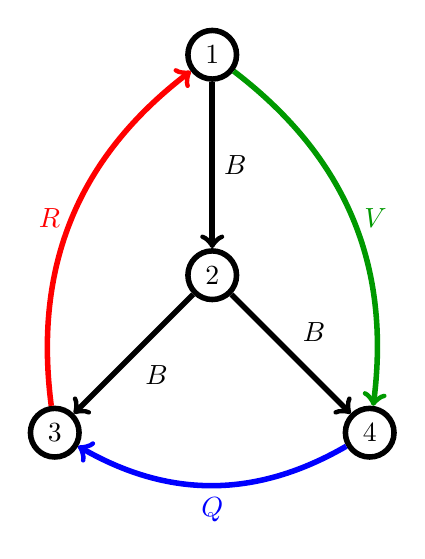
\begin{tikzpicture}[line width=2,scale=2]
		\node[circle,draw=black] (1) at (0,3.4) {$1$};
		\node[circle,draw=black] (2) at (0,2) {$2$};
		\node[circle,draw=black] (3) at (-1,1) {$3$};
		\node[circle,draw=black] (4) at (1,1) {$4$};
		\draw[->] (1) edge node[right]{$B$}(2) (2) edge node[below right]{$B$} (3) (2) edge node[above right]{$B$} (4);
		\draw[->,red] (3) edge[bend left] node[left]{$R$} (1);
		\draw[->,green!60!black]  (1) edge[bend left] node[right]{$V$} (4);
		\draw[->,blue] (4) edge[bend left] node[below]{$Q$} (3);
	\end{tikzpicture} 
	\end{center} 
\end{bsp} 

\begin{prop} 
	Wird die Unterteilung der Kanten in die vier Arten Baum-, Rückwärts- Vorwärts- und Querkante im Rahmen der vollständigen Tiefensuche durchgeführt, so ist jede Kante, welche zwei Bäume des Tiefensuchbaums verbindet eine Querkante. 
\end{prop} 


%\begin{remark}
%Durch die TS können die Kanten $(u,v)$ des Graphen in drei Arten klassifiziert werden: die Vorwärtskanten (beim sondieren von $(u,v)$ ist $v$ weiß), die Rückwärtskarten (beim sondieren der Kante ist $v$ grau) und die Querkanten (beim Sondieren der Kante ist $v$ schwarz). Die Menge aller  $\{u,v\}$ derart, dass $(u,v) \in E$ als ein Vorwärtskante klassifiziert wurde, ist Kantenmenge eines Baums. Die Knotenmenge dieses Baums ist die Menge aller entdeckten Knoten.
%\end{remark}

\begin{bsp} 
Wir schauen uns wiederum die Tiefensuche aus Beispiel~\ref{bsp:tiefensuche} an und, basierend auf den bereits erhobenen Daten, stellen wir die Klassifikation der Kanten des bearbeiteten Digraphen farbkodiert in folgender Abbildung dar.
Dabei sind Baumkanten schwarz, Rückwärtskanten rot, Vorwärtskanten blau und Querkanten grün markiert.

\begin{center} 
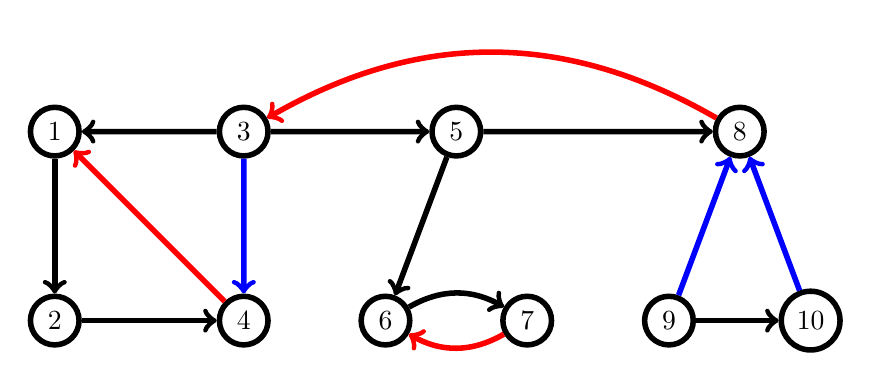
\begin{tikzpicture}[line width=2,scale=1.2]
 \node[circle,draw=black] (1) at (0,2) {$1$};
 \node[circle,draw=black] (2) at (0,0) {$2$};
 \node[circle,draw=black] (3) at (2,2) {$3$};
 \node[circle,draw=black] (4) at (2,0) {$4$};
 \node[circle,draw=black] (5) at (4.25,2) {$5$};
 \node[circle,draw=black] (6) at (3.5,0) {$6$};
 \node[circle,draw=black] (7) at (5,0) {$7$};
 \node[circle,draw=black] (8) at (7.25,2) {$8$};
 \node[circle,draw=black] (9) at (6.5,0) {$9$};
 \node[circle,draw=black] (10) at (8,0) {$10$};

% Baumkanten
 \draw[->] (1) edge (2);
 \draw[->] (2) edge (4);
 \draw[->] (3) edge (1) (3) edge (5);
 \draw[->] (5) edge (6) (5) edge (8); 
 \draw[->] (6) to[bend left] (7);
 \draw[->] (9) edge (10);

% Rückwärtskanten
 \draw[->,red] (4) edge (1);
 \draw[->,red] (7) to[bend left] (6);
 \draw[->,red] (8) to[bend right] (3);

% Vorwärtskanten
 \draw[->,blue] (3) edge (4);
 \draw[->,blue] (9) edge (8);
 \draw[->,blue] (10) edge (8); 
	
% Querkanten (keine vorhanden..)
	
\end{tikzpicture}
\end{center} 
\end{bsp} 


\begin{thm}
Bei einer Tiefensuche auf einem ungerichteten Graphen $G$ ist jede Kante entweder eine Baumkante oder eine Rückwärtskante.
\end{thm}

\begin{proof}
Sei $(u,v)$ eine beliebige Kante von~$G$ und seien die Knoten so bezeichnet, dass $\cc{Grau}[u] < \cc{Grau}[v]$ gilt.
Die Tiefensuche muss daher den Knoten~$v$ entdeckt und fertig abgearbeitet haben, bevor~$u$ fertig abgearbeitet ist.
In der Zwischenzeit ist der Knoten~$u$ stets grau.
Falls die Durchmusterung die Kante zuerst in der Richtung von~$u$ nach~$v$ sondiert, so ist~$v$ bis dahin unentdeckt (also weiß) gewesen, da die Kante sonst bereits in Gegenrichtung sondiert worden wäre.
Mit anderen Worten, die Kante $(u,v)$ ist eine Baumkante.

Falls nun die Durchmusterung die Kante zuerst in der Richtung von~$v$ nach~$u$ sondiert, so ist die Kante $(u,v)$ eine Rückwärtskante, da~$u$ zu dem Zeitpunkt der Sondierung noch grau ist.
\end{proof}


\begin{bem}
	Analog zur diskutierten Breitensuche kann man eine \emph{Tiefensuche} auch ohne Rekursion umsetzen.
	Dies hat praktische Vorteile, weil der Programmstack nicht  belastet wird.
	Dazu ersetzt man die Warteschlange $Q$ durch einen sogenannten \emph{Stack} ($=$ \emph{Stapel}). Für die Tiefensuche kann ein Stack auf der Basis von einem Array umgesetzt werden. 
	
	Hier eine ziemlich direkte Konvertierung der rekursiven Umsetzung. Wir gehen von einem zugrundeliegenden Stack $S$ aus. Als $\cc{Top}(S)$ bezeichnen wir das oberste Element des Stacks . Durch $\cc{Pop}(S)$ erfolgt die Entfernung und Rückgabe des obersten Elements. Durch $\cc{Push}(S,u)$ wird ein neues Element $u$ auf den Stack gelegt. Die Elemente $N[u]$ indexieren wir mit Zahlen $0$ bis $\deg(u)-1$, wobei hier $\deg(u)$ der Grad des Knotens $u$ ist. Wir führen ein Array $\cc{ind}$ ein, in dem durch $\cc{ind}[u]$ notiert wird, dass beim sondieren der Nachbarn von $u \in V$  der Knoten $v=N[u][\cc{ind}[u]]$ als  nächster dran ist. Ist $v= \deg(u)$, so hat man alle Nachbarn von $u$ sondiert. Wir setzen am Anfang $\cc{ind}[u]=0$ für alle $u \in V$, färben den Startknoten $s$ grau und legen $s$ auf $S$. Auf diese Weise lassen sich mit Hilfe von $S$ und $\cc{ind}$ die gerade laufenden rekursiven Aufrufe der Tiefensuche simulieren: 
	
	\begin{algorithm}[H]
		\caption{$\cc{Tiefensuche-mit-Stack}(s)$} 
		\begin{algorithmic}[1]
			\STATE Stack $S$ für höchstens $|V|$ Elemente anlegen
			\STATE $\cc{Farbe}[s] = \cc{grau}$ 
			\STATE $\cc{push}(S,s)$
			\STATE Liste $\cc{Ind}$  mit $\cc{Ind}[u]=0$ für alle $u \in V$ anlegen
			\WHILE{$S$ nicht leer }
			\STATE $u:= \cc{top}(S)$ \quad \COMMENT{Suche für $u$ läuft weiter}
			\IF{$\cc{ind}[u] = \deg(u)$} 
			\STATE $\cc{pop}(S)$   \quad \COMMENT{Suche für $u$ wird beendet}
			\STATE $\cc{Farbe}[u] := \cc{schwarz}$
			\ELSE
			\STATE $v=N[u][\cc{ind}[u]]$ \quad \COMMENT{Sondierung der Nachbarn von $u$ wird fortgesetzt} 
			\STATE $\cc{ind}[u]:=\cc{ind}[u]+1$				
			\IF{$\cc{Farbe}[v] = \cc{weiss}$}
			\STATE $\cc{Farbe}[v] = \cc{grau}$ \quad \COMMENT{Neuer Knoten ist entdeckt}
			\STATE $\cc{push}(S,v)$ \quad \COMMENT{Suche für $v$ wird gestartet}
			\ENDIF 
			\ENDIF 
			\ENDWHILE  
		\end{algorithmic}
	\end{algorithm}
	
	Die weiteren Daten, die man im Rahmen der rekursiven Tiefensuche berechnen kann, kann man auch in der obigen iterativen Version an den entsprechenden Stellen berechnen. 
\end{bem}




\subsection{Anwendung I -- Topologisches Sortieren}

\begin{defn} 
Sei $D=(V,A)$ ein Digraph mit $n$ Knoten.
Eine \emph{topologische Sortierung} von $D$ ist eine Anordnung $v_1,\ldots,v_n$ seiner Knoten, so dass $i < j$ gilt, falls $(v_i,v_j) \in A$ eine Kante in~$D$ ist.
Das heißt, der Startknoten einer jeden Kante kommt in der Anordnung vor dem Endknoten.
\end{defn} 

\begin{bem}
Man kann die topologische Sortierung auch als horizontale Anordnung der Knoten von~$D$ auffassen, so dass jede Kante von links nach rechts zeigt.

Diese Veranschaulichung zeigt, dass es nicht möglich ist, einen Digraphen topologisch zu sortieren, wenn er einen Zyklus enthält.
Im Folgenden werden wir sehen, wie man mit einer Tiefensuche jeden \emph{azyklischen} Digraphen topologisch sortieren kann.
Als Konsequenz ergibt sich:
\end{bem} 

\begin{prop}
Ein Digraph besitzt genau dann eine topologische Sortierung, wenn er azyklisch ist.
\end{prop}

\begin{bem}
	Eine Anwendung des topologischen Sortierens ist \textbf{makefile}. Die Kanten des Diagraphen sind durch  die Paare target-prerequisite gegeben. Die targets sollen in einer topologisch sortierten Reihenfolge abgearbeitet werden. 
\end{bem} 


\begin{bem} 
Das topologische Sortieren kann also als Methode verstanden werden, um zu testen ob es Zyklen im Eingabegraphen gibt.
Eine andere Anwendung ist das Sequenzieren von Aufträgen (engl.~\emph{scheduling}).
Zum Beispiel hilft die topologische Sortierung zu entscheiden, in welcher Reihenfolge einzelne Teilprojekte in einem großen Programmierprojekt kompiliert werden sollten.
\end{bem} 



\begin{thm}
	Nach der Ausführung der vollständigen Tiefensuche auf einem azyklischen Digraphen $D=(V,A)$ ist die Anordnung der Knoten $u \in V$ in der absteigenden Reihenfolge nach $\cc{Schwarz}[u]$ eine topologische Sortierung. Diese Anordnung kann während der Tiefensuche in der Zeit $\Theta(|V|+|A|)$ berechnet werden. 
\end{thm}

\begin{proof}
	Wir betrachten eine Kante $(u,v)$. Ist $v$ vor $u$ entdeckt worden, so wird während der Ausführung von $TS(u)$ der Knoten $u$ nicht entdeckt, denn sonst gäbe es einen $(v,u)$-Pfad und somit auch einen Zyklus in $D$. Das bedeutet, dass in diesem Fall $TS(v)$ vor $TS(u)$ terminiert. Es gilt also $\cc{Schwarz}[v] \le \cc{Schwarz}[u]$. 
	
	Wird $u$ vor $v$ entdeckt, so wird $v$ während der Ausführung von $TS(u)$ spätestens beim Sondieren von $(u,v)$ entdeckt. In diesem Fall terminiert $TS(v)$ ebenfalls vor $TS(u)$. Somit gilt auch in diesem Fall $\cc{Schwarz}[v] \le \cc{Schwarz}[u]$.
\end{proof}




\subsection{Anwendung II -- Starke Zusammenhangskomponenten}

\begin{defn}
Eine inklusionsmaximale Teilmenge $K \subseteq V$ der Knoten eines gegebenen Digraphen $D=(V,A)$ heißt \emph{starke Zusammenhangskomponente}, wenn es für jedes Paar von Knoten $u,v \in K$ sowohl einen $(u,v)$-Pfad als auch einen $(v,u)$-Pfad in~$D$ gibt.
Das heißt, die Knoten $u$ und $v$ sind vom jeweils anderen aus erreichbar.
\end{defn} 

\begin{bsp}
\label{bsp:starke-zusammenhangskomponenten}
Die starken Zusammenhangskomponenten des Digraphen aus Beispiel~\ref{bsp:tiefensuche} bestehen aus den Knoten gleicher Farbe in folgender Abbildung:

\hfill
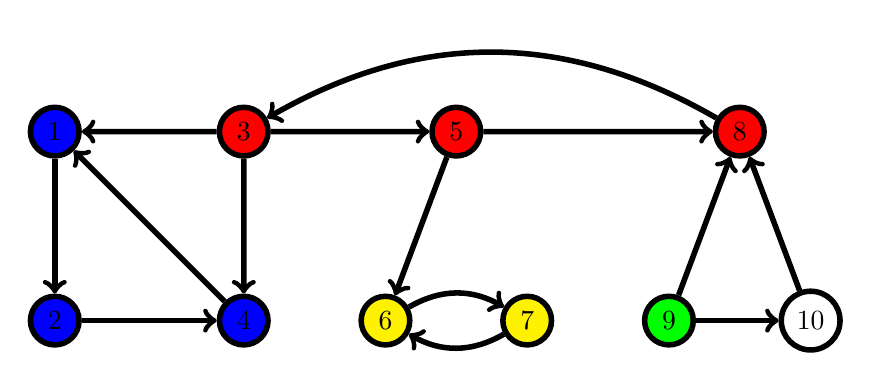
\begin{tikzpicture}[line width=2,scale=1.2]
 \node[fill=blue,circle,draw] (1) at (0,2) {$1$};
 \node[fill=blue,circle,draw] (2) at (0,0) {$2$};
 \node[fill=red,circle,draw] (3) at (2,2) {$3$};
 \node[fill=blue,circle,draw] (4) at (2,0) {$4$};
 \node[fill=red,circle,draw] (5) at (4.25,2) {$5$};
 \node[fill=yellow,circle,draw] (6) at (3.5,0) {$6$};
 \node[fill=yellow,circle,draw] (7) at (5,0) {$7$};
 \node[fill=red,circle,draw] (8) at (7.25,2) {$8$};
 \node[fill=green,circle,draw] (9) at (6.5,0) {$9$};
 \node[circle,draw=black] (10) at (8,0) {$10$};
		
 \draw[->] (1) edge (2);
 \draw[->] (2) edge (4);
 \draw[->] (3) edge (1) (3) edge (4) (3) edge (5);
 \draw[->] (4) edge (1);
 \draw[->] (5) edge (6) (5) edge (8); 
 \draw[->] (6) to[bend left] (7);
 \draw[->] (7) to[bend left] (6);
 \draw[->] (8) to[bend right] (3);
 \draw[->] (9) edge (8) (9) edge (10);
 \draw[->] (10) edge (8); 
\end{tikzpicture}
\hfill\,
\end{bsp}

\begin{bem}
Als weitere wichtige Anwendung der Tiefensuche zeigen wir hier, wie man mit ihrer Hilfe einen Digraphen in dessen starken Zusammenhangskomponenten zerlegen kann, das heißt, wir suchen eine Partition $V = K_1 \cup K_2 \cup \ldots \cup K_r$ der Knotenmenge von~$D$, so dass jede Teilmenge $K_i \subseteq V$ eine starke Zusammenhangskomponente ist.
Eine solche Zerlegung liegt vielen Algorithmen auf Digraphen zugrunde, da sie einen Ansatz mittels des Schemas Teile-und-Beherrsche erlaubt:
Nach der erfolgten Zerlegung des Digraphen arbeitet der jeweilige Algorithmus auf den einzelnen Komponenten separat und vereinigt dann die Lösungen entsprechend der Verbindungsstruktur der Komponenten untereinander.

Der Algorithmus, den wir hier untersuchen wollen, basiert darauf eine Tiefensuche auf dem gegebenen Digraphen $D=(V,A)$ und danach eine weitere auf seinem \emph{transponierten Graphen} $D^T = (V,A^T)$ zu machen, dessen Kantenmenge durch $A^T = \{(u,v) \in V \times V : (v,u) \in A\}$ definiert ist.
Wir erhalten also $D^T$ aus $D$ indem wir die Orientierung aller Kanten von $D$ umdrehen.

Ein Knoten $v$ ist in $D$ genau dann von einem anderen Knoten $u$ aus erreichbar, wenn~$u$ in $D^T$ von $v$ aus erreichbar ist.
Es gilt weiterhin die folgende wichtige Eigenschaft:
\end{bem} 

\begin{prop}
\label{beob:d-vs-dt}
Der zu einem Digraphen $D=(V,A)$ transponierte Graph $D^T$ hat dieselben starken Zusammenhangskomponenten wie~$D$.
\end{prop}

\begin{bem} 
Der konkrete Algorithmus zum Bestimmen der starken Zusammenhangskomponenten ist im folgenden Pseudocode angegeben.
Beachten Sie die Modifikation der Reihenfolge, in der die Knoten bei der zweiten Tiefensuche durchlaufen werden.

\begin{algorithm}[H]
\caption{$\cc{Starke-Zusammenhangskomponenten}(D)$}
 \begin{algorithmic}[1]
  \STATE\label{line:szhk0} $\cc{Vollständige-Tiefensuche}(D)$
  \STATE berechne $D^T$
  \STATE\label{line:szhk1} $\cc{Vollständige-Tiefensuche}(D^T)$ mit folgender Modifikation:
  \STATE\label{line:szhk2} $\qquad$ Durchlaufe die Hauptschleife (Zeilen~\ref{line:tiefensuche-hauptschleife-start}--\ref{line:tiefensuche-hauptschleife-ende}) der Tiefensuche auf $D^T$ in absteigender Reihenfolge des Arrays $\cc{Schwarz}$ von~$D$.
  \STATE gib die Knoten eines jeden Baumes im Tiefensuchwald $(D^T)_\pi$ als starke Zusammenhangskomponenten aus
 \end{algorithmic}
\end{algorithm}
\end{bem} 

\begin{thm}
\label{thm:starke-zshgk-laufzeit}
Ist ein Digraph $D=(V,A)$ als Adjazenzliste gegeben, so hat der Algorithmus $\cc{Starke-Zusammenhangskomponenten}(D)$ lineare Laufzeit, das heißt, er benötigt $\Theta(|V|+|A|)$ Zeiteinheiten.
\end{thm}

\begin{proof}
Die Tiefensuche in Zeile~\ref{line:szhk0} hat nach Theorem~\ref{thm:laufzeit-tiefensuche} lineare Laufzeit.
Die Berechnung des transponierten Graphen~$D^T$ kann auch in linearer Laufzeit geschehen, da~$D$ als Adjazenzliste gegeben ist (siehe Übungsblatt 7, Aufgabe (3)).
Die modifizizerte Tiefensuche auf~$D^T$ in den Zeilen~\ref{line:szhk1}-\ref{line:szhk2} läuft wieder in Zeit $\Theta(|V|+|A|)$.
Ebenso ist die Ausgabe der Bäume im Tiefensuchwald $(D^T)_\pi$ in linearer Laufzeit möglich.
\end{proof}

\begin{bem}
Die Idee hinter dem Algorithmus $\cc{Starke-Zusammenhangskomponenten}(D)$ beruht auf dem Konzept des \emph{Komponentengraphen} $D^K=(V^K,A^K)$ von $D=(V,A)$, der wie folgt definiert ist.
Seien $K_1,\ldots,K_r$ die starken Zusammenhangskomponenten von~$D$.
Dann setzen wir $V^K:=\{v_1,\ldots,v_r\}$, also je ein Knoten~$v_i$ für je eine starke Zusammenhangskomponente~$K_i$.
Es gibt eine Kante $(v_i,v_j) \in A^K$ genau dann, wenn es ein $u \in K_i$ und ein $w \in K_j$ gibt, so dass $(u,w) \in A$ eine Kante in~$D$ ist.
Der Komponentengraph~$D^K$ ensteht also aus~$D$ indem wir alle Kanten kontrahieren, deren Start- und Endknoten zur selben starken Zusammenhangskomponente gehören.
\end{bem}

\begin{bsp}
\label{bsp:komponentengraph}
Der Komponentengraph des Digraphen aus Beispiel~\ref{bsp:starke-zusammenhangskomponenten} in derselben Farbkodierung:

\hfill
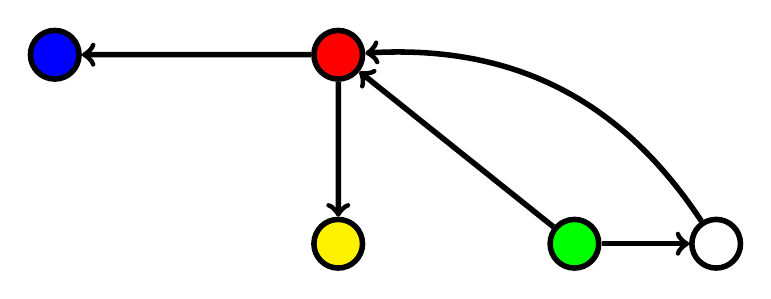
\begin{tikzpicture}[line width=2,scale=1.2]
 \node[fill=blue,circle,draw] (1) at (1,2) {$\phantom{1}$};
% \node[fill=blue,circle,draw] (2) at (0,0) {$2$};
% \node[fill=red,circle,draw] (3) at (2,2) {$3$};
% \node[fill=blue,circle,draw] (4) at (2,0) {$4$};
 \node[fill=red,circle,draw] (5) at (4,2) {$\phantom{5}$};
 \node[fill=yellow,circle,draw] (6) at (4,0) {$\phantom{6}$};
% \node[fill=yellow,circle,draw] (7) at (5,0) {$7$};
% \node[fill=red,circle,draw] (8) at (7.25,2) {$8$};
 \node[fill=green,circle,draw] (9) at (6.5,0) {$\phantom{9}$};
 \node[circle,draw=black] (10) at (8,0) {$\phantom{0}$};
		
 \draw[->] (5) edge (6) (5) edge (1); 
 \draw[->] (9) edge (5) (9) edge (10);
 \draw[->] (10) to[bend right] (5); 
\end{tikzpicture}
\hfill\,
\end{bsp}

\begin{bem}
Die wesentliche Eigenschaft des Komponentengraphen ist, dass er einen azyklischen Digraphen darstellt:
\end{bem} 

\begin{lem}
\label{lem:komponentengraph-azyklisch}
Sei $D=(V,A)$ ein Digraph und seien $K,K'$ zwei verschiedene starke Zusammenhangskomponenten von~$D$.
Seien weiterhin $u,v \in K$ und $u',v' \in K'$ Knoten der jeweiligen Komponente.
Falls $D$ einen $(u,u')$-Pfad enthält, so kann er nicht gleichzeitig auch einen $(v',v)$-Pfad enthalten.
\end{lem}

\begin{proof}
Angenommen, $D$ würde neben einem $(u,u')$-Pfad auch einen $(v',v)$-Pfad enthalten.
Da $K$ und $K'$ starke Zusammenhangskomponenten sind, könnten wir den $(u,u')$-Pfad zu einem $(u,v')$-Pfad und ebenso den $(v',v)$-Pfad zu einem $(v',u)$-Pfad erweitern.
Demnach wären die Knoten~$u$ und~$v'$ vom jeweils anderen aus erreichbar, was der Annahme widerspricht, dass $K$ und $K'$ verschieden sind.
\end{proof}

\begin{bem}
Für den Korrektheitsbeweis des angegebenen Algorithmus benötigen wir etwas mehr Verständnis der Beziehungen zwischen den während der Laufzeit erzeugten Zeitstempeln.
Wenn wir nachfolgend von Zeitpunkten der Entdeckung und Abarbeitung sprechen, dann beziehen wir uns stets auf die entsprechenden Zeitstempel der ersten Tiefensuche in Zeile~\ref{line:szhk0} von $\cc{Starke-Zusammenhangskomponenten}(D)$.

Für die Formulierung der Aussage erweitern wir zunächst die Begriffe der Entde\-ckungs- und Abarbeitungszeitpunkte von einzelnen Knoten auf Teilmengen von Knoten:
Für $U \subseteq V$ seien dazu
\[
\cc{Grau}(U) := \min_{u \in U} \cc{Grau}[u] \quad \text{ und } \quad\cc{Schwarz}(U) := \max_{u \in U} \cc{Schwarz}[u]
\]
der früheste Entdeckungszeitpunkt beziehungsweise der späteste Abarbeitungszeitpunkt eines Knotens aus~$U$.
\end{bem}

\begin{lem}
\label{lem:komponenten-zeitpunkte}
Sei $D=(V,A)$ ein Digraph und seien $K,K'$ zwei verschiedene starke Zusammenhangskomponenten von~$D$.
\begin{enumi}
 \item\label{lem:komponenten-zeitpunkte:primal} Falls eine Kante $(u,v) \in A$ mit $u \in K$ und $v \in K'$ existiert, so gilt
 \[
 \cc{Schwarz}(K) > \cc{Schwarz}(K').
 \]
 
 \item\label{lem:komponenten-zeitpunkte:transponiert} Falls eine Kante $(u,v) \in A^T$ mit $u \in K$ und $v \in K'$ existiert, so gilt
 \[
 \cc{Schwarz}(K) < \cc{Schwarz}(K').
 \]
\end{enumi}
\end{lem}

\begin{proof}
i): Wir unterscheiden Fälle danach welche der beiden starken Zusammenhangskomponenten zuerst entdeckt wird.

Sei zuerst angenommen, dass $\cc{Grau}(K) < \cc{Grau}(K')$ gilt und sei~$x$ der erste entdeckte Knoten in~$K$.
Zum Zeitpunkt $\cc{Grau}[x]$ sind alle anderen Knoten in~$K$ und alle Knoten in~$K'$ weiß.
In diesem Moment enthält~$D$ also Pfade von~$x$ zu jedem anderen Knoten in~$K$, die, bis auf~$x$ selbst, nur aus weißen Knoten bestehen.
Die Existenz der Kante $(u,v)$ von der Komponente~$K$ in die Komponente~$K'$ impliziert damit, dass ebenso Pfade von~$x$ zu jedem Knoten in~$K'$ bestehen, die, bis auf~$x$ selbst, nur aus weißen Knoten bestehen.
Nach dem Theorem~\ref{thm:weisse-pfade-thm} der weißen Pfade sind also alle Knoten in $K \cup K'$ Nachfahren von~$x$ im Tiefensuchwald und nach Korollar~\ref{cor:nachfahre-tiefenwald} erhalten wir $\cc{Schwarz}(K) = \cc{Schwarz}[x] > \cc{Schwarz}(K')$.

Sei nun angenommen, dass $\cc{Grau}(K) > \cc{Grau}(K')$ gilt und sei~$y$ der erste entdeckte Knoten in~$K'$.
Analog zu oben sind zum Zeitpunkt $\cc{Grau}[y]$ alle Knoten in~$K'$ mit einem Pfad von~$y$ aus erreichbar, der, bis auf~$y$ selbst, nur aus weißen Knoten besteht.
Wegen Theorem~\ref{thm:weisse-pfade-thm} sind damit alle Knoten aus~$K'$ Nachfahren von~$y$ im Tiefensuchwald und mit Korollar~\ref{cor:nachfahre-tiefenwald} gilt $\cc{Schwarz}[y] = \cc{Schwarz}(K')$.
Nach Annahme sind zum Zeitpunkt $\cc{Grau}[y]$ alle Knoten in~$K$ weiß.
Da die Kante $(u,v)$ von~$K$ nach~$K'$ existiert, folgt aus Lemma~\ref{lem:komponentengraph-azyklisch}, dass es keinen Pfad von einem Knoten in~$K'$ zu einem Knoten in~$K$ geben kann.
Da damit kein Knoten in~$K$ von~$y$ aus erreichbar ist, ist die ganze Komponente~$K$ zum Zeitpunkt $\cc{Schwarz}[y]$ noch immer weiß.
Als Konsequenz erhalten wir $\cc{Schwarz}[w] > \cc{Schwarz}[y]$, für jeden Knoten $w \in K$, und damit $\cc{Schwarz}(K) > \cc{Schwarz}(K')$.

ii): Nach Definition von $A^T$ ist $(v,u)$ Kante von~$D$.
Da nach Beobachtung~\ref{beob:d-vs-dt} die Teilmengen~$K$ und $K'$ starke Zusammenhangskomponenten von~$D^T$ sind, können wir Teil~i) anwenden und erhalten $\cc{Schwarz}(K) < \cc{Schwarz}(K')$.
\end{proof}

\begin{bem} 
In Worten ausgedrückt besagt das vorige Lemma, dass jede Kante von~$D$ (bzw.~$D^T$), die zwei verschiedene starke Zusammenhangskomponenten verbindet, von der Komponente mit dem späteren (bzw.~früheren) Abarbeitungszeitpunkt ausgeht.

Auf der Grundlage dieser Beobachtung können wir nun die Grundidee des Korrektheitsbeweises erläutern:
Die Tiefenssuche auf~$D^T$ startet in der starken Zusammenhangskomponente~$K_1$, die den zuletzt abgearbeiteten Knoten~$u_1$ der Tiefensuche auf~$D$ enthält.
Der transponierte Graph $D^T$ enthält nach Lemma~\ref{lem:komponenten-zeitpunkte}~\ref{lem:komponenten-zeitpunkte:transponiert} keine Kanten, die von~$K_1$ zu einer anderen starken Zusammenhangskomponente verlaufen.
Daher werden bei der Tiefensuche die von~$u_1$ aus startet genau die Knoten aus der Komponente~$K_1$ besucht.
Der Algorithmus wählt danach den Knoten~$u_2$ außerhalb der Komponente~$K_1$, der als letztes unter den verbleibenden Knoten bei der Tiefensuche auf~$D$ abgearbeitet wurde und besucht wie zuvor, alle Knoten der starken Zusammenhangskomponente~$K_2$, die~$u_2$ enthält.
Dies geht iterativ weiter bis alle Tiefensuchbäume erstellt sind, und wir sehen, dass diese den starken Zusammenhangskomponenten entsprechen.
\end{bem} 

\begin{thm}
$\cc{Starke-Zusammenhangskomponenten}(D)$ bestimmt die starken Zusammenhangskomponenten eines Digraphen~$D=(V,A)$ korrekt.
\end{thm}

\begin{proof}
Wir argumentieren über vollständige Induktion nach der Anzahl der Tiefensuchbäume, die bei der Tiefensuche auf $D^T$ in den Zeilen~\ref{line:szhk1}-\ref{line:szhk2} des Algorithmus $\cc{Starke-Zusammenhangskomponenten}(D)$ gefunden werden und zeigen, dass jeder solche Baum eine starke Zusammenhangskomponente bildet.
Die konkrete Aussage, die wir per Induktion beweisen, ist: \glqq Die ersten $k$ Tiefensuchbäume, die in den Zeilen~\ref{line:szhk1}-\ref{line:szhk2} erzeugt werden, sind starke Zusammenhangskomponenten von~$D$.\grqq

Der Induktionsanfang ist mit $k=0$ klar.
Für den Induktionsschritt, sei $B \subseteq V$ der $(k+1)$-te erzeugte Baum bei der Tiefensuche auf~$D^T$.
Sei weiterhin $u \in B$ die Wurzel dieses Baumes und $K \subseteq V$ die starke Zusammenhangskomponente, die~$u$ enthält.
Für jede starke Zusammenhangskomponente $K' \neq K$, die bereits besucht wurde, gilt $\cc{Schwarz}[u] = \cc{Schwarz}(K) > \cc{Schwarz}(K')$, wegen der Reihenfolge in der die Knoten in Zeile~\ref{line:szhk2} durchlaufen werden.
Wegen der Induktionsannahme sind zum Zeitpunkt zu dem die Suche den Knoten~$u$ besucht, alle anderen Knoten von~$K$ weiß.
Nach dem Theorem~\ref{thm:weisse-pfade-thm} der weißen Pfade sind daher alle anderen Knoten in~$K$ Nachfahren von~$u$ in dessen Tiefensuchbaum.

Weiterhin müssen nach Induktionsannahme und Lemma~\ref{lem:komponenten-zeitpunkte}~\ref{lem:komponenten-zeitpunkte:transponiert} alle Kanten von~$D^T$, die aus $K$ herausführen, zu starken Zusammenhangskomponenten verlaufen, die bereits entdeckt wurden.
Damit wird kein Knoten außerhalb von~$K$ ein Nachfahre von~$u$ bei der Tiefensuche auf~$D^T$.
Das heißt, dass die Knoten des Tiefensuchbaumes von~$D^T$, der von~$u$ ausgeht, eine starke Zusammenhangskomponente bilden, und der Induktionsschritt ist gezeigt.
\end{proof}


\begin{bem}
	Die Präsentation der Tiefensuche basiert auf  \cite{CLRS17}.
\end{bem}   

\appendix 






%\begin{thebibliography}{AAA}
%	\bibitem[Rud]{Rud} Walter Rudin: Analysis. 4. Auflage, Oldenbourg 2009, 408~Seiten.  (Eines der Standardlehrbücher zur Analysis. Englisches Original ``Principles of Mathematical Analysis)
%	\bibitem[Dem]{Dem} Boris Pavlovich Demidovitch: A Collection of Problems and Exercises in Mathematical Analysis, 11. Auflage, 1995, in Russisch (Über 4000 Aufgaben zu verschiedenen Themen aus der Analysis)
%\end{thebibliography} 
%\bibliographystyle{amsalpha}
%\bibliography{lit}
% bibliography, glossary and index would go here.

\end{document}